%**************************************%
%*    Generated from PreTeXt source   *%
%*    on 2018-04-25T15:48:20+01:00    *%
%*                                    *%
%*   http://mathbook.pugetsound.edu   *%
%*                                    *%
%**************************************%
\documentclass[10pt,]{book}
%% Custom Preamble Entries, early (use latex.preamble.early)
%% Default LaTeX packages
%%   1.  always employed (or nearly so) for some purpose, or
%%   2.  a stylewriter may assume their presence
\usepackage{geometry}
%% Some aspects of the preamble are conditional,
%% the LaTeX engine is one such determinant
\usepackage{ifthen}
\usepackage{ifxetex,ifluatex}
%% Raster graphics inclusion
\usepackage{graphicx}
%% Colored boxes, and much more, though mostly styling
%% skins library provides "enhanced" skin, employing tikzpicture
%% boxes may be configured as "breakable" or "unbreakable"
\usepackage{tcolorbox}
\tcbuselibrary{skins}
\tcbuselibrary{breakable}
%% Hyperref should be here, but likes to be loaded late
%%
%% Inline math delimiters, \(, \), need to be robust
%% 2016-01-31:  latexrelease.sty  supersedes  fixltx2e.sty
%% If  latexrelease.sty  exists, bugfix is in kernel
%% If not, bugfix is in  fixltx2e.sty
%% See:  https://tug.org/TUGboat/tb36-3/tb114ltnews22.pdf
%% and read "Fewer fragile commands" in distribution's  latexchanges.pdf
\IfFileExists{latexrelease.sty}{}{\usepackage{fixltx2e}}
%% Text height identically 9 inches, text width varies on point size
%% See Bringhurst 2.1.1 on measure for recommendations
%% 75 characters per line (count spaces, punctuation) is target
%% which is the upper limit of Bringhurst's recommendations
\geometry{letterpaper,total={340pt,9.0in}}
%% Custom Page Layout Adjustments (use latex.geometry)
%% This LaTeX file may be compiled with pdflatex, xelatex, or lualatex
%% The following provides engine-specific capabilities
%% Generally, xelatex and lualatex will do better languages other than US English
%% You can pick from the conditional if you will only ever use one engine
\ifthenelse{\boolean{xetex} \or \boolean{luatex}}{%
%% begin: xelatex and lualatex-specific configuration
%% fontspec package will make Latin Modern (lmodern) the default font
\ifxetex\usepackage{xltxtra}\fi
\usepackage{fontspec}
%% realscripts is the only part of xltxtra relevant to lualatex 
\ifluatex\usepackage{realscripts}\fi
%% 
%% Extensive support for other languages
\usepackage{polyglossia}
%% Main document language is US English
\setdefaultlanguage{english}
%% Spanish
\setotherlanguage{spanish}
%% Vietnamese
\setotherlanguage{vietnamese}
%% end: xelatex and lualatex-specific configuration
}{%
%% begin: pdflatex-specific configuration
%% translate common Unicode to their LaTeX equivalents
%% Also, fontenc with T1 makes CM-Super the default font
%% (\input{ix-utf8enc.dfu} from the "inputenx" package is possible addition (broken?)
\usepackage[T1]{fontenc}
\usepackage[utf8]{inputenc}
%% end: pdflatex-specific configuration
}
%% Monospace font: Inconsolata (zi4)
%% Sponsored by TUG: http://levien.com/type/myfonts/inconsolata.html
%% See package documentation for excellent instructions
%% One caveat, seem to need full file name to locate OTF files
%% Loads the "upquote" package as needed, so we don't have to
%% Upright quotes might come from the  textcomp  package, which we also use
%% We employ the shapely \ell to match Google Font version
%% pdflatex: "varqu" option produces best upright quotes
%% xelatex,lualatex: add StylisticSet 1 for shapely \ell
%% xelatex,lualatex: add StylisticSet 2 for plain zero
%% xelatex,lualatex: we add StylisticSet 3 for upright quotes
%% 
\ifthenelse{\boolean{xetex} \or \boolean{luatex}}{%
%% begin: xelatex and lualatex-specific monospace font
\usepackage{zi4}
\setmonofont[BoldFont=Inconsolatazi4-Bold.otf,StylisticSet={1,3}]{Inconsolatazi4-Regular.otf}
%% end: xelatex and lualatex-specific monospace font
}{%
%% begin: pdflatex-specific monospace font
%% "varqu" option provides textcomp \textquotedbl glyph
%% "varl"  option provides shapely "ell"
\usepackage[varqu,varl]{zi4}
%% end: pdflatex-specific monospace font
}
%% Symbols, align environment, bracket-matrix
\usepackage{amsmath}
\usepackage{amssymb}
%% allow page breaks within display mathematics anywhere
%% level 4 is maximally permissive
%% this is exactly the opposite of AMSmath package philosophy
%% there are per-display, and per-equation options to control this
%% split, aligned, gathered, and alignedat are not affected
\allowdisplaybreaks[4]
%% allow more columns to a matrix
%% can make this even bigger by overriding with  latex.preamble.late  processing option
\setcounter{MaxMatrixCols}{30}
%%
%% Color support, xcolor package
%% Always loaded, for: add/delete text, author tools
\PassOptionsToPackage{usenames,dvipsnames,svgnames,table}{xcolor}
\usepackage{xcolor}
%%
%% Semantic Macros
%% To preserve meaning in a LaTeX file
%% Only defined here if required in this document
%% Used for warnings, typically bold and italic
\newcommand{\alert}[1]{\textbf{\textit{#1}}}
%% Used for inline definitions of terms
\newcommand{\terminology}[1]{\textbf{#1}}
%% Subdivision Numbering, Chapters, Sections, Subsections, etc
%% Subdivision numbers may be turned off at some level ("depth")
%% A section *always* has depth 1, contrary to us counting from the document root
%% The latex default is 3.  If a larger number is present here, then
%% removing this command may make some cross-references ambiguous
%% The precursor variable $numbering-maxlevel is checked for consistency in the common XSL file
\setcounter{secnumdepth}{3}
%% Environments with amsthm package
%% Theorem-like environments in "plain" style, with or without proof
\usepackage{amsthm}
\theoremstyle{plain}
%% Numbering for Theorems, Conjectures, Examples, Figures, etc
%% Controlled by  numbering.theorems.level  processing parameter
%% Always need a theorem environment to set base numbering scheme
%% even if document has no theorems (but has other environments)
\newtheorem{theorem}{Theorem}[section]
%% Only variants actually used in document appear here
%% Style is like a theorem, and for statements without proofs
%% Numbering: all theorem-like numbered consecutively
%% i.e. Corollary 4.3 follows Theorem 4.2
\newtheorem{lemma}[theorem]{Lemma}
\newtheorem{algorithm}[theorem]{Algorithm}
\newtheorem{proposition}[theorem]{Proposition}
%% Definition-like environments, normal text
%% Numbering is in sync with theorems, etc
\theoremstyle{definition}
\newtheorem{definition}[theorem]{Definition}
%% Remark-like environments, normal text
%% Numbering is in sync with theorems, etc
\theoremstyle{definition}
\newtheorem{remark}[theorem]{Remark}
%% Example-like environments, normal text
%% Numbering is in sync with theorems, etc
\theoremstyle{definition}
\newtheorem{example}[theorem]{Example}
\newtheorem{problem}[theorem]{Problem}
%% Numbering for inline exercises is in sync with theorems, normal text
\theoremstyle{definition}
\newtheorem{exercise}[theorem]{Exercise}
%% Localize LaTeX supplied names (possibly none)
\renewcommand*{\proofname}{Proof}
\renewcommand*{\chaptername}{Chapter}
%% Equation Numbering
%% Controlled by  numbering.equations.level  processing parameter
\numberwithin{equation}{section}
%% For improved tables
\usepackage{array}
%% Some extra height on each row is desirable, especially with horizontal rules
%% Increment determined experimentally
\setlength{\extrarowheight}{0.2ex}
%% Define variable thickness horizontal rules, full and partial
%% Thicknesses are 0.03, 0.05, 0.08 in the  booktabs  package
\makeatletter
\newcommand{\hrulethin}  {\noalign{\hrule height 0.04em}}
\newcommand{\hrulemedium}{\noalign{\hrule height 0.07em}}
\newcommand{\hrulethick} {\noalign{\hrule height 0.11em}}
%% We preserve a copy of the \setlength package before other
%% packages (extpfeil) get a chance to load packages that redefine it
\let\oldsetlength\setlength
\newlength{\Oldarrayrulewidth}
\newcommand{\crulethin}[1]%
{\noalign{\global\oldsetlength{\Oldarrayrulewidth}{\arrayrulewidth}}%
\noalign{\global\oldsetlength{\arrayrulewidth}{0.04em}}\cline{#1}%
\noalign{\global\oldsetlength{\arrayrulewidth}{\Oldarrayrulewidth}}}%
\newcommand{\crulemedium}[1]%
{\noalign{\global\oldsetlength{\Oldarrayrulewidth}{\arrayrulewidth}}%
\noalign{\global\oldsetlength{\arrayrulewidth}{0.07em}}\cline{#1}%
\noalign{\global\oldsetlength{\arrayrulewidth}{\Oldarrayrulewidth}}}
\newcommand{\crulethick}[1]%
{\noalign{\global\oldsetlength{\Oldarrayrulewidth}{\arrayrulewidth}}%
\noalign{\global\oldsetlength{\arrayrulewidth}{0.11em}}\cline{#1}%
\noalign{\global\oldsetlength{\arrayrulewidth}{\Oldarrayrulewidth}}}
%% Single letter column specifiers defined via array package
\newcolumntype{A}{!{\vrule width 0.04em}}
\newcolumntype{B}{!{\vrule width 0.07em}}
\newcolumntype{C}{!{\vrule width 0.11em}}
\makeatother
%% Figures, Tables, Listings, Named Lists, Floats
%% The [H]ere option of the float package fixes floats in-place,
%% in deference to web usage, where floats are totally irrelevant
%% You can remove some of this setup, to restore standard LaTeX behavior
%% HOWEVER, numbering of figures/tables AND theorems/examples/remarks, etc
%% may de-synchronize with the numbering in the HTML version
%% You can remove the "placement={H}" option to allow flotation and
%% preserve numbering, BUT the numbering may then appear "out-of-order"
%% Floating environments: http://tex.stackexchange.com/questions/95631/
\usepackage{float}
\usepackage{newfloat}
\usepackage{caption}%% Adjust stock figure environment so that it no longer floats
\SetupFloatingEnvironment{figure}{fileext=lof,placement={H},within=section,name=Figure}
\captionsetup[figure]{labelfont=bf}
%% http://tex.stackexchange.com/questions/16195
\makeatletter
\let\c@figure\c@theorem
\makeatother
%% Adjust stock table environment so that it no longer floats
\SetupFloatingEnvironment{table}{fileext=lot,placement={H},within=section,name=Table}
\captionsetup[table]{labelfont=bf}
%% http://tex.stackexchange.com/questions/16195
\makeatletter
\let\c@table\c@theorem
\makeatother
%% Footnote Numbering
%% We reset the footnote counter, as given by numbering.footnotes.level
\makeatletter\@addtoreset{footnote}{section}\makeatother
%% Program listing support: for listings, programs, and Sage code
\usepackage{listings}
%% We define the listings font style to be the default "ttfamily"
%% To fix hyphens/dashes rendered in PDF as fancy minus signs by listing
%% http://tex.stackexchange.com/questions/33185/listings-package-changes-hyphens-to-minus-signs
\makeatletter
\lst@CCPutMacro\lst@ProcessOther {"2D}{\lst@ttfamily{-{}}{-{}}}
\@empty\z@\@empty
\makeatother
\ifthenelse{\boolean{xetex}}{}{%
%% begin: pdflatex-specific listings configuration
%% translate U+0080 - U+00F0 to their textmode LaTeX equivalents
%% Data originally from https://www.w3.org/Math/characters/unicode.xml, 2016-07-23
%% Lines marked in XSL with "$" were converted from mathmode to textmode
\lstset{extendedchars=true}
\lstset{literate={ }{{~}}{1}{¡}{{\textexclamdown }}{1}{¢}{{\textcent }}{1}{£}{{\textsterling }}{1}{¤}{{\textcurrency }}{1}{¥}{{\textyen }}{1}{¦}{{\textbrokenbar }}{1}{§}{{\textsection }}{1}{¨}{{\textasciidieresis }}{1}{©}{{\textcopyright }}{1}{ª}{{\textordfeminine }}{1}{«}{{\guillemotleft }}{1}{¬}{{\textlnot }}{1}{­}{{\-}}{1}{®}{{\textregistered }}{1}{¯}{{\textasciimacron }}{1}{°}{{\textdegree }}{1}{±}{{\textpm }}{1}{²}{{\texttwosuperior }}{1}{³}{{\textthreesuperior }}{1}{´}{{\textasciiacute }}{1}{µ}{{\textmu }}{1}{¶}{{\textparagraph }}{1}{·}{{\textperiodcentered }}{1}{¸}{{\c{}}}{1}{¹}{{\textonesuperior }}{1}{º}{{\textordmasculine }}{1}{»}{{\guillemotright }}{1}{¼}{{\textonequarter }}{1}{½}{{\textonehalf }}{1}{¾}{{\textthreequarters }}{1}{¿}{{\textquestiondown }}{1}{À}{{\`{A}}}{1}{Á}{{\'{A}}}{1}{Â}{{\^{A}}}{1}{Ã}{{\~{A}}}{1}{Ä}{{\"{A}}}{1}{Å}{{\AA }}{1}{Æ}{{\AE }}{1}{Ç}{{\c{C}}}{1}{È}{{\`{E}}}{1}{É}{{\'{E}}}{1}{Ê}{{\^{E}}}{1}{Ë}{{\"{E}}}{1}{Ì}{{\`{I}}}{1}{Í}{{\'{I}}}{1}{Î}{{\^{I}}}{1}{Ï}{{\"{I}}}{1}{Ð}{{\DH }}{1}{Ñ}{{\~{N}}}{1}{Ò}{{\`{O}}}{1}{Ó}{{\'{O}}}{1}{Ô}{{\^{O}}}{1}{Õ}{{\~{O}}}{1}{Ö}{{\"{O}}}{1}{×}{{\texttimes }}{1}{Ø}{{\O }}{1}{Ù}{{\`{U}}}{1}{Ú}{{\'{U}}}{1}{Û}{{\^{U}}}{1}{Ü}{{\"{U}}}{1}{Ý}{{\'{Y}}}{1}{Þ}{{\TH }}{1}{ß}{{\ss }}{1}{à}{{\`{a}}}{1}{á}{{\'{a}}}{1}{â}{{\^{a}}}{1}{ã}{{\~{a}}}{1}{ä}{{\"{a}}}{1}{å}{{\aa }}{1}{æ}{{\ae }}{1}{ç}{{\c{c}}}{1}{è}{{\`{e}}}{1}{é}{{\'{e}}}{1}{ê}{{\^{e}}}{1}{ë}{{\"{e}}}{1}{ì}{{\`{\i}}}{1}{í}{{\'{\i}}}{1}{î}{{\^{\i}}}{1}{ï}{{\"{\i}}}{1}{ð}{{\dh }}{1}{ñ}{{\~{n}}}{1}{ò}{{\`{o}}}{1}{ó}{{\'{o}}}{1}{ô}{{\^{o}}}{1}{õ}{{\~{o}}}{1}{ö}{{\"{o}}}{1}{÷}{{\textdiv }}{1}{ø}{{\o }}{1}{ù}{{\`{u}}}{1}{ú}{{\'{u}}}{1}{û}{{\^{u}}}{1}{ü}{{\"{u}}}{1}{ý}{{\'{y}}}{1}{þ}{{\th }}{1}{ÿ}{{\"{y}}}{1}}
%% end: pdflatex-specific listings configuration
}
%% End of generic listing adjustments
%% Sage's blue is 50%, we go way lighter (blue!05 would work)
\definecolor{sageblue}{rgb}{0.95,0.95,1}
%% Sage input, listings package: Python syntax, boxed, colored, line breaking
%% To be flush with surrounding text's margins, set
%% xmargins to be sum of framerule, framesep, and epsilon (~0.25pt)
%% space between input/output comes from input style "belowskip",
%% by giving output an aboveskip of zero
\lstdefinestyle{sageinputstyle}{language=Python,breaklines=true,breakatwhitespace=true,%
basicstyle=\small\ttfamily,columns=fixed,frame=single,backgroundcolor=\color{sageblue},%
framerule=0.5pt,framesep=4pt,xleftmargin=4.75pt,xrightmargin=4.75pt}
%% Sage output, similar, but not boxed, not colored
\lstdefinestyle{sageoutputstyle}{language=Python,breaklines=true,%
breakatwhitespace=true,basicstyle=\small\ttfamily,columns=fixed,aboveskip=0pt}
%% The environments manufactured by the listings package
\lstnewenvironment{sageinput}
  {\lstset{style=sageinputstyle}}
  {}
\lstnewenvironment{sageoutput}
  {\lstset{style=sageoutputstyle}}
  {}
%% Fancy Verbatim for consoles, preformatted, code display
\usepackage{fancyvrb}
%% Pre-formatted text, a peer of paragraphs
\DefineVerbatimEnvironment{preformatted}{Verbatim}{}
%% Pre-formatted text, as panel of a sidebyside
%% Default alignment is the bottom of the box on the baseline
\DefineVerbatimEnvironment{preformattedbox}{BVerbatim}{}
%% More flexible list management, esp. for references and exercises
%% But also for specifying labels (i.e. custom order) on nested lists
\usepackage{enumitem}
%% Lists of exercises in their own section, maximum depth 4
\newlist{exerciselist}{description}{4}
\setlist[exerciselist]{leftmargin=0pt,itemsep=1.0ex,topsep=1.0ex,partopsep=0pt,parsep=0pt}
%% hyperref driver does not need to be specified, it will be detected
\usepackage{hyperref}
%% configure hyperref's  \url  to match listings' inline verbatim
\renewcommand\UrlFont{\small\ttfamily}
%% Hyperlinking active in PDFs, all links solid and blue
\hypersetup{colorlinks=true,linkcolor=blue,citecolor=blue,filecolor=blue,urlcolor=blue}
\hypersetup{pdftitle={MAS341: Graph Theory}}
%% If you manually remove hyperref, leave in this next command
\providecommand\phantomsection{}
%% Graphics Preamble Entries
    \usepackage{overpic,pict2e}
\usepackage{tikz}
\usetikzlibrary{arrows.meta}
%% If tikz has been loaded, replace ampersand with \amp macro
\ifdefined\tikzset
    \tikzset{ampersand replacement = \amp}
\fi
%% NB: calc redefines \setlength
\usepackage{calc}
%% used repeatedly for vertical dimensions of sidebyside panels
\newlength{\panelmax}
%% extpfeil package for certain extensible arrows,
%% as also provided by MathJax extension of the same name
%% NB: this package loads mtools, which loads calc, which redefines
%%     \setlength, so it can be removed if it seems to be in the 
%%     way and your math does not use:
%%     
%%     \xtwoheadrightarrow, \xtwoheadleftarrow, \xmapsto, \xlongequal, \xtofrom
%%     
%%     we have had to be extra careful with variable thickness
%%     lines in tables, and so also load this package late
\usepackage{extpfeil}
%% Custom Preamble Entries, late (use latex.preamble.late)
%% Begin: Author-provided packages
%% (From  docinfo/latex-preamble/package  elements)
%% End: Author-provided packages
%% Begin: Author-provided macros
%% (From  docinfo/macros  element)
%% Plus three from MBX for XML characters
\newcommand{\set}[1]{\{1,2,\dotsc,#1\,\}}
    \newcommand{\ints}{\mathbb{Z}}
    \newcommand{\posints}{\mathbb{N}}
    \newcommand{\rats}{\mathbb{Q}}
    \newcommand{\reals}{\mathbb{R}}
    \newcommand{\complexes}{\mathbb{C}}
    \newcommand{\twospace}{\mathbb{R}^2}
    \newcommand{\threepace}{\mathbb{R}^3}
    \newcommand{\dspace}{\mathbb{R}^d}
    \newcommand{\nni}{\mathbb{N}_0}
    \newcommand{\nonnegints}{\mathbb{N}_0}
    \newcommand{\dom}{\operatorname{dom}}
    \newcommand{\ran}{\operatorname{ran}}
    \newcommand{\prob}{\operatorname{prob}}
    \newcommand{\Prob}{\operatorname{Prob}}
    \newcommand{\height}{\operatorname{height}}
    \newcommand{\width}{\operatorname{width}}
    \newcommand{\length}{\operatorname{length}}
    \newcommand{\crit}{\operatorname{crit}}
    \newcommand{\inc}{\operatorname{inc}}
    \newcommand{\HP}{\mathbf{H_P}}
    \newcommand{\HCP}{\mathbf{H^c_P}}
    \newcommand{\GP}{\mathbf{G_P}}
    \newcommand{\GQ}{\mathbf{G_Q}}
    \newcommand{\AG}{\mathbf{A_G}}
    \newcommand{\GCP}{\mathbf{G^c_P}}
    \newcommand{\PXP}{\mathbf{P}=(X,P)}
    \newcommand{\QYQ}{\mathbf{Q}=(Y,Q)}
    \newcommand{\GVE}{\mathbf{G}=(V,E)}
    \newcommand{\HWF}{\mathbf{H}=(W,F)}
    \newcommand{\bfC}{\mathbf{C}}
    \newcommand{\bfG}{\mathbf{G}}
    \newcommand{\bfH}{\mathbf{H}}
    \newcommand{\bfF}{\mathbf{F}}
    \newcommand{\bfI}{\mathbf{I}}
    \newcommand{\bfK}{\mathbf{K}}
    \newcommand{\bfP}{\mathbf{P}}
    \newcommand{\bfQ}{\mathbf{Q}}
    \newcommand{\bfR}{\mathbf{R}}
    \newcommand{\bfS}{\mathbf{S}}
    \newcommand{\bfT}{\mathbf{T}}
    \newcommand{\bfNP}{\mathbf{NP}}
    \newcommand{\bftwo}{\mathbf{2}}
    \newcommand{\cgA}{\mathcal{A}}
    \newcommand{\cgB}{\mathcal{B}}
    \newcommand{\cgC}{\mathcal{C}}
    \newcommand{\cgD}{\mathcal{D}}
    \newcommand{\cgE}{\mathcal{E}}
    \newcommand{\cgF}{\mathcal{F}}
    \newcommand{\cgG}{\mathcal{G}}
    \newcommand{\cgM}{\mathcal{M}}
    \newcommand{\cgN}{\mathcal{N}}
    \newcommand{\cgP}{\mathcal{P}}
    \newcommand{\cgR}{\mathcal{R}}
    \newcommand{\cgS}{\mathcal{S}}
    \newcommand{\bfn}{\mathbf{n}}
    \newcommand{\bfm}{\mathbf{m}}
    \newcommand{\bfk}{\mathbf{k}}
    \newcommand{\bfs}{\mathbf{s}}
    \newcommand{\bijection}{\xrightarrow[\text{onto}]{\text{$1$--$1$}}}
    \newcommand{\injection}{\xrightarrow[]{\text{$1$--$1$}}}
    \newcommand{\surjection}{\xrightarrow[\text{onto}]{}}
    \newcommand{\nin}{\not\in}
    \newcommand{\prufer}{\mbox{prüfer}}
    \DeclareMathOperator{\fix}{fix}
    \DeclareMathOperator{\stab}{stab}
    \DeclareMathOperator{\var}{var}
    \newcommand{\inv}{^{-1}}
\newcommand{\lt}{<}
\newcommand{\gt}{>}
\newcommand{\amp}{&}
%% End: Author-provided macros
%% Title page information for book
\title{MAS341: Graph Theory}
\author{}
\date{}
\begin{document}
\frontmatter
%% begin: table of contents
%% Adjust Table of Contents
\setcounter{tocdepth}{1}
\renewcommand*\contentsname{Contents}
\tableofcontents
%% end:   table of contents
\mainmatter
\typeout{************************************************}
\typeout{Chapter 1 Introduction}
\typeout{************************************************}
\chapter[{Introduction}]{Introduction}\label{ch_intro}
\hypertarget{p-1}{}%
The first chapter is an introduction, including the formal definition of a graph and many terms we will use throughout, but more importantly, examples of these concepts and how you should think abotu them.%
\typeout{************************************************}
\typeout{Section 1.1 A first look a graphs}
\typeout{************************************************}
\section[{A first look a graphs}]{A first look a graphs}\label{s_intro_firstlook}
\typeout{************************************************}
\typeout{Subsection 1.1.1 The idea of a graph}
\typeout{************************************************}
\subsection[{The idea of a graph}]{The idea of a graph}\label{subsection-1}
\hypertarget{p-2}{}%
First and foremost, you should think of a graph as a certain type of picture, containing dots and lines connecting those dots, like so:%
\par
\hypertarget{p-3}{}%
We will typically use the letters \(G, H\), or \(\Gamma\) (capital Gamma) to denote a graph.  The ``dots'' or the graph are called \emph{vertices} or \emph{nodes}, and the lines between the dots are called \emph{edges}. Graphs occur frequently in the ``real world'', and typically how to show how something is connected, with the vertices representing the things and the edges showing connections.  \leavevmode%
\begin{itemize}[label=\textbullet]
\item{}\emph{Transit networks:} The London tube map is a graph, with the vertices representing the stations, and an edge between two stations if the tube goes directly between them.  More generally, rail maps in general are graphs, with vertices stations and edges representing line, and road maps as well, with vertices being cities, and edges being roads.%
\item{}\emph{Social networks:} The typical example would be Facebook, with the vertices being people, and edge between two people if they are friends on Facebook.%
\item{}\emph{Molecules in Chemistry:} In organic chemistry, molecules are made up of different atoms, and are often represented as a graph, with the atoms being vertices, and edges representing covalent bonds between the vertices.%
\end{itemize}
%
\par
\hypertarget{p-4}{}%
That is all rather informal, though, and to do mathematics we need very precise, formal definitions.  We now provide that.%
\typeout{************************************************}
\typeout{Subsection 1.1.2 The formal definition of a graph}
\typeout{************************************************}
\subsection[{The formal definition of a graph}]{The formal definition of a graph}\label{subsection-2}
\hypertarget{p-5}{}%
The formal definition of a graph that we will use is the following:%
\begin{definition}[{}]\label{definition-1}
\hypertarget{p-6}{}%
A \emph{graph} \(G\) consists of a set \(V(G)\), called the \emph{vertices} of \(G\), and a set \(E(G)\), called the \emph{edges} of \(G\), of the two element subsets of \(V(G)\)%
\end{definition}
\begin{example}[]\label{example-1}
\hypertarget{p-7}{}%
Consider the water molecule.  It has three vertices, and so \(V(G)=\{O, H1, H2\}\), and two edges \(E(G)=\big\{\{O, H1\},\{O,H2\}\big\}\)%
\end{example}
\hypertarget{p-8}{}%
This formal definition has some perhaps unintended consequences about what a graph is.  Because we have identified edges with the two things they connect, and have a set of edges, we can't have more than one edge between any two vertices.  In many real world examples, this is not the case: for example, on the London Tube, the Circle, District and Picadilly lines all connect Gloucester Road with South Kensington, and so there should be multiple edges between those two vertices on the graph.%
\par
\hypertarget{p-9}{}%
Another consequence is that we require each edge to be a two element subset of \(V(G)\), and so we do not allow for the possibility of an edge between a vertex and itself, often called a \emph{loop}.%
\par
\hypertarget{p-10}{}%
Graphs without multiple edges or loops are sometimes called \emph{simple graphs}.  We will sometimes deal with graphs with multiple edges or loops, and will try to be explicit when we allow this.  Our default assumption is that our graphs are simple.%
\par
\hypertarget{p-11}{}%
Another consequence of the definition is that edges are symmetric, and work equally well in both directions.  This is not always the case: in road systems, there are often one-way streets.  If we were to model Twitter or Instragram as a graph, rather than the symmetric notion of friends we would have to work with ``following''.  To capture these, we have the notion of a \emph{directed graph}, where rather than just lines, we think of the edges as arrows, pointing from one vertex (the source) to another vertex (the target).  To model Twitter or Instagram, we would have an ege from vertex \(a\) to vertex \(b\) if \(a\) followed \(b\).%
\typeout{************************************************}
\typeout{Subsection 1.1.3 Named graphs, and basic examples and concepts}
\typeout{************************************************}
\subsection[{Named graphs, and basic examples and concepts}]{Named graphs, and basic examples and concepts}\label{subsection-3}
\hypertarget{p-12}{}%
Several simple graphs that are frequently referenced have specific names.%
\begin{definition}[{}]\label{definition-2}
\hypertarget{p-13}{}%
The complete graph \(K_n\) is the graph on \(n\) vertices, with an edge between any two distinct vertices.%
\end{definition}
\begin{definition}[{}]\label{definition-3}
\hypertarget{p-14}{}%
The empty graph \(E_n\) is the graph on \(n\) vertices, with no edges.%
\end{definition}
\begin{definition}[{}]\label{definition-4}
\hypertarget{p-15}{}%
The cycle graph \(C_n\) is the graph on \(n\) vertices \(\{v_1,\dots, v_n\}\) with edges \(\{ \{v_1, v_2\}, \{v_2,v_3\},\dots,\{v_{n-1},v_n\}, \{v_n, v_1\}\}\).%
\end{definition}
\begin{definition}[{}]\label{definition-5}
\hypertarget{p-16}{}%
The complelement of a simple graph \(G\), which we will denote \(G^c\), and is sometimes written \(\overline{G}\), is the graph with the same vertex set as \(G\), but \(\{v,w\}\in E(G^c)\) if and only if \(\{v,w\}\notin E(G)\); that is, there is an edge between \(v\) and \(w\) in \(G^c\) if and only if there is not an edge between \(v\) and \(w\) in \(G\)%
\end{definition}
\begin{example}[]\label{example-2}
\hypertarget{p-17}{}%
The empty graph and complete graph are complements of each other; \(K_n^c=E_n\)%
\end{example}
\typeout{************************************************}
\typeout{Section 1.2 Degree and handshaking}
\typeout{************************************************}
\section[{Degree and handshaking}]{Degree and handshaking}\label{s_intro_degrees}
\typeout{************************************************}
\typeout{Subsection 1.2.1 Definition of degree}
\typeout{************************************************}
\subsection[{Definition of degree}]{Definition of degree}\label{subsection-4}
\hypertarget{p-18}{}%
Intuitively, the \emph{degree} of a vertex is the ``number of edges coming out of it''. If we think of a graph \(G\) as a picture, then to find the degree of a vertex \(v\in V(G)\) we draw a very small circle around \(v\), the number of times the \(G\) intersects that circle is the degree of \(v\).  Formally, we have:%
\begin{definition}[{}]\label{definition-6}
\hypertarget{p-19}{}%
Let \(G\) be a simple graph, and let \(v\in V(G)\) be a vertex of \(G\).  Then the \emph{degree of \(v\)}, written \(d(v)\), is the number of edges \(e\in E(G)\) with \(v\in e\). Alternatively, \(d(v)\) is the number of vertices \(v\) is adjacent to.%
\end{definition}
\begin{example}[]\label{example-3}
\leavevmode%
\begin{figure}
\centering
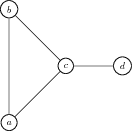
\includegraphics[width=0.5\linewidth]{images/degreeexamplegraph.png}
\caption{The graph \(K\)\label{fig_trumpet_graph}}
\end{figure}
\hypertarget{p-20}{}%
In the graph \(K\) shown in \hyperref[fig_trumpet_graph]{Figure~\ref{fig_trumpet_graph}}, vertices \(a\) and \(b\) have degree 2, vertex \(c\) has degree 3, and vertex \(d\) has degree 1.%
\end{example}
\hypertarget{p-21}{}%
Note that in the definition we require \(G\) to be a simple graph.  The notion of degree has a few pitfalls to be careful of \(G\) has loops or multiple edges.  We still want to the degree \(d(v)\) to match the intuitive notion of the ``number of edges coming out of \(v\)'' captured in the drawing with a small circle.  The trap to beware is that this notion no longer agrees with ``the number of vertices adjacent to \(v\)'' or the ``the number of edges incident to \(v\)''%
\begin{example}[]\label{example-4}
\end{example}
\typeout{************************************************}
\typeout{Subsection 1.2.2 Extended example: Chemistry}
\typeout{************************************************}
\subsection[{Extended example: Chemistry}]{Extended example: Chemistry}\label{subsection-5}
\hypertarget{p-22}{}%
In organic chemistry, molecules are frequently drawn as graphs, with the vertices being atoms, and an edge betwen two vertices if and only if the corresponding atoms have a covalent bond between them (that is, they share a vertex).%
\begin{example}[Alkanes]\label{example-5}
\end{example}
\hypertarget{p-23}{}%
The location of an element on the periodic table determines the valency of the element -- hence the degree that vertex has in any molecule containing that graph:%
\leavevmode%
\begin{itemize}[label=\textbullet]
\item{}Hydrogen (H) and Fluorine (F) have degree 1%
\item{}Oxygen (O) and Sulfur (S) have degree 2%
\item{}Nitrogen (N) and Phosphorous (P) have degree 3%
\item{}Carbon (C) has degree 4%
\end{itemize}
\hypertarget{p-24}{}%
Usually, most of the atoms involved are carbon and hydrogen. Carbon atoms are not labelled with a C, but just left blank, while hydrogen atoms are left off completely. One can then complete the full structure of the molecule using the valency of each vertex.  On the exam, you may have to know that Carbon has degree 4 and Hydrogen has degree 1; the valency of any other atom would be provided to you%
\par
\hypertarget{p-25}{}%
Graphs coming from organic chemistry do not have to be simple – sometimes there are double bonds, where a pair of carbon atoms have two edges between them.%
\begin{example}[]\label{example-6}
\end{example}
\hypertarget{p-26}{}%
If we know the chemical formula of a molecule, then we know how many vertices of each degree it has.  For a general graph, this information is known as the degree sequence%
\begin{definition}[{Degree sequence}]\label{definition-7}
\hypertarget{p-27}{}%
The degree sequence of a graph is just the list (with multiplicity) of the degrees of all the vertices.%
\end{definition}
\hypertarget{p-28}{}%
The following sage code draws a random graph with 7 vertices and 10 edges, and then gives its degree sequence.  You can tweak the code to generate graphs with different number of vertices and edges, and run the code multiple times, and the degree sequence should become clear.%
\begin{sageinput}
vertices = 7
edges = 10
g = graphs.RandomGNM(vertices,edges)
g.show()
print g.degree_sequence()
\end{sageinput}
\hypertarget{p-29}{}%
Knowing the chemical composition of a molecule determines the degree sequence of its corresponding graph. However, it is possible that the same set of atoms may be put together into a molecule in more than one different ways. In chemistry, these are called \emph{isomers}.  In terms of graphs, this corresponds to different graphs that have the same degree sequence.%
\par
\hypertarget{p-30}{}%
An important special case is the constant degree sequence.%
\begin{definition}[{Regular graphs}]\label{definition-8}
\hypertarget{p-31}{}%
A graph \(\Gamma\) is \(d\)-\emph{regular}, or \emph{regular of degree} \(d\) if every vertex \(v\in\Gamma\) has the same degree \(d\), i.e. \(d(v)=d\).%
\end{definition}
\hypertarget{p-32}{}%
As a common special case, a regular graph where every vertex has degree three is called \emph{trivalent}, or \emph{cubic}.%
\par
\hypertarget{p-33}{}%
Some quick examples: \leavevmode%
\begin{enumerate}
\item\hypertarget{li-8}{}The cycle graph \(C_n\) is two-regular%
\item\hypertarget{li-9}{}The complete graph \(K_n\) is \((n-1)\)-regular%
\item\hypertarget{li-10}{}The Petersen graph is trivalent%
\end{enumerate}
%
\begin{exercise}\label{exercise-1}
\end{exercise}
\typeout{************************************************}
\typeout{Subsection 1.2.3 Handshaking lemma and first applications}
\typeout{************************************************}
\subsection[{Handshaking lemma and first applications}]{Handshaking lemma and first applications}\label{subsection-6}
\begin{theorem}[{}]\label{theorem-1}
\hypertarget{p-35}{}%
(Euler's handshaking Lemma)%
%
\begin{equation*}
\sum_{v\in V(G)}d(v)=2|E(G)|
\end{equation*}
\end{theorem}
\begin{proof}\hypertarget{proof-1}{}
\hypertarget{p-36}{}%
We count the ``ends'' of edges two different ways.  On the one hand, every end occurs at a vertex, and at vertex \(v\) there are \(d(v)\) ends, and so the total number of ends is the sum on the left hand side. On the other hand, every edge has exactly two ends, and so the number of ends is twice the number of edges, giving the right hand side.%
\end{proof}
\hypertarget{p-37}{}%
Euler's handshaking lemma will be particularly useful in Section 3, when we study graphs on surfaces, but already it still has some amusing corollaries.%
\typeout{************************************************}
\typeout{Section 1.3 Graph Isomorphisms}
\typeout{************************************************}
\section[{Graph Isomorphisms}]{Graph Isomorphisms}\label{s_intro_isomorphisms}
\hypertarget{p-38}{}%
Generally speaking in mathematics, we say that two objects are "isomorphic" if they are "the same" in terms of whatever structure we happen to be studying.  The symmetric group \(S_3\) and the symmetry group of an equilateral triangle \(D_6\) are isomorphic.  In this section we briefly briefly discuss isomorphisms of graphs.%
\typeout{************************************************}
\typeout{Subsection 1.3.1 Isomorphic graphs}
\typeout{************************************************}
\subsection[{Isomorphic graphs}]{Isomorphic graphs}\label{subsection-7}
\hypertarget{p-39}{}%
It is possible to draw the same graph in the plane in many different ways – e.g., the pentagon \(C_5\), and its complement the five sided star \(C_5^c\) are actually "the same", as indicated by the following labeling of the vertices:%
\begin{definition}[{}]\label{definition-9}
\hypertarget{p-40}{}%
An isomorphism \(\varphi:G\to H\) of simple graphs is a biject \(\varphi:V(G)\to V(H)\) between their vertex sets that preserves the number of edges between vertices.  In other words, \(\varphi(v)\) and \(\varphi(w)\) are adjacent in \(H\) if and only if \(v\) and \(w\) are adjancent in \(G\).%
\end{definition}
\begin{example}[]\label{example-7}
\hypertarget{p-41}{}%
This animated gif shows several graphs isomorphic to the Petersen graph, and demonstrates that they are isomorphic.%
\includegraphics[width=1\linewidth]{images/PetersenIsomorphismAnimated.gif}
\hypertarget{p-42}{}%
Animated gif by \href{https://msollami.com/code/2014/12/24/graph-isomorphisms}{Michael Sollami} for \href{https://www.quantamagazine.org/algorithm-solves-graph-isomorphism-in-record-time-20151214/}{this Quanta Magazine article} on the Graph Isomorphism problem%
\end{example}
\begin{example}[]\label{example-8}
\leavevmode%
\begin{figure}
\centering
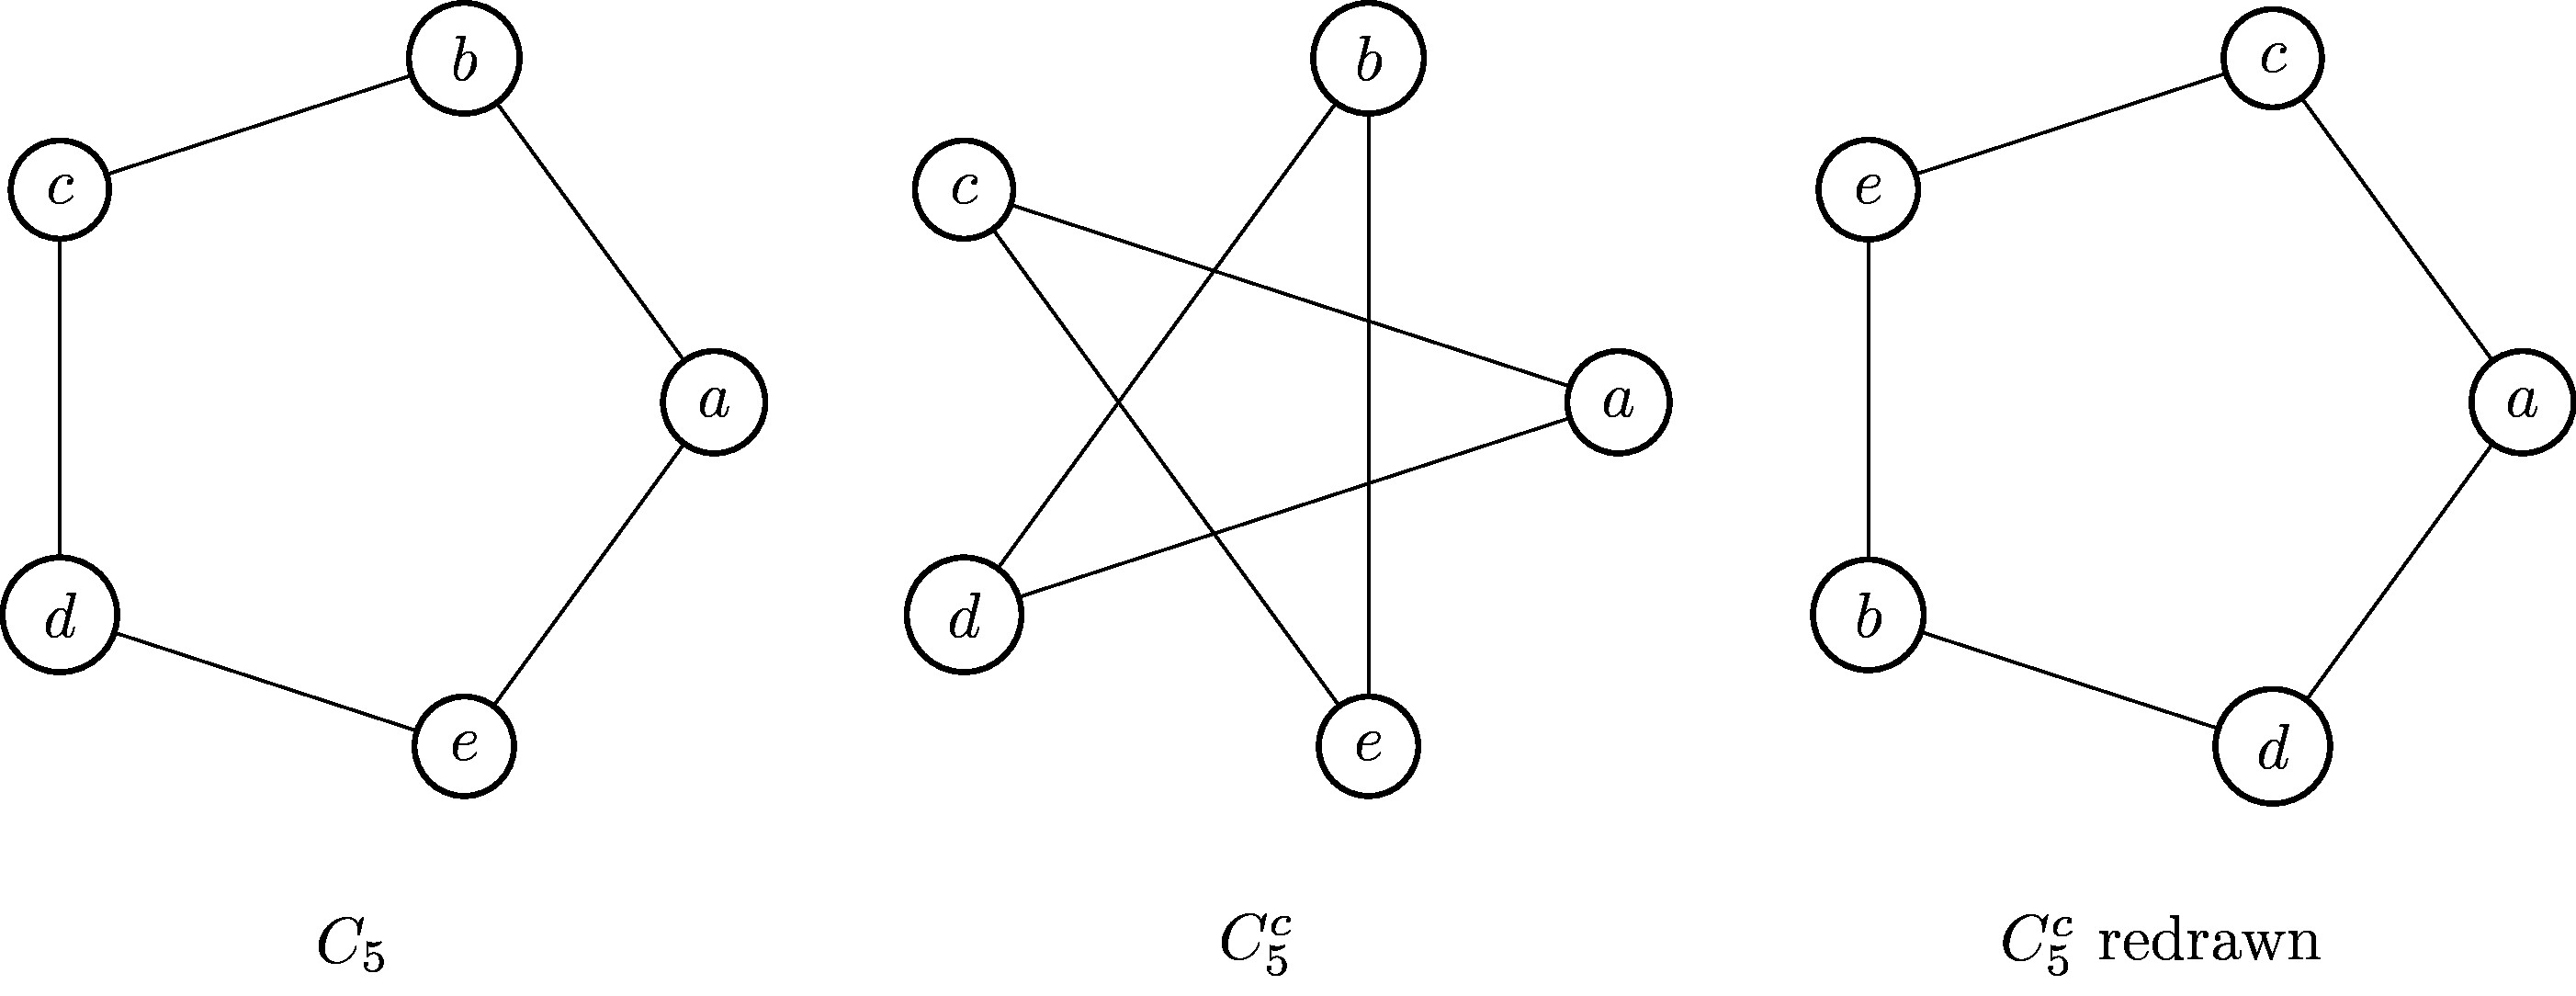
\includegraphics[width=0.9\linewidth]{images/cycleandstar.jpg}
\caption{\(C_5\) is isomorphic to its complement \(C_5^c\)\label{figure-2}}
\end{figure}
\hypertarget{p-43}{}%
The cycle graph on 5 vertices, \(C_5\) is isomorphic to its complement, \(C_5^c\).  The cycle \(C_5\) is usually drawn as a pentagon, and if we were then going to naively draw \(C_5^c\) we would draw a 5-sided star.  However, we could draw \(C_5^c\) differently as shown, making it clear that it is isomorphic to \(C_5\), with isomorphism \(\varphi:C_5\to C_5^c\) defined by \(\varphi(a)=a, \varphi(b)=c, \varphi(c)=e, \varphi(d)=b, \varphi(e)=d\).%
\end{example}
\hypertarget{p-44}{}%
Although solving the graph isomorphism problem for general graphs is quite difficult, doing it for small graphs by hand is not too bad and is something you must be able to do for the exam.  If the two graphs are actually isomorphic, then you should show this by exhibiting an isomrophism; that is, writing down an explicit bijection between their vertex sets with the desired properties. The most attractive way of doing this, for humans, is to label the vertices of both copies with the same letter set.%
\par
\hypertarget{p-45}{}%
If two graphs are not isomorphic, then you have to be able to prove that they aren't. Of course, one can do this by exhaustively describing the possibilities, but usually it's easier to do this by giving an obstruction – something that is different between the two graphs. One easy example is that isomorphic graphs have to have the same number of edges and vertices. We'll discuss some others in the next section%
\typeout{************************************************}
\typeout{Subsection 1.3.2 Heuristics for showing graphs are or aren't isomorphic}
\typeout{************************************************}
\subsection[{Heuristics for showing graphs are or aren't isomorphic}]{Heuristics for showing graphs are or aren't isomorphic}\label{subsection-8}
\hypertarget{p-46}{}%
Another, only slightly more advanced invariant is the degree sequence of a graph that we saw last lecture in our discussion of chemistry.%
\par
\hypertarget{p-47}{}%
If \(\varphi:G\to H\) is an isomorphism of graphs, than we must have \(d(\varphi(v))=d(v)\) for all vertices \(v\in G\), and since isomorphisms are bijections on the vertex set, we see the degree sequence must be preserved.  However, just because two graphs have the same degree sequences does not mean they are isomorphic.%
\par
\hypertarget{p-48}{}%
Slightly subtler invariants are number and length of cycles and paths.%
\typeout{************************************************}
\typeout{Subsection 1.3.3 Cultural Literacy: The Graph Isomorphism Problem}
\typeout{************************************************}
\subsection[{Cultural Literacy: The Graph Isomorphism Problem}]{Cultural Literacy: The Graph Isomorphism Problem}\label{subsection-9}
\hypertarget{p-49}{}%
This section, as all "Cultural Literacy" sections, is information that you may find interesting, but won't be examined.%
\par
\hypertarget{p-50}{}%
The graph isomorphism problem is the following: given two graphs \(G\) and \(H\), determine whether or not \(G\) and \(H\) are isomorphic. Clearly, for any two graphs \(G\) and \(H\), the problem is solvable: if \(G\) and \(H\) both of \(n\) vertices, then there are \(n!\) different bijections between their vertex sets.  One could simply examine each vertex bijection in turn, checking whether or not it maps edges to edges.%
\par
\hypertarget{p-51}{}%
The problem is interesting because the naive algorithm discussed above is not very efficient: for large \(n\), \(n!\) is absolutely huge, and so in general this algorithm will take a long time.  The question is, is there are a faster way to do check? How fast can we get?%
\par
\hypertarget{p-52}{}%
The isomorphism problem is of fundamental importance to theoretical computer science. Apart from its practical applications, the exact difficulty of the problem is unknown. Clearly, if the graphs are isomorphic, this fact can be easily demonstrated and checked, which means the Graph Isomorphism is in NP.%
\par
\hypertarget{p-53}{}%
Most problems in NP are known either to be easy (solvable in polynomial time, P), or at least as difficult as any other problem in NP (NP complete). This is not true of the Graph Isomorphism problem. In November of last year, Laszlo Babai announced a quasipolynomial-time algorithm for the graph isomorphism problem – you can read about this work in this great popular science article.%
\typeout{************************************************}
\typeout{Section 1.4 Instant Insanity}
\typeout{************************************************}
\section[{Instant Insanity}]{Instant Insanity}\label{s_intro_instantinsanity}
\hypertarget{p-54}{}%
So far, our motivation for studying graph theory has largely been one of philosophy and language.  Before we get too much deeper, however, it may be useful to present a nontrivial and perhaps unexpected application of graph theory; an example where graph theory helps us to do something that would be difficult or impossible to do without it.%
\typeout{************************************************}
\typeout{Subsection 1.4.1 A puzzle}
\typeout{************************************************}
\subsection[{A puzzle}]{A puzzle}\label{subsection-10}
\leavevmode%
\begin{figure}
\centering

\includegraphics[width=0.8\linewidth]{images/InstantInsanityPackage.JPG}
\caption{Instant Insanity Package\label{figure-3}}
\end{figure}
\hypertarget{p-55}{}%
There is a puazzle marketed under the name "Instant Insanity", one version of which is shown above.  The puzzle is sometimes called "the four cubes problem", as it consists of four different cubes.   Each face of each cube is painted one of four different colours: blue, green, red or yellow. The goal of the puzzle is to line the four cubes up in a row, so that along the four long edges (front, top, back, bottom) each of the four colours appears eactly once.%
\par
\hypertarget{p-56}{}%
Depending on how the cubes are coloured, this may be not be possible, or there may be many such possibilities. In the original instant insanity, there is exactly one solution (up to certain equivalences of cube positions).  The point of the cubes is that there are a large number of possible cube configurations, and so if you just look for a solution without being extremely systematic, it is highly unlikely you will find it.%
\par
\hypertarget{p-57}{}%
But trying to be systematic and logical about the search directly is quite difficult, perhaps because we have problems holding the picture of the cube in our mind.  In what follows, we will introduce a way to translate the instant insanity puzzle into a question in graph theory.  This is obviously in no way necessary to solve the puzzle, but does make it much easier.  It also demonstrates the real power of graph theory as a visualization and thought aid.%
\begin{exercise}\label{exercise-2}
\end{exercise}
\hypertarget{p-59}{}%
There are many variations on Instant Insanity, discussions of which can be found \href{http://www.cs.brandeis.edu/\~storer/JimPuzzles/ZPAGES/zzzInstantInsanity.html}{here} and \href{http://www.jaapsch.net/puzzles/insanity.htm}{here}. There’s also a \href{https://www.youtube.com/watch?v=CQ2gHSKZBEw}{commercial} for the game.%
\typeout{************************************************}
\typeout{Subsection 1.4.2 Enter graph theory}
\typeout{************************************************}
\subsection[{Enter graph theory}]{Enter graph theory}\label{subsection-11}
\hypertarget{p-60}{}%
It turns out that the important factor of the cubes is what color is on the opposite side of each face.  Suppose we want face one facing forward.  Then we have four different ways to rotate the cube to keep this the same.  The same face will always appear on the opposite side, but we can get any of the remaining four faces to be on top, say.%
\begin{figure}
\centering
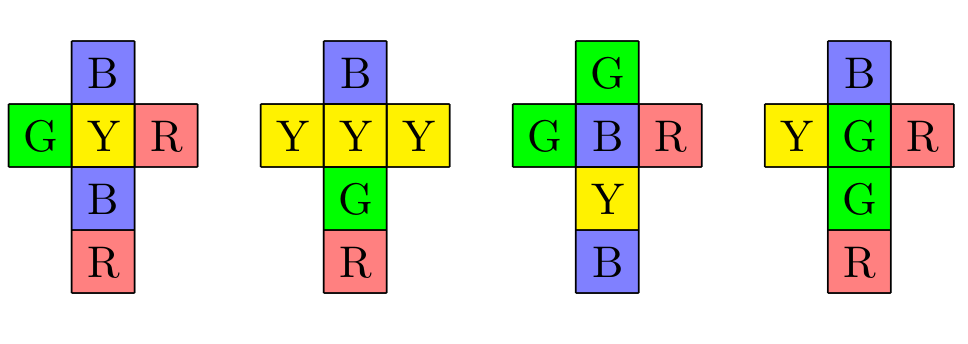
\includegraphics[width=1\linewidth]{images/ImpossibleCubes.png}
\caption{An impossible set of cubes\label{fig_impossible_cubes}}
\end{figure}
\hypertarget{p-61}{}%
Let us encode this information in a graph.   The vertices of the graph will be the four colors, B, G, R and Y. We will put an edge between two colors each time they appear as opposite faces on a cube, and we will label that edge with a number 1-4 denoting which cube the two opposite faces appear. Thus, in the end the graph will have twelve edges, three with each label 1-4. For from the first cube, there will be a loop at B, and edge between G and R, and an edge between Y and R.  The graph corresponding to the four cubes above is the following:%
\begin{figure}
\centering
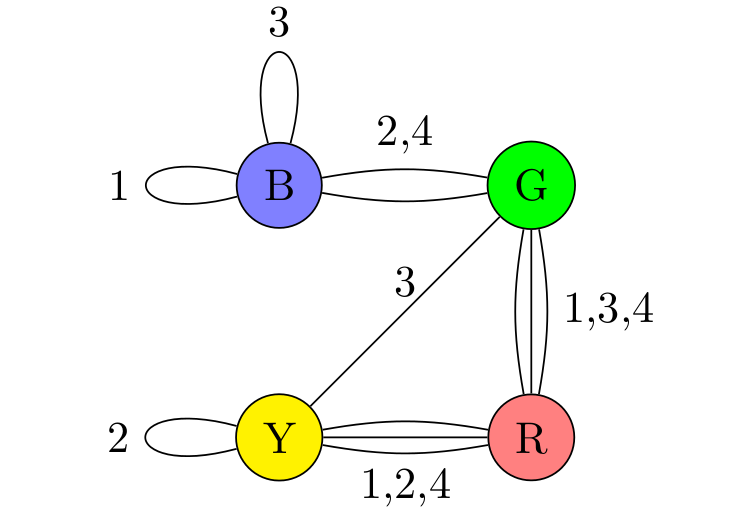
\includegraphics[width=0.9\linewidth]{images/InstantInsanityImpossibleGraph.png}
\caption{The graph constructed from the cubes in \hyperref[fig_impossible_cubes]{Figure~\ref{fig_impossible_cubes}}\label{fig_graph_from_cubes}}
\end{figure}
\typeout{************************************************}
\typeout{Subsection 1.4.3 Proving that our cubes were impossible}
\typeout{************************************************}
\subsection[{Proving that our cubes were impossible}]{Proving that our cubes were impossible}\label{subsection-12}
\hypertarget{p-62}{}%
We now analyze the graph to prove that this set of cubes is not possible.%
\par
\hypertarget{p-63}{}%
Suppose we had an arrangement of the cubes that was a solution. Then, from each cube, pick the edge representing the colors facing front and back on that cube. These four edges are a subgraph of our original graph, with one edge of each label, since we picked one edge from each cube. Furthermore, since we assumed the arrangement of cubes was a solution of instant insanity, each color appears once on the front face and once on the back. In terms of our subgraph, this translates into asking that each vertex has degree two.%
\par
\hypertarget{p-64}{}%
We can get another subgraph satisfying these two properties by looking at the faces on the top and bottom for each cube and taking the corresponding edges. Furthermore, these two subgraphs do not have any edges in common.%
\par
\hypertarget{p-65}{}%
Thus, given a solution to the instant insanity problem, we found a pair of subgraphs \(S_1, S_2\) satisfying: \leavevmode%
\begin{enumerate}
\item\hypertarget{li-11}{}Each subgraph \(S_i\) has one edge with each label 1,2,3,4%
\item\hypertarget{li-12}{}Every vertex of \(S_i\) has degree 2%
\item\hypertarget{li-13}{}No edge of the original graph is used in both \(S_1\) and \(S_2\)%
\end{enumerate}
 As an exercise, one can check that given a pair of subgraphs satisfying 1-3, one can produce a solution to the instant insanity puzzle.%
\par
\hypertarget{p-66}{}%
Thus, to show the set of cubes we are currently examining does not have a solution, we need to show that the graph does not have two subgraphs satisfying properties 1-3.%
\par
\hypertarget{p-67}{}%
To do, this, we catalog all graphs satisfying properties 1-2. If every vertex has degree 2, either: \leavevmode%
\begin{enumerate}
\item\hypertarget{li-14}{}Every vertex has a loop%
\item\hypertarget{li-15}{}There is one vertex with a loop, and the rest are in a triangle%
\item\hypertarget{li-16}{}There are two vertices with loops and a double edge between the other two vertices%
\item\hypertarget{li-17}{}There are two pairs of double edges%
\item\hypertarget{li-18}{}All the vertices live in one four cycle%
\item\hypertarget{li-19}{}A subgraphs of type 1 is not possible, because G and R do not have loops.%
\end{enumerate}
%
\par
\hypertarget{p-68}{}%
For subgraphs of type 2, the only triangle is G-R-Y, and B does have loops. The edge between Y-G must be labeled 3, which means the loop at B must be labeled 1. This means the edge between G and R must be labeled 4 and the edge between Y and R must be 2, giving the following subgraph:%
\begin{figure}
\centering
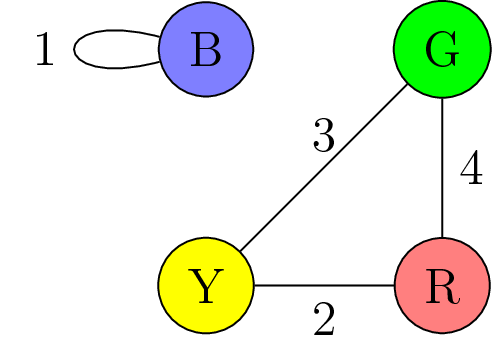
\includegraphics[width=0.4\linewidth]{images/InstantInsanityImpossibleFirst.png}
\caption{A subgraph for a solution for one pair of faces\label{fig_impossible_first}}
\end{figure}
\hypertarget{p-69}{}%
For type 3, the only option is to have loops at B and Y and a double edge between G and R. We see the loop at Y must be labeled 2, one of the edges between G and R must be 4, and the loop at B and the other edge between G and R can switch between 1 and 3, giving two possibilities:%
\begin{figure}
\centering
% group protects changes to lengths, releases boxes (?)
{% begin: group for a single side-by-side
% set panel max height to practical minimum, created in preamble
\setlength{\panelmax}{0pt}
\ifdefined\panelboxAimage\else\newsavebox{\panelboxAimage}\fi%
\begin{lrbox}{\panelboxAimage}
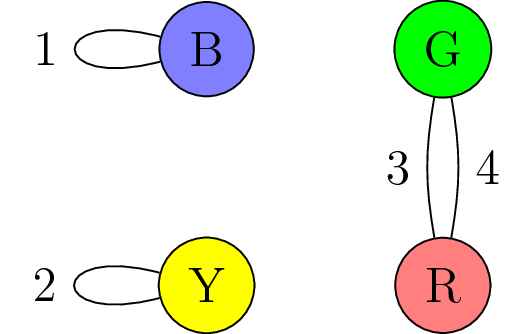
\includegraphics[width=0.4\linewidth]{images/InstantInsanityImpossibleSecond.png}
\end{lrbox}
\ifdefined\phAimage\else\newlength{\phAimage}\fi%
\setlength{\phAimage}{\ht\panelboxAimage+\dp\panelboxAimage}
\settototalheight{\phAimage}{\usebox{\panelboxAimage}}
\setlength{\panelmax}{\maxof{\panelmax}{\phAimage}}
\ifdefined\panelboxBimage\else\newsavebox{\panelboxBimage}\fi%
\begin{lrbox}{\panelboxBimage}
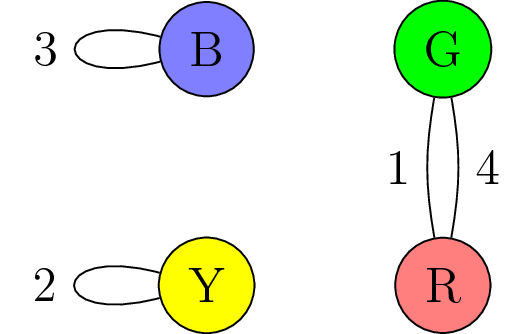
\includegraphics[width=0.4\linewidth]{images/InstantInsanityImpossibleThird.png}
\end{lrbox}
\ifdefined\phBimage\else\newlength{\phBimage}\fi%
\setlength{\phBimage}{\ht\panelboxBimage+\dp\panelboxBimage}
\settototalheight{\phBimage}{\usebox{\panelboxBimage}}
\setlength{\panelmax}{\maxof{\panelmax}{\phBimage}}
\leavevmode%
% begin: side-by-side as tabular
% \tabcolsep change local to group
\setlength{\tabcolsep}{0.05\linewidth}
% @{} suppress \tabcolsep at extremes, so margins behave as intended
\par\medskip\noindent
\hspace*{0.05\linewidth}%
\begin{tabular}{@{}*{2}{c}@{}}
\begin{minipage}[c][\panelmax][c]{0.4\linewidth}\usebox{\panelboxAimage}\end{minipage}&
\begin{minipage}[c][\panelmax][c]{0.4\linewidth}\usebox{\panelboxBimage}\end{minipage}\end{tabular}\\
% end: side-by-side as tabular
}% end: group for a single side-by-side
\caption{Two more subgraphs for a partial solutions\label{fig_impossible_twoandthree}}
\end{figure}
\hypertarget{p-70}{}%
For subgraphs of type 4, the only option would be to have a double edge between B and G and another between Y and R; however, none of these edges are labeled 3 and this option is not possible.%
\par
\hypertarget{p-71}{}%
Finally, subgraphs of type 5 cannot happen because B is only adjacent to G and to itself; to be in a four cycle it would have two be adjacent to two vertices that aren’t itself.%
\par
\hypertarget{p-72}{}%
This gives three different possibilities for the subgraphs SiSi that satisfy properties 1 and 2. However, all three possibilities contain the the edge labeled 4 between G and R; hence we cannot choice two of them with disjoint edges, and the instant insanity puzzle with these cubes does not have a solution.%
\typeout{************************************************}
\typeout{Subsection 1.4.4 Other cube sets}
\typeout{************************************************}
\subsection[{Other cube sets}]{Other cube sets}\label{subsection-13}
\hypertarget{p-73}{}%
The methods above also give a way to find the solution to a set of instant insanity cubes should one exist.  I illustrate this in the following Youtube video:%
\begin{tabular}{m{.2\linewidth}m{.6\linewidth}}
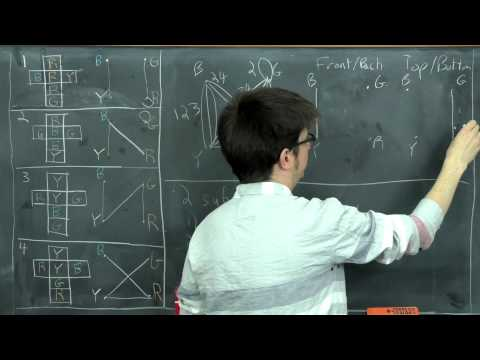
\includegraphics[width=\linewidth]{images/video-1.jpg}&%
Other cube sets\newline%
\href{https://www.youtube.com/watch?v=GsbhRfjaaN8}{\texttt{\nolinkurl{www.youtube.com/watch?v=GsbhRfjaaN8}}}
\end{tabular}
\typeout{************************************************}
\typeout{Exercises 1.5 Exercises}
\typeout{************************************************}
\section[{Exercises}]{Exercises}\label{s_intro_exercises}
\begin{exerciselist}
\item[1.]\hypertarget{exercise-3}{}\hypertarget{p-74}{}%
For each of the following sequences, either give an example of such a graph, or explain why one does not exist.%
\leavevmode%
\begin{enumerate}[label=(\alph*)]
\item\hypertarget{li-20}{}\hypertarget{p-75}{}%
A graph with six vertices whose degree sequence is \([5,5,4,3,2,2]\)%
\item\hypertarget{li-21}{}\hypertarget{p-76}{}%
A graph with six vertices whose degree sequence is \([5,5,4,3,3,2]\)%
\item\hypertarget{li-22}{}\hypertarget{p-77}{}%
A graph with six vertices whose degree sequence is \([5,5,5,5,3,3]\)%
\item\hypertarget{li-23}{}\hypertarget{p-78}{}%
A simple graph with six vertices whose degree sequence is \([5,5,5,5,3,3]\)%
\end{enumerate}
\par\smallskip
\item[2.]\hypertarget{exercise-4}{}\hypertarget{p-79}{}%
For the next Olympic Winter Games, the organizers wish to expand the number of teams competing in curling. They wish to have \(14\) teams enter, divided into two pools of seven teams each. Right now, they're thinking of requiring that in preliminary play each team will play seven games against distinct opponents. Five of the opponents will come from their own pool and two of the opponents will come from the other pool. They're having trouble setting up such a schedule, so they've come to you. By using an appropriate graph-theoretic model, either argue that they cannot use their current plan or devise a way for them to do so.%
\par\smallskip
\item[3.]\hypertarget{exercise-5}{}\hypertarget{p-80}{}%
\hyperref[isomorphic_exercise]{Figure~\ref{isomorphic_exercise}} contains four graphs on six vertices. Determine which (if any) pairs of graphs are isomorphic. For pairs that are isomorphic, give an isomorphism between the two graphs. For pairs that are not isomorphic, explain why.%
\begin{figure}
\centering
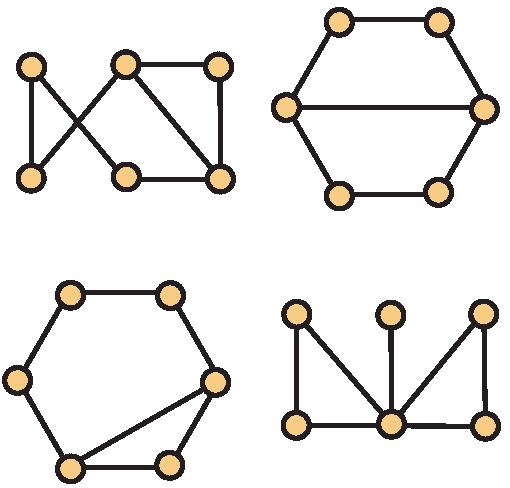
\includegraphics[width=0.55\linewidth]{images/isomorphic_ex}
\caption{Are these graphs isomorphic?\label{isomorphic_exercise}}
\end{figure}
\par\smallskip
\item[4.]\hypertarget{exercise-6}{}\hypertarget{p-81}{}%
Recall that \(G^c\) denotes the complement of a graph \(G\).  Prove that \(f:G\to H\) is an isomorphism of graphs if and only if \(f:G^c\to H^c\) is an isomorphism.%
\par\smallskip
\item[5.]\hypertarget{exercise-7}{}\hypertarget{p-82}{}%
Determine the number of non-isomorphic simple graphs with seven vertices such that each vertex has degree at least five.%
\par\smallskip
\par\smallskip%
\noindent\textbf{Hint.}\hypertarget{hint-1}{}\quad%
\hypertarget{p-83}{}%
Consider the previous exercise%
\end{exerciselist}
\typeout{************************************************}
\typeout{Chapter 2 Walks}
\typeout{************************************************}
\chapter[{Walks}]{Walks}\label{ch_walks}
\hypertarget{p-84}{}%
In this chapter we investigate walks in graphs.  We first look at some basic definitions and examples, we discuss Dijkstra's algorithm for finding the shortest path between two points in a weighted graph, and we discuss the notions of Eulerian and Hamiltonian graphs.%
\typeout{************************************************}
\typeout{Section 2.1 Walks: the basics}
\typeout{************************************************}
\section[{Walks: the basics}]{Walks: the basics}\label{s_walks_basics}
\hypertarget{p-85}{}%
If the edges in a graph \(\Gamma\) represent connections between different cities, it is obvious to strart planning longer trips that compose several of these connections.  The notion of a \emph{walk} formally captures this definition; the formal notions of \emph{path} and \emph{trail} further ask that we not double back on ourselves or repeat ourselves in certain formally defined ways.%
 \par
\hypertarget{p-86}{}%
Once we've done that, we investigate what it means for a graph to be connected or disconnected.%
\typeout{************************************************}
\typeout{Subsection 2.1.1 Walks and connectedness}
\typeout{************************************************}
\subsection[{Walks and connectedness}]{Walks and connectedness}\label{subsection-14}
\hypertarget{p-87}{}%
Before we see the formal definition of a walk, it will be useful to see an example:%
\begin{figure}
\centering
{
\begin{tikzpicture}
\begin{scope}[every node/.style={circle,thick,draw}]
    \node (A) at (0,0) {A};
    \node (B) at (0,3) {B};
    \node (C) at (2.5,4) {C};
    \node (D) at (2.5,1) {D};
    \node (E) at (2.5,-3) {E};
    \node (F) at (5,3) {F} ;
\end{scope}

\begin{scope}[every node/.style={fill=white,circle}, >={Stealth[black]}]
  \begin{scope}[            
              every edge/.style={draw=red,very thick}]

  \path [->] (A) edge node {$6$} (D);
 \path [->] (D) edge node {$4$} (C);
    \path [->] (C) edge node {$5$} (F);
    \path [->] (F) edge node {$3$} (D);
    \path [->] (D) edge node {$8$} (E);
\end{scope}
    
    \path  (A) edge node {$3$} (B);
    \path  (B) edge node {$1$} (C); 
    \path  (A) edge node {$7$} (E);
    \path  (E) edge node {$9$} (F); 
    \path  (B) edge[bend right=60] node {$10$} (E); 
\end{scope}
\end{tikzpicture}
}
\caption{Example of a walk\label{fig_walkdrawing}}
\end{figure}
\hypertarget{p-88}{}%
In the graph shown, the vertices are labelled with letters, and the edges are labelled with numbers, and we have a walk highlighted in red, and with arrowtips drawn on the edges.  Starting from vertex \(A\), we can take edge 6 to vertex \(D\), and then edge 5 to vertex \(C\), edge 5 to vertext \(F\), edge 3 back to vertex \(D\), and finally edge 8 to vertex \(E\). Intuitively,then, a walk strings together several edges that share vertices in between.  Makign that formal, we have the following.%
\begin{definition}[{Walk}]\label{definition-10}
\hypertarget{p-89}{}%
\(walk\) in a graph \(\Gamma\) is a sequence%
%
\begin{equation*}
v_0, e_1, v_1,e_2, v_2,\dots, v_{n-1}, e_n, v_n
\end{equation*}
\hypertarget{p-90}{}%
where the \(v_i\) are vertices, the \(e_j\) are edges, and the edge \(e_j\) goes between vertices \(v_{j-1}\) and \(v_j\).%
\par
\hypertarget{p-91}{}%
We say that the walk is between vertices \(a=v_0\) and \(b=v_n\)%
\end{definition}
\hypertarget{p-92}{}%
With this notation for a walk, Example \hyperref[fig_walkdrawing]{Figure~\ref{fig_walkdrawing}}, the walk shown would be written \(A, 6, D, 4, C, 5, F, 3, D, 8, E\).  The visual representation of the walk on the graph is vastly more intuitive, the written one feeling cumbersome in comparison.%
\par
\hypertarget{p-93}{}%
The definition of walk above contains some extra information.  If we just know the sequence of edges we can reconstruct what the vertices have to be (assuming we have at least two edges in the walk).  Alternatively, if the graph \(\Gamma\) does not have multiple edges, it is enough to just know the vertices \(v_i\), but if \(\Gamma\) has multiple edges that just knowing the vertices does not determine the walk.%
\begin{definition}[{Connected}]\label{definition-11}
\hypertarget{p-94}{}%
We say a graph \(\Gamma\) is \emph{connected} if for any two vertices \(v,w\), there is a walk from \(v\) to \(w\) in \(\Gamma\).%
\end{definition}
\begin{definition}[{Disjoint union}]\label{definition-12}
\hypertarget{p-95}{}%
Given two graphs \(\Gamma_1\) and \(\Gamma_2\), the \emph{disjoint union} \(\Gamma_1\sqcup \Gamma_2\) is obtained by taking the disjoint union of both the vertices and edges of \(\Gamma_1\) and \(\Gamma_2\).  So \(\Gamma_1\sqcup\Gamma_2\) consists of a copy of \(\Gamma_1\) and a copy of \(\Gamma_2\), with no edges in between the two graphs.%
\end{definition}
\begin{definition}[{Disconnected}]\label{definition-13}
\hypertarget{p-96}{}%
A graph \(\Gamma\) is \emph{disconnected} if we can write \(\Gamma=\Gamma_1\sqcup \Gamma_2\) for two proper (i.e., not all of \(\Gamma\)) subgraphs \(\Gamma_1\) and \(\Gamma_2\).%
\end{definition}
\hypertarget{p-97}{}%
We now have a definition for what it means for a graph to be connected, and another for what it means for a graph to be disconnected.  From everday usage of this words, we would certainly hope that a graph is disconnected if and only if it is not connected.  However, it is not immediately clear from the definitions as written that this is the case.%
\begin{lemma}[{}]\label{lemma-1}
\hypertarget{p-98}{}%
The following are equivalent:%
\leavevmode%
\begin{enumerate}
\item\hypertarget{li-24}{}. \(\Gamma\) is connected%
\item\hypertarget{li-25}{}\(\Gamma\) is not disconnected%
\end{enumerate}
\end{lemma}
\begin{proof}\hypertarget{proof-2}{}
\hypertarget{p-99}{}%
1 implies 2: Supppose that \(\Gamma\) is connected, and let \(v, w\in V(\Gamma)\); we want to show that there is a walk from \(v\) to \(w\).%
\par
\hypertarget{p-100}{}%
Define \(S\subset V(\Gamma)\) to be the set of all vertices \(u\in V(\Gamma)\) so that there is a walk from \(v\) to \(u\); we want to show that \(w\in S\).%
\par
\hypertarget{p-101}{}%
First, observe that there are no edges from \(S\) to \(V(\Gamma)\setminus S\).  Suppose that \(e\) was an edge between \(a\in S\) and \(b\in\Gamma\setminus S\).  Since \(a\in S\), by the definition of \(S\) there is a walk \(v=v_0v_1v_2\cdots v_m=a\) from \(v\) to \(a\).  We can add the edge \(e\) to the end of the walk, to get a walk from \(v\) to \(b\), and hence by definition \(b\in S\).%
\par
\hypertarget{p-102}{}%
Now suppose that \(w\notin S\).  Then \(S\) and \(V(\Gamma)\setminus S\) are both nonempty, and by the above there are no edges between them, and so \(\Gamma\) is not connected, a contradiction.%
\par
\hypertarget{p-103}{}%
To prove 2 implies 1, we prove the contrapositive.  If \(\Gamma\) is not connected, then there are two vertices \(v,w\in V(\Gamma)\) so that there is no walk from \(v\) to \(w\).%
\par
\hypertarget{p-104}{}%
Suppose that \(\Gamma=\Gamma_1\sqcup\Gamma_2\), and pick \(v\in V(\Gamma_1), w\in V(\Gamma_2)\).  Any walk from \(v\) to \(w\) starts in \(V(\Gamma_1)\) and ends in \(V(\Gamma_2)\), and so at some point there must be an edge from a vertex in \(\Gamma_1\) to a vertex in \(\Gamma_2\), but there are no such edges \(\square\)%
\end{proof}
\typeout{************************************************}
\typeout{Subsection 2.1.2 Types of Walks}
\typeout{************************************************}
\subsection[{Types of Walks}]{Types of Walks}\label{subsection-15}
\hypertarget{p-105}{}%
Many questions in graph theory ask whether or not a walk of a certain type exists on a graph: we introduce some notation that will be needed for these questions.%
\begin{definition}[{}]\label{definition-14}
\hypertarget{p-106}{}%
We say a walk is \emph{closed} if it starts and ends on the same vertex; i.e., \(v_0=v_n\).  The \emph{length} of a walk is \(n\), the number of edges in it.  The \emph{distance} between two vertices \(v\) and \(w\) is the length of the shortest walk from \(v\) to \(w\), if one exists, and \(\infty\) if one does not exist.%
\end{definition}
\hypertarget{p-107}{}%
It is sometimes convenient to have terminology for walks that don't backtrack on themselves:%
\begin{definition}[{}]\label{definition-15}
\leavevmode%
\begin{enumerate}
\item\hypertarget{li-26}{}If the edges \(e_i\) of the walk are all distinct, we call it a \emph{trail}%
\item\hypertarget{li-27}{}If the vertices \(v_i\) of the walk are all distinct (except possibly \(v_0=v_m\)), we call the walk a \emph{path}.  The exception is to allow for the possibility of closed paths.%
\end{enumerate}
\end{definition}
\begin{lemma}[{}]\label{lemma-2}
\hypertarget{p-108}{}%
Let \(v,w\in V(\Gamma)\).  The following are equivalent:%
\leavevmode%
\begin{enumerate}
\item\hypertarget{li-28}{}There is a walk from \(v\) to \(w\)%
\item\hypertarget{li-29}{}There is a trail from \(v\) to \(w\)%
\item\hypertarget{li-30}{}There is a path from \(v\) to \(w\).%
\end{enumerate}
\end{lemma}
\hypertarget{p-109}{}%
As is often the case, the formal write-up of the proof makes something that can seem very easy intuitively look laborious, so it's worth anlysing it briefly for our example walk \(A-D-C-F-D-E\) from \hyperref[fig_walkdrawing]{Figure~\ref{fig_walkdrawing}}.  This walk is not a path as it repeats the vertex \(D\); however, we may simply remove the triangle \(D-C-F-D\) from the walk to get the trail \(A-D-E\).  this idea is what works in general.%
\begin{proof}\hypertarget{proof-3}{}
\hypertarget{p-110}{}%
It is immediate from the definitions that 3 implies 2 which implies 1, as any path is a trail, and any trail is a walk.%
\par
\hypertarget{p-111}{}%
That 1 implies 3 is intuitively obvious: if you repeat a vertex, then you've visited someplace twice, and weren't taking the shortest route.  Let's make this argument mathematically precise.%
\par
\hypertarget{p-112}{}%
Suppose we have a walk \(v=v_0,e_1,\dots, e_m, v_m=w\) that is not a path.  Then, we must repeat some vertex, say \(v_i=v_k\), with \(i\lt k\).  Then we can cut out all the vertices and edges between \(v_i\) and \(v_k\) to obtain a new walk%
%
\begin{equation*}
v=v_0,e_1, v_1,\dots, e_i, v_i=v_k, e_{k+1}, v_{k+1}, e_{k+2}, v_{k+2}, \dots, v_m
\end{equation*}
\hypertarget{p-113}{}%
Since \(i \lt k \), the new walk is strictly shorter than our original walk.  Since the length of a walk is finite, if we iterate this process the result must eventually terminate.  That means all our vertices are distinct, and hence is a path.%
\end{proof}
\typeout{************************************************}
\typeout{Section 2.2 Eulerian Walks}
\typeout{************************************************}
\section[{Eulerian Walks}]{Eulerian Walks}\label{s_walks_eulerian}
\hypertarget{p-114}{}%
In this section we introduce the problem of Eulerian walks, often hailed as the origins of graph theroy. We will see that determining whether or not a walk has an Eulerian circuit will turn out to be easy; in contrast, the problem of determining whether or not one has a Hamiltonian walk, which seems very similar, will turn out to be very difficult.%
\typeout{************************************************}
\typeout{Subsection 2.2.1 The bridges of Konigsburg}
\typeout{************************************************}
\subsection[{The bridges of Konigsburg}]{The bridges of Konigsburg}\label{subsection-16}
\hypertarget{p-115}{}%
The city of Konigsberg (now Kaliningrad) was built on two sides of a river, near the site of two large islands.   The four sectors of the city were connected by seven bridges, as follows (picture from Wikipedia):%
\begin{figure}
\centering
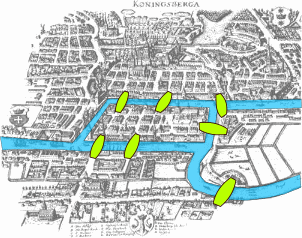
\includegraphics[width=0.7\linewidth]{images/Konigsberg_bridges.png}
\caption{The city of Konigsburg in Euler's time\label{bridges_konigsberg}}
\end{figure}
\hypertarget{p-116}{}%
A group of friends enjoyed strolling through the city, and created a game: could they take a walk in the city, crossing every bridge exactly once, and return to where they started from? They couldn't find such a walk, but they couldn't prove such a walk wasn't possible, and so they wrote to the mathematician Euler, who proved that such a walk is not possible.%
\typeout{************************************************}
\typeout{Subsection 2.2.2 Eulerian Walks: definitions}
\typeout{************************************************}
\subsection[{Eulerian Walks: definitions}]{Eulerian Walks: definitions}\label{subsection-17}
\hypertarget{p-117}{}%
We will formalize the problem presented by the citizens of Konigsburg in graph theory, which will immediately present an obvious generalization.%
\par
\hypertarget{p-118}{}%
We may represent the city of Konigsburg as a graph \(\Gamma_K\); the four sectors of town will be the vertices of \(\Gamma_K\), and edges between vertices will represent the bridges (hence, this will not be a simple graph).%
\par
\hypertarget{p-119}{}%
Then, the question reduces to finding a closed walk in the graph that will uses every edge \emph{exactly} once. In particular, this walk will not use any edge more than once and hence will be a trail.%
\begin{exercise}\label{exercise-8}
\end{exercise}
\begin{definition}[{}]\label{definition-16}
\hypertarget{p-120}{}%
Let \(G\) be a graph.  An \emph{Eulerian cycle} is a closed walk that uses every edge of \(G\) exactly once.%
\par
\hypertarget{p-121}{}%
If \(G\) has an Eulerian cycle, we say that \(G\) is \emph{Eulerian}.%
\par
\hypertarget{p-122}{}%
If we weaken the requirement, and do not require the walk to be closed, we call it an Euler path, and if a graph \(G\) has an Eulerian path but not an Eulerian cycle, we say \(G\) is \emph{semi-Eulerian}%
\end{definition}
\hypertarget{p-123}{}%
The question of the walkers of Konigsburg is then equivalent to asking if the graph \(\Gamma_K\) is Eulerian. The birth of graph theory is usually marked to the following theorem, proven by Euler:%
\begin{theorem}[{}]\label{thm_eulerian}
\hypertarget{p-124}{}%
A connected graph \(\Gamma\) is Eulerian if and only if every vertex of \(\Gamma\) has even degree%
\end{theorem}
\typeout{************************************************}
\typeout{Subsection 2.2.3 A digression on proofs, formality, and intuition}
\typeout{************************************************}
\subsection[{A digression on proofs, formality, and intuition}]{A digression on proofs, formality, and intuition}\label{subsection-18}
\hypertarget{p-125}{}%
Before discussing the proof of \hyperref[thm_eulerian]{Theorem~\ref{thm_eulerian}}, it's worth a little meta-discussion about proofs, intuition vs. rigor, and mathematics as a whole.  The proofing \hyperref[thm_eulerian]{Theorem~\ref{thm_eulerian}} is a common exam question, and you may not be used to studying for reproducing proofs on exams.  Certainly one way to prepare for such a question is to memorize the proof word for word.  There doesn't seem to be a lot of obvious value in this approach, however.  So why ask these questions on the exam? And this opens the door to more philosophical questions as well: how should we think/interact with proofs anyway?  What's the point of it all?%
\par
\hypertarget{p-126}{}%
Usually in books or in lectures, proofs are only given in slick, elegant, polished formal versions.  There are many reasons for this: there's a certain beauty to it; it's important to write it out formally to make sure it's all correct; there's only so much time in lectures, and brevity is a virtue anyway.  People turn away from long works, and the main point of a proof, after all, is to prove something, and it's easier to check that it's all correct if it's shorter.%
\par
\hypertarget{p-127}{}%
But there's a very real downside to this presentation of proofs as the finished, elegant thing.  Most important to me is that the way mathematics is written formally on the page is very different from how it lives actively in our brains (or my brain, at least).  Nobody (or certainly very few people) comes up with proofs in the elegant short start to finish way that they're written.  Typically, there's a mess of chaotic half ideas that slowly get refined down to the written proof that you see.  But often the mess is the exciting part,%
\par
\hypertarget{p-128}{}%
We sketch a few of the main ideas of the proof in an informal setting now, before giving a complete formal proof.  To learn this proof for the exam, you should have this informal picture in your head, and perhaps a skeleton outline of the main formal points that need to be shown.  You shouldn't try to memorize the formal proof word for word like a poem; instead, practice expanding out from the informal ideas/skeleton proof to the full formal proof on your own a few times.%
\par
\hypertarget{p-129}{}%
It is much easier to see that if a graph \(G\) \emph{is} Eulerian, then every vertex has even degree.  Suppose we wanted to show that a given vertex \(v\) was Eulerian; let us stand at the vertex \(v\) and have a friend trace out the Eulerian cycle.  We'll wait for a while, and then the friend will appear at \(v\) along some edge \(e_1\), and then live along some different edge \(e_2\).  We'll wait some more, and they'll reappear coming from new edge \(e_3\), and then leave again along some edge \(e_4\).%
\par
\hypertarget{p-130}{}%
This will continue until they have arrived or left by every edge that hits \(v\).  But every time they visit \(v\), they must arrive by one edge, and leave by another one, and hence every visit uses up an even number of edges, and so the degree \(d(v)\) of \(v\) must be even.  But there was nothing special about the vertex \(v\), and hence the degree of every vertex must be even.%
\par
\hypertarget{p-131}{}%
To argue the other way is more difficult; before trying to show there's a closed path that uses all the edges, let's just construct \emph{any} closed path.  We pick some vertex \(v_0\) to start at, and just randomly choose an edge out of \(v_0\), to some other vertex \(v_1\), and from there randomly choosing any edge we haven't used yet to another vertex \(v_n\), and so on.%
\par
\hypertarget{p-132}{}%
To construct a closed walk, we'd like to show we eventually have to return to \(v_0\).  We're only working with finite graphs, so our walk can't continue forever; the only possibility we have to rule out is that we reach some vertex \(v_n\) and find that we have already used every vertex incident to \(v_n\).  But as we saw before, the path will pair up the edges incident to each vertex as an arriving edge and a departing edge, and we know the degree of \(v_n\) is even.  If the path has already visited \(v_n k\) times, then we'll have used \(2k\) of the edges incident to it; when we arrive for the \(k+1\)st time we'll use one edge, and in all we'll have used \(2k+1\) edges, an odd number; since the degree of \(v_n\) is even there must be at least one edge we haven't used to exit by.%
\par
\hypertarget{p-133}{}%
You might worry that the argument above suggests we can carry on the walk forever, which we obviously can't do since the graph is finite, but the argument above doesn't work for \(v_0\): when we start the path out at \(v_0\), we haven't had to arrive there, and so the edge we initially leave by is not paired with anything.  Therefore, if \(\Gamma\) has all vertices with even degree, and we walk randomly for as long as we can, we'll always get stuck at our starting vertex.%
\par
\hypertarget{p-134}{}%
Hence, we have shown that if \(\Gamma\) is a graph with all vertices having even degree, there will exist some closed walk in \(\Gamma\), but the walk we created was chosen randomly, and there's no guarantee it will include all the edge of \(\Gamma\) -- in all likelihood, it won't.%
\par
\hypertarget{p-135}{}%
But if we look at the edges we haven't used, they will form a simpler graph. \(\Gamma^\prime\).  There's no reason for \(\Gamma^\prime\) to be connected, but it's not too hard to see that every vertex of \(\Gamma^\prime\) will still have even degree: in \(\Gamma\) every vertex had even degree, and we saw in our first proof that a closed walk that doesn't repeat edges uses up an even number of edges at each vertex, and so we'll have an even number of edges left at each point.  Thus, each connected piece of \(\Gamma^\prime\) satisfies the hypothesis of the problem, and is simpler, so we can try to find a closed walk on each of connected piece of \(\Gamma^\prime\), and then "stitch" the results together to get a walk that uses all the pieces. In the formal proof, this process is best captured using induction, and we'll save the complete description until then, but for now we illustrate the process in an example%
\begin{example}[]\label{example-9}
\(\Gamma\)\begin{figure}
\centering
{
\begin{tikzpicture}
\begin{scope}[every node/.style={circle, thick, draw}]
  \node (a) at (0,0) {$a$};
  \node (b) at (1,0) {$b$};
  \node (c) at (2,0) {$c$};
  \node (d) at (3,0) {$d$};
  \node (e) at (0,1) {$e$};
  \node (f) at (1,1) {$f$};
  \node (g) at (2,1) {$g$};
  \node (h) at (0,2) {$h$};
  \node (i) at (1,2) {$i$};
  \node (j) at (2,2) {$j$};
\end{scope}
\draw (a)--(e)--(h)--(i)--(f)--(e)--(i)--(j)--(g)--(c)--(d)--(g)--(b)--(a);
\end{tikzpicture}
}
\caption{A graph \(\Gamma\)\label{fig_euler_example1}}
\end{figure}
\hypertarget{p-136}{}%
It probably isn't hard to immediately find an Eulerian cycle for \(\Gamma\) just by examination, but to illustrate the algorithm to begin with, we are going to deliberately choose a cycle that doesn't use every edge, as shown in the next figure:%
\begin{figure}
\centering
{
\begin{tikzpicture}[scale=2] 


\begin{tikzpicture}[scale=2]




\begin{scope}[every node/.style={circle, thick, draw}]
  \node (a) at (0,0) {$a$};
  \node (b) at (1,0) {$b$};
  \node (c) at (2,0) {$c$};
  \node (d) at (3,0) {$d$};
  \node (e) at (0,1) {$e$};
  \node (f) at (1,1) {$f$};
  \node (g) at (2,1) {$g$};
  \node (h) at (0,2) {$h$};
  \node (i) at (1,2) {$i$};
  \node (j) at (2,2) {$j$};
\end{scope}

\draw[thin, gray] (a)--(e)--(h)--(i)--(f)--(e)--(i)--(j)--(g)--(c)--(d)--(g)--(b)--(a);

\begin{scope}[every edge/.style={draw=red, very thick}, every node/.style={fill=white, circle}]
\path[->] (a) edge node {1} (e);
\path[->] (e) edge node {2} (i);
\path[->] (i) edge node {3} (j);
\path[->] (j) edge node {4} (g);
\path[->] (g) edge node {5} (b);
\path[->] (b) edge node {6} (a);
\end{scope}
}
\caption{Initializing with a closed walk in \(\Gamma\)\label{fig_euler_example2}}
\end{figure}
\end{example}
\hypertarget{p-137}{}%
This process%
\begin{proof}\hypertarget{proof-4}{}
\end{proof}
\begin{remark}[]\label{remark-1}
\hypertarget{p-138}{}%
Note that it does \emph{not} say: "A graph \(\Gamma\) is Eulerian if and only if it is connected and every vertex has even degree." This statement in quotation marks is false, but for "stupid" reasons.  If \(\Gamma\) is Eulerian, and \(E_n\) is the graph with \(n\) vertices wit no edges, then \(\Gamma\sqcup E_n\) is Eulerian but not connected.  These are the only examples of such graphs.%
\end{remark}
\begin{theorem}[{}]\label{theorem-3}
\hypertarget{p-139}{}%
A connected graph \(\Gamma\) is semi-Eulerian if and only if it has exactly two vertices with odd degree.%
\end{theorem}
\begin{proof}\hypertarget{proof-5}{}
\hypertarget{p-140}{}%
A minor modification of our argument for Eulerian graphs shows that the condition is necessary.  Suppose that \(\Gamma\) is semi-Eulerian, with Eulerian path \(v_0, e_1, v_1,e_2,v_3,\dots,e_n,v_n\).  Then at any vertex other than the starting or ending vertices, we can pair the entering and leaving edges up to get an even number of edges.%
\par
\hypertarget{p-141}{}%
However, at the first vertex \(v_0\) the path cleaves along \(e_1\) the first time but never enters it accordingly, so that \(v_0\) has an odd degree; similarly, at \(v_n\) the path enters one final time along \(e_n\) without leaving, and so \(v_n\) also has an odd degree.%
\par
\hypertarget{p-142}{}%
To see the condition is sufficient we could also modify the argument for the Eulerian case slightly, but it is slicker instead to \emph{reduce} to the Eulerian case.  Suppose that \(\Gamma\) is connected, and that vertices \(v\) and \(w\) have odd degree and all other vertices of \(\Gamma\) have even degree.  Then we can construct a new graph \(\Gamma^\prime\) by adding an extra edge \(e=vw\) to \(\Gamma\).  Then \(\Gamma^\prime\) is connected and every vertex has even degree, and so it has an Eulerian cycle.  Deleting the edge \(e\) that we added from this cycle gives an Eulerian path from \(v\) to \(w\) in \(\Gamma\).%
\end{proof}
\typeout{************************************************}
\typeout{Section 2.3 Hamiltonian cycles}
\typeout{************************************************}
\section[{Hamiltonian cycles}]{Hamiltonian cycles}\label{s_walks_hamiltonian}
\hypertarget{p-143}{}%
We now introduce the concept of Hamiltonian walks. Though on the surface the question seems very similar to determining whether or not a graph is Eulerian, it turns out to be much more difficult.%
\begin{definition}[{}]\label{definition-17}
\hypertarget{p-144}{}%
A graph is \emph{Hamiltonian} if it has a closed walk that uses every vertex exactly once; such a path is called a \emph{Hamiltonian cycle}%
\end{definition}
\hypertarget{p-145}{}%
First, some very basic examples:%
\leavevmode%
\begin{enumerate}
\item\hypertarget{li-31}{}The cycle graph \(C_n\) is Hamiltonian.%
\item\hypertarget{li-32}{}Any graph obtained from \(C_n\) by adding edges is Hamiltonian%
\item\hypertarget{li-33}{}The path graph \(P_n\) is \emph{not} Hamiltonian.%
\end{enumerate}
\begin{figure}
\centering
% group protects changes to lengths, releases boxes (?)
{% begin: group for a single side-by-side
% set panel max height to practical minimum, created in preamble
\setlength{\panelmax}{0pt}
\ifdefined\panelboxAimage\else\newsavebox{\panelboxAimage}\fi%
\begin{lrbox}{\panelboxAimage}
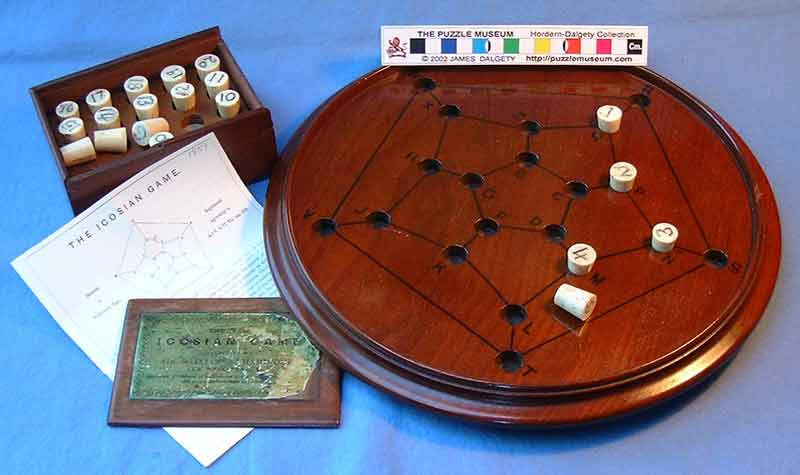
\includegraphics[width=0.4\linewidth]{images/icosiangame.jpg}
\end{lrbox}
\ifdefined\phAimage\else\newlength{\phAimage}\fi%
\setlength{\phAimage}{\ht\panelboxAimage+\dp\panelboxAimage}
\settototalheight{\phAimage}{\usebox{\panelboxAimage}}
\setlength{\panelmax}{\maxof{\panelmax}{\phAimage}}
\ifdefined\panelboxBimage\else\newsavebox{\panelboxBimage}\fi%
\begin{lrbox}{\panelboxBimage}
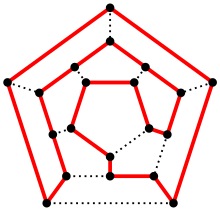
\includegraphics[width=0.4\linewidth]{images/icosiansolved.png}
\end{lrbox}
\ifdefined\phBimage\else\newlength{\phBimage}\fi%
\setlength{\phBimage}{\ht\panelboxBimage+\dp\panelboxBimage}
\settototalheight{\phBimage}{\usebox{\panelboxBimage}}
\setlength{\panelmax}{\maxof{\panelmax}{\phBimage}}
\leavevmode%
% begin: side-by-side as tabular
% \tabcolsep change local to group
\setlength{\tabcolsep}{0.05\linewidth}
% @{} suppress \tabcolsep at extremes, so margins behave as intended
\par\medskip\noindent
\hspace*{0.05\linewidth}%
\begin{tabular}{@{}*{2}{c}@{}}
\begin{minipage}[c][\panelmax][c]{0.4\linewidth}\usebox{\panelboxAimage}\end{minipage}&
\begin{minipage}[c][\panelmax][c]{0.4\linewidth}\usebox{\panelboxBimage}\end{minipage}\end{tabular}\\
% end: side-by-side as tabular
}% end: group for a single side-by-side
\caption{The Icosian game (from \href{https://www.puzzlemuseum.com/month/picm02/200207icosian.htm}{Puzzle Musuem}) and its solution (from \href{https://en.wikipedia.org/wiki/Icosian_game}{Wikipedia})\label{figure-13}}
\end{figure}
\hypertarget{p-146}{}%
The term Hamiltonian comes from William Hamiltonian, who invented (a not very successful) board game he termed the "icosian game", which was about finding Hamiltonian cycles on the dodecahedron graph (and possibly its subgraphs)%
\typeout{************************************************}
\typeout{Exercises 2.4 Exercises}
\typeout{************************************************}
\section[{Exercises}]{Exercises}\label{s_walks_exercises}
\begin{exerciselist}
\item[1.]\hypertarget{exercise-9}{}\hypertarget{p-147}{}%
The questions in this exercise pertain to the graph \(\bfG\) shown in \hyperref[fig_graphs_graph_ex]{Figure~\ref{fig_graphs_graph_ex}}.%
% group protects changes to lengths, releases boxes (?)
{% begin: group for a single side-by-side
% set panel max height to practical minimum, created in preamble
\setlength{\panelmax}{0pt}
\ifdefined\panelboxAol\else\newsavebox{\panelboxAol}\fi%
\savebox{\panelboxAol}{%
\raisebox{\depth}{\parbox{0.6\linewidth}{\leavevmode%
\begin{enumerate}[label=(\alph*)]
\item\hypertarget{li-34}{}\hypertarget{p-148}{}%
What is the degree of vertex \(8\)?%
\item\hypertarget{li-35}{}\hypertarget{p-149}{}%
What is the degree of vertex \(10\)?%
\item\hypertarget{li-36}{}\hypertarget{p-150}{}%
How many vertices of degree \(2\) are there in \(\bfG\)? List them.%
\item\hypertarget{li-37}{}\hypertarget{p-151}{}%
Find a cycle of length \(8\) in \(\bfG\).%
\item\hypertarget{li-38}{}\hypertarget{p-152}{}%
What is the length of a shortest path from \(3\) to \(4\)?%
\item\hypertarget{li-39}{}\hypertarget{p-153}{}%
What is the length of a shortest path from \(8\) to \(7\)?%
\item\hypertarget{li-40}{}\hypertarget{p-154}{}%
Find a path of length \(5\) from vertex \(4\) to vertex \(6\).%
\end{enumerate}
}}}
\ifdefined\phAol\else\newlength{\phAol}\fi%
\setlength{\phAol}{\ht\panelboxAol+\dp\panelboxAol}
\settototalheight{\phAol}{\usebox{\panelboxAol}}
\setlength{\panelmax}{\maxof{\panelmax}{\phAol}}
\ifdefined\panelboxAimage\else\newsavebox{\panelboxAimage}\fi%
\begin{lrbox}{\panelboxAimage}
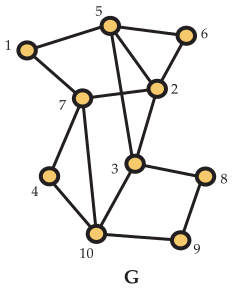
\includegraphics[width=0.35\linewidth]{images/graph_ex}
\end{lrbox}
\ifdefined\phAimage\else\newlength{\phAimage}\fi%
\setlength{\phAimage}{\ht\panelboxAimage+\dp\panelboxAimage}
\settototalheight{\phAimage}{\usebox{\panelboxAimage}}
\setlength{\panelmax}{\maxof{\panelmax}{\phAimage}}
\leavevmode%
% begin: side-by-side as tabular
% \tabcolsep change local to group
\setlength{\tabcolsep}{0.0125\linewidth}
% @{} suppress \tabcolsep at extremes, so margins behave as intended
\par\medskip\noindent
\hspace*{0.0125\linewidth}%
\begin{tabular}{@{}*{2}{c}@{}}
\begin{minipage}[c][\panelmax][t]{0.6\linewidth}\usebox{\panelboxAol}\end{minipage}&
\begin{minipage}[c][\panelmax][t]{0.35\linewidth}\usebox{\panelboxAimage}\end{minipage}\tabularnewline
&
\parbox[t]{0.35\linewidth}{\captionof{figure}{A graph\label{fig_graphs_graph_ex}}
}\end{tabular}\\
% end: side-by-side as tabular
}% end: group for a single side-by-side
\par\smallskip
\item[2.]\hypertarget{exercise-10}{}\hypertarget{p-155}{}%
Draw a graph with \(8\) vertices, all of odd degree, that does not contain a path of length \(3\) or explain why such a graph does not exist.%
\par\smallskip
\item[3.]\hypertarget{exercise-11}{}\hypertarget{p-156}{}%
Find an eulerian circuit in the graph \(\bfG\) in \hyperref[fig_graphs_euler_exercise]{Figure~\ref{fig_graphs_euler_exercise}} or explain why one does not exist.%
\begin{figure}
\centering
{
\begin{overpic}[width=4in]{images/euler_exercise}
                    \put(6,19.5){\(1\)}
                    \put(64.3,5){\(2\)}
                    \put(43.8,15){\(3\)}
                    \put(60,23.5){\(4\)}
                    \put(26,2){\(5\)}
                    \put(21,32){\(6\)}
                    \put(85,9){7}
                    \put(32.3,26.3){\(8\)}
                    \put(53,-1){\(9\)}
                    \put(42,33){\(10\)}
                    \put(71,26){\(11\)}
                    \put(83,21){\(12\)}
                    \end{overpic}
}
\caption{A graph \(\bfG\)\label{fig_graphs_euler_exercise}}
\end{figure}
\par\smallskip
\item[4.]\hypertarget{exercise-12}{}\hypertarget{p-157}{}%
Consider the graph \(\bfG\) in \hyperref[fig_graphs_euler_hamilton_ex]{Figure~\ref{fig_graphs_euler_hamilton_ex}}. Determine if the graph is eulerian. If it is, find an eulerian circuit. If it is not, explain why it is not. Determine if the graph is hamiltonian. If it is, find a hamiltonian cycle. If it is not, explain why it is not.%
\begin{figure}
\centering
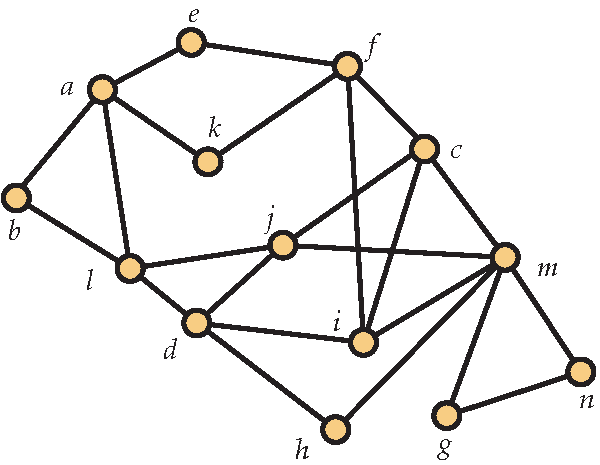
\includegraphics[width=0.65\linewidth]{images/euler_hamilton_ex}
\caption{A graph \(\bfG\)\label{fig_graphs_euler_hamilton_ex}}
\end{figure}
\par\smallskip
\end{exerciselist}
\typeout{************************************************}
\typeout{Chapter 3 Algorithms}
\typeout{************************************************}
\chapter[{Algorithms}]{Algorithms}\label{ch_algorithms}
\hypertarget{p-158}{}%
This chapter covers several graph algorithms.  We start with two algorithms for finding minimal weight spanning trees, Kruskal's algorithm and Prim's algorithm.  We discuss Dijkstra's algorithm for finding the shortest path between two points in a directed, weighted graph.%
\par
\hypertarget{p-159}{}%
Much of the material in this chapter is taken from the open source textbook Applied Combinatorics by Keller and Trotter.%
\typeout{************************************************}
\typeout{Section 3.1 Minimum Weight Spanning Trees}
\typeout{************************************************}
\section[{Minimum Weight Spanning Trees}]{Minimum Weight Spanning Trees}\label{s_graphalgorithms_min-wt-span}
\hypertarget{p-160}{}%
In this section, we consider pairs \((\bfG,w)\) where \(\GVE\) is a connected graph and \(w\colon E\rightarrow\nonnegints\). For each edge \(e\in E\), the quantity \(w(e)\) is called the \terminology{weight}\index{weight} of \(e\). Given a set \(S\) of edges, we define the \terminology{weight} of \(S\), denoted \(w(S)\), by setting \(w(S)=\sum_{e\in S} w(e)\). In particular, the weight of a spanning tree \(T\) is just the sum of the weights of the edges in \(T\).\index{tree!spanning}%
\par
\hypertarget{p-161}{}%
Weighted graphs arise in many contexts. One of the most natural is when the weights on the edges are distances or costs. For example, consider the weighted graph in \hyperref[fig_graphalgorithms_spantreegraph]{Figure~\ref{fig_graphalgorithms_spantreegraph}}. Suppose the vertices represent nodes of a network and the edges represent the ability to establish direct physical connections between those nodes. The weights associated to the edges represent the cost (let's say in thousands of dollars) of building those connections. The company establishing the network among the nodes only cares that there is a way to get data between each pair of nodes. Any additional links would create redundancy in which they are not interested at this time. A spanning tree of the graph ensures that each node can communicate with each of the others and has no redundancy, since removing any edge disconnects it. Thus, to minimize the cost of building the network, we want to find a minimum weight (or cost) spanning tree.%
\begin{figure}
\centering
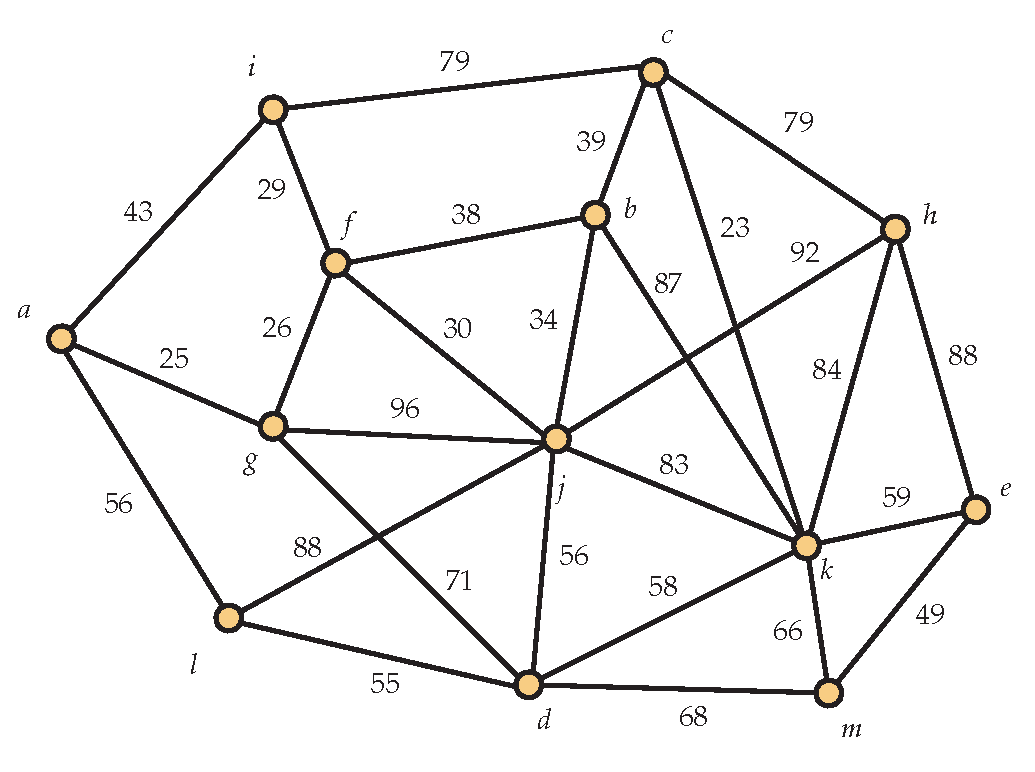
\includegraphics[width=0.9\linewidth]{images/spantreegraph}
\caption{A weighted graph\label{fig_graphalgorithms_spantreegraph}}
\end{figure}
\hypertarget{p-162}{}%
To do this, this section considers the following problem:%
\begin{problem}[]\label{problem-1}
\hypertarget{p-163}{}%
Find a minimum weight spanning tree \(\bfT\) of \(\bfG\).%
\end{problem}
\hypertarget{p-164}{}%
To solve this problem, we will develop \emph{two} efficient graph algorithms, each having certain computational advantages and disadvantages. Before developing the algorithms, we need to establish some preliminaries about spanning trees and forests.%
\typeout{************************************************}
\typeout{Subsection 3.1.1 Preliminaries}
\typeout{************************************************}
\subsection[{Preliminaries}]{Preliminaries}\label{subsection-19}
\hypertarget{p-165}{}%
The following proposition about the number of components in a spanning forest of a graph \(\bfG\) has an easy inductive proof. You are asked to provide it in the exercises.%
\begin{proposition}[{}]\label{prop_graphalgorithms_spanforest}
\hypertarget{p-166}{}%
Let \(\GVE\) be a graph on \(n\) vertices, and let \(\bfH=(V,S)\) be a spanning forest. Then \(0\le |S|\le n-1\). Furthermore, if \(|S|= n-k\), then \(\bfH\) has \(k\) components. In particular, \(\bfH\) is a spanning tree if and only if it contains \(n-1\) edges.%
\end{proposition}
\hypertarget{p-167}{}%
The following proposition establishes a way to take a spanning tree of a graph, remove an edge from it, and add an edge of the graph that is not in the spanning tree to create a new spanning tree. Effectively, the process exchanges two edges to form the new spanning tree, so we call this the \terminology{exchange principle}.%
\begin{proposition}[{Exchange Principle}]\label{prop_graphalgorithms_exchange}
\hypertarget{p-168}{}%
Let \(\bfT=(V,S)\) be spanning tree in a graph \(\bfG\), and let \(e=xy\) be an edge of \(\bfG\) which does not belong to \(\bfT\). Then \leavevmode%
\begin{enumerate}
\item\hypertarget{li-41}{}\hypertarget{p-169}{}%
There is a \emph{unique} path \(P=(x_0,x_1,x_2,\dots,x_t)\) with (a)~\(x=x_0\); (b)~\(y=x_t\); and (c)~\(x_ix_{i+1}\in S\) for each \(i=0,1,2,\dots,t-1\).%
\item\hypertarget{li-42}{}\hypertarget{p-170}{}%
For each \(i=0,1,2,\dots,t-1\), let \(f_i=x_ix_{i+1}\) and then set%
\begin{equation*}
S_i = \{e\}\cup\{g\in S: g\neq f_i\},
\end{equation*}
i.e.\@, we \terminology{exchange} edge \(f_i\) for edge \(e\). Then \(\bfT_i=(V,S_i)\) is a spanning tree of \(\bfG\).%
\end{enumerate}
%
\end{proposition}
\begin{proof}\hypertarget{proof-6}{}
\hypertarget{p-171}{}%
For the first fact, it suffices to note that if there were more than one distinct path from \(x\) to \(y\) in \(\bfT\), we would be able to find a cycle in \(\bfT\). This is impossible since it is a tree. For the second, we refer to \hyperref[fig_graphalgorithms_exchange]{Figure~\ref{fig_graphalgorithms_exchange}}. The black and green edges in the graph shown at the left represent the spanning tree \(\bfT\). Thus, \(f\) lies on the unique path from \(x\) to \(y\) in \(\bfT\) and \(e=xy\) is an edge of \(\bfG\) \emph{not} in \(\bfT\). Adding \(e\) to \(\bfT\) creates a graph with a unique cycle, since \(\bfT\) had a unique path from \(x\) to \(y\). Removing \(f\) (which could be any edge \(f_i\) of the path, as stated in the proposition) destroys this cycle. Thus \(\bfT_i\) is a connected acyclic subgraph of \(\bfG\) with \(n-1+1-1=n-1\) edges, so it is a spanning tree.%
\begin{figure}
\centering
% group protects changes to lengths, releases boxes (?)
{% begin: group for a single side-by-side
% set panel max height to practical minimum, created in preamble
\setlength{\panelmax}{0pt}
\ifdefined\panelboxAimage\else\newsavebox{\panelboxAimage}\fi%
\begin{lrbox}{\panelboxAimage}
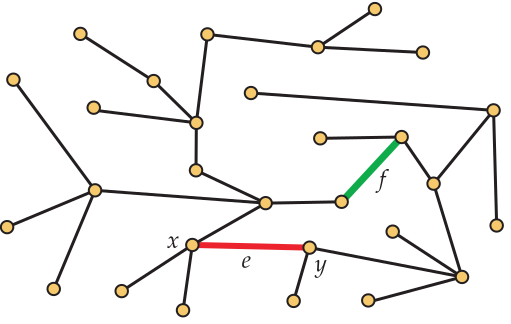
\includegraphics[width=0.48\linewidth]{images/exchange1}
\end{lrbox}
\ifdefined\phAimage\else\newlength{\phAimage}\fi%
\setlength{\phAimage}{\ht\panelboxAimage+\dp\panelboxAimage}
\settototalheight{\phAimage}{\usebox{\panelboxAimage}}
\setlength{\panelmax}{\maxof{\panelmax}{\phAimage}}
\ifdefined\panelboxBimage\else\newsavebox{\panelboxBimage}\fi%
\begin{lrbox}{\panelboxBimage}
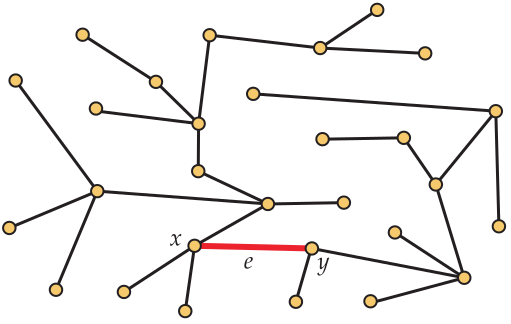
\includegraphics[width=0.48\linewidth]{images/exchange2}
\end{lrbox}
\ifdefined\phBimage\else\newlength{\phBimage}\fi%
\setlength{\phBimage}{\ht\panelboxBimage+\dp\panelboxBimage}
\settototalheight{\phBimage}{\usebox{\panelboxBimage}}
\setlength{\panelmax}{\maxof{\panelmax}{\phBimage}}
\leavevmode%
% begin: side-by-side as tabular
% \tabcolsep change local to group
\setlength{\tabcolsep}{0.01\linewidth}
% @{} suppress \tabcolsep at extremes, so margins behave as intended
\par\medskip\noindent
\hspace*{0.01\linewidth}%
\begin{tabular}{@{}*{2}{c}@{}}
\begin{minipage}[c][\panelmax][t]{0.48\linewidth}\usebox{\panelboxAimage}\end{minipage}&
\begin{minipage}[c][\panelmax][t]{0.48\linewidth}\usebox{\panelboxBimage}\end{minipage}\end{tabular}\\
% end: side-by-side as tabular
}% end: group for a single side-by-side
\caption{The exchange principle\label{fig_graphalgorithms_exchange}}
\end{figure}
\end{proof}
\hypertarget{p-172}{}%
For both of the algorithms we develop, the argument to show that the algorithm is optimal rests on the following technical lemma. To avoid trivialities, we assume \(n\ge3\).%
\begin{lemma}[{}]\label{lem_graphalgorithms_tech}
\hypertarget{p-173}{}%
Let \(\bfF\) be a spanning forest of \(\bfG\) and let \(C\) be a component of \(\bfF\). Also, let \(e=xy\) be an edge of minimum weight among all edges with one endpoint in \(C\) and the other not in \(C\). Then among all spanning trees of \(\bfG\) that contain the forest \(\bfF\), there is one of minimum weight that contains the edge \(e\).%
\end{lemma}
\begin{proof}\hypertarget{proof-7}{}
\hypertarget{p-174}{}%
Let \(\bfT=(V,S)\) be any spanning tree of minimum weight among all spanning trees that contain the forest \(\bfF\), and suppose that \(e=xy\) is not an edge in \(\bfT\). (If it were an edge in \(\bfT\), we would be done.) Then let \(P=(x_0,x_1,x_2,\dots,x_t)\) be the unique path in \(\bfT\) with (a)~\(x=x_0\); (b)~\(y=x_t\); and (c)~\(x_ix_{i+1}\in S\) for each \(i=0,1,2,\dots,t-1\). Without loss of generality, we may assume that \(x=x_0\) is a vertex in \(C\) while \(y=x_t\) does not belong to \(C\). Then there is a least non-negative integer \(i\) for which \(x_i\) is in \(C\) and \(x_{i+1}\) is not in \(C\). It follows that \(x_j\) is in \(C\) for all \(j\) with \(0\le j\le i\).%
\par
\hypertarget{p-175}{}%
Let \(f=x_ix_{i+1}\). The edge \(e\) has minimum weight among all edges with one endpoint in \(C\) and the other not in \(C\), so \(w(e)\le w(f)\). Now let \(\bfT_i\) be the tree obtained by exchanging the edge \(f\) for edge~\(e\). It follows that \(w(\bfT_i) = w(\bfT) - w(f) +w(e)\le w(\bfT)\). Furthermore, \(\bfT_i\) contains the spanning forest \(\bfF\) as well as the edge~\(e\). It is therefore the minimum weight spanning tree we seek.%
\end{proof}
\begin{remark}[]\label{remark-2}
\hypertarget{p-176}{}%
Although Bob's combinatorial intuition has improved over the course he doesn't quite understand why we need special algorithms to find minimum weight spanning trees. He figures there can't be that many spanning trees, so he wants to just write them down. Alice groans as she senses that Bob must have been absent when the material from {$\langle\langle$Unresolved xref, reference "s\_graphs\_counting-trees"; check spelling or use "provisional" attribute$\rangle\rangle$}\hyperlink{}{~} was discussed. In that section, we learned that a graph on \(n\) vertices can have as many as \(n^{n-2}\) spanning trees (or horrors, the instructor may have left it off the syllabus). Regardless, this exhaustive approach is already unusable when \(n = 20\). Dave mumbles something about being greedy and just adding the lightest edges one-by-one while never adding an edge that would make a cycle. Zori remembers a strategy like this working for finding the height of a poset, but she's worried about the nightmare situation that we learned about with using FirstFit to color graphs. Alice agrees that greedy algorithms have an inconsistent track record but suggests that \hyperref[lem_graphalgorithms_tech]{Lemma~\ref{lem_graphalgorithms_tech}} may be enough to get one to succeed here.%
\end{remark}
\typeout{************************************************}
\typeout{Subsection 3.1.2 Kruskal's Algorithm}
\typeout{************************************************}
\subsection[{Kruskal's Algorithm}]{Kruskal's Algorithm}\label{subsection-20}
\hypertarget{p-177}{}%
In this section, we develop one of the best known algorithms for finding a minimum weight spanning tree. It is known as \terminology{Kruskal's Algorithm}, although some prefer the descriptive label \emph{Avoid Cycles} because of the way it builds the spanning tree.%
\par
\hypertarget{p-178}{}%
To start Kruskal's algorithm, we sort the edges according to weight.  To be more precise, let \(m\) denote the number of edges in \(\GVE\).  Then label the edges as \(e_1,e_2,e_3,\dots,e_m\) so that \(w(e_1)\le w(e_2)\le \dots \le w(e_m)\). Any of the many available efficient sorting algorithms can be used to do this step.%
\par
\hypertarget{p-179}{}%
Once the edges are sorted, Kruskal's algorithm proceeds to an initialization step and then inductively builds the spanning tree \(\bfT=(V,S)\):%
\begin{algorithm}[{Kruskal's Algorithm}]\label{alg_kruskal}
\index{minimum weight spanning tree!Kruskal's algorithm for}\index{Kruskal's algorithm}\hypertarget{p-180}{}%
\leavevmode%
\begin{description}
\item[{Initialization.}]\hypertarget{li-43}{}\hypertarget{p-181}{}%
Set \(S=\emptyset\) and \(i=0\).%
\item[{Inductive Step.}]\hypertarget{li-44}{}\hypertarget{p-182}{}%
While \(|S| \lt n-1\), let \(j\) be the least non-negative integer so that \(j > i\) and there are no cycles in \(S\cup\{e_j\}\). Then (using pseudo-code) set%
\begin{equation*}
i = j\quad\text{and} \quad S= S\cup\{j\}.
\end{equation*}
%
\end{description}
%
\end{algorithm}
\hypertarget{p-183}{}%
The correctness of Kruskal's Algorithm follows from an inductive argument. First, the set \(S\) is initialized as the empty set, so there is certainly a minimum weight spanning tree containing all the edges in \(S\). Now suppose that for some \(i\) with \(0\le i \lt n\), \(|S|=i\) and there is a minimum weight spanning tree containing all the edges in \(S\). Let \(\bfF\) be the spanning forest determined by the edges in \(S\), and let \(C_1, C_2,\dots,C_s\) be the components of \(\bfF\). For each \(k=1,2,\dots,s\), let \(f_k\) be a minimum weight edge with one endpoint in \(C_k\) and the other not in \(C_k\). Then the edge \(e\) added to \(S\) by Kruskal's Algorithm is just the edge \(\{f_1,f_2,\dots,f_s\}\) having minimum weight. Applying \hyperref[lem_graphalgorithms_tech]{Lemma~\ref{lem_graphalgorithms_tech}} and the inductive hypothesis, we know that there will still be a minimum weight spanning tree of \(\bfG\) containing all the edges of \(S\cup\{e\}\).%
\begin{example}[Kruskal's Algorithm]\label{example-10}
% group protects changes to lengths, releases boxes (?)
{% begin: group for a single side-by-side
% set panel max height to practical minimum, created in preamble
\setlength{\panelmax}{0pt}
\ifdefined\panelboxAp\else\newsavebox{\panelboxAp}\fi%
\savebox{\panelboxAp}{%
\raisebox{\depth}{\parbox{0.78\linewidth}{Let's see what Kruskal's algorithm does on the weighted graph in \hyperref[fig_graphalgorithms_spantreegraph]{Figure~\ref{fig_graphalgorithms_spantreegraph}}.  It first sorts all of the edges by weight. We won't reproduce the list here, since we won't need all of it. The edge of least weight is \(ck\), which has weight \(23\). It continues adding the edge of least weight, adding \(ag\), \(fg\), \(fi\), \(fj\), and \(bj\). However, after doing this, the edge of lowest weight is \(fb\), which has weight \(38\). This edge cannot be added, as doing so would make \(fjb\) a cycle. Thus, the algorithm bypasses it and adds \(bc\). Edge \(ai\) is next inspected, but it, too, would create a cycle and is eliminated from consideration. Then \(em\) is added, followed by \(dl\). There are now \emph{two} edges of weight \(56\) to be considered: \(al\) and \(dj\). Our sorting algorithm has somehow decided one of them should appear first, so let's say it's \(dj\). After adding \(dj\), we cannot add \(al\), as \(agfjdl\) would form a cycle. Edge \(dk\) is next considered, but it would also form a cycle. However, \(ek\) can be added. Edges \(km\) and \(dm\) are then bypassed. Finally, edge \(ch\) is added as the twelfth and final edge for this \(13\)-vertex spanning tree. The full list of edges added (in order) is shown to the right. The total weight of this spanning tree is \(504\).}}}
\ifdefined\phAp\else\newlength{\phAp}\fi%
\setlength{\phAp}{\ht\panelboxAp+\dp\panelboxAp}
\settototalheight{\phAp}{\usebox{\panelboxAp}}
\setlength{\panelmax}{\maxof{\panelmax}{\phAp}}
\ifdefined\panelboxApre\else\newsavebox{\panelboxApre}\fi%
\begin{lrbox}{\panelboxApre}
\begin{preformattedbox}[boxwidth=0.17\linewidth]
c k 23
a g 25
f g 26
f i 29
f j 30
b j 34
b c 39
e m 49
d l 55
d j 56
e k 59
c h 79
\end{preformattedbox}
\end{lrbox}
\ifdefined\phApre\else\newlength{\phApre}\fi%
\setlength{\phApre}{\ht\panelboxApre+\dp\panelboxApre}
\settototalheight{\phApre}{\usebox{\panelboxApre}}
\setlength{\panelmax}{\maxof{\panelmax}{\phApre}}
\leavevmode%
% begin: side-by-side as tabular
% \tabcolsep change local to group
\setlength{\tabcolsep}{0.0125\linewidth}
% @{} suppress \tabcolsep at extremes, so margins behave as intended
\par\medskip\noindent
\hspace*{0.0125\linewidth}%
\begin{tabular}{@{}*{2}{c}@{}}
\begin{minipage}[c][\panelmax][t]{0.78\linewidth}\usebox{\panelboxAp}\end{minipage}&
\begin{minipage}[c][\panelmax][t]{0.17\linewidth}\usebox{\panelboxApre}\end{minipage}\end{tabular}\\
% end: side-by-side as tabular
}% end: group for a single side-by-side
\end{example}
\typeout{************************************************}
\typeout{Subsection 3.1.3 Prim's Algorithm}
\typeout{************************************************}
\subsection[{Prim's Algorithm}]{Prim's Algorithm}\label{alg_prim}
\hypertarget{p-185}{}%
We now develop \terminology{Prim's Algorithm} for finding a minimum weight spanning tree. This algorithm is also known by a more descriptive label: \emph{Build Tree}. We begin by choosing a root vertex \(r\). Again, the algorithm proceeds with an initialization step followed by a series of inductive steps.%
\begin{algorithm}[{Prim's Algorithm}]\label{algorithm-2}
\index{minimum weight spanning trees!Prim's algorithm for}\index{Prim's algorithm}\hypertarget{p-186}{}%
\leavevmode%
\begin{description}
\item[{Initialization.}]\hypertarget{li-45}{}\hypertarget{p-187}{}%
Set \(W=\{r\}\) and \(S=\emptyset\).%
\item[{Inductive Step.}]\hypertarget{li-46}{}\hypertarget{p-188}{}%
While \(|W| \lt n\), let \(e\) be an edge of minimum weight among all edges with one endpoint in \(W\) and the other not in \(W\).  If \(e=xy\), \(x\in W\) and \(y\not\in W\), update \(W\) and \(S\) by setting (using pseudo-code)%
\begin{equation*}
W = W\cup\{y\}\quad\text{and} \quad S = S\cup\{e\}.
\end{equation*}
%
\end{description}
%
\end{algorithm}
\hypertarget{p-189}{}%
The correctness of Prim's algorithm follows immediately from \hyperref[lem_graphalgorithms_tech]{Lemma~\ref{lem_graphalgorithms_tech}}.%
\begin{example}[Prim's Algorithm]\label{example-11}
% group protects changes to lengths, releases boxes (?)
{% begin: group for a single side-by-side
% set panel max height to practical minimum, created in preamble
\setlength{\panelmax}{0pt}
\ifdefined\panelboxAp\else\newsavebox{\panelboxAp}\fi%
\savebox{\panelboxAp}{%
\raisebox{\depth}{\parbox{0.78\linewidth}{Let's see what Prim's algorithm does on the weighted graph in \hyperref[fig_graphalgorithms_spantreegraph]{Figure~\ref{fig_graphalgorithms_spantreegraph}}. We start with vertex \(a\) as the root vertex. The lightest edge connecting \(a\) (the only vertex in the tree so far) to the rest of the graph is \(ag\). Next, \(fg\) is added. This is followed by \(fi\), \(fj\), \(bj\), and \(bc\). Next, the algorithm identifies \(ck\) as the lightest edge connecting \(\{a,g,i,f,j,b,c\}\) to the remaining vertices. Notice that this is considerably later than Kruskal's algorithm finds the same edge. The algorithm then determines that \(al\) and \(jd\), both of weight \(56\) are the lightest edges connecting vertices in the tree to the other vertices. It picks arbitrarily, so let's say it takes \(al\). It next finds \(dl\), then \(ek\), and then \(em\). The final edge added is \(ch\). The full list of edges added (in order) is shown to the right. The total weight of this spanning tree is \(504\). This (not surprisingly) the same weight we obtained using Kruskal's algorithm. However, notice that the spanning tree found is different, as this one contains \(al\) instead of \(dj\). This is not an issue, of course, since in both cases an arbitrary choice between two edges of equal weight was made.}}}
\ifdefined\phAp\else\newlength{\phAp}\fi%
\setlength{\phAp}{\ht\panelboxAp+\dp\panelboxAp}
\settototalheight{\phAp}{\usebox{\panelboxAp}}
\setlength{\panelmax}{\maxof{\panelmax}{\phAp}}
\ifdefined\panelboxApre\else\newsavebox{\panelboxApre}\fi%
\begin{lrbox}{\panelboxApre}
\begin{preformattedbox}[boxwidth=0.17\linewidth]
a g 25
f g 26
f i 29
f j 30
b j 34
b c 39
c k 23
a l 56
d l 55
e k 59
e m 49
c h 79
\end{preformattedbox}
\end{lrbox}
\ifdefined\phApre\else\newlength{\phApre}\fi%
\setlength{\phApre}{\ht\panelboxApre+\dp\panelboxApre}
\settototalheight{\phApre}{\usebox{\panelboxApre}}
\setlength{\panelmax}{\maxof{\panelmax}{\phApre}}
\leavevmode%
% begin: side-by-side as tabular
% \tabcolsep change local to group
\setlength{\tabcolsep}{0.0125\linewidth}
% @{} suppress \tabcolsep at extremes, so margins behave as intended
\par\medskip\noindent
\hspace*{0.0125\linewidth}%
\begin{tabular}{@{}*{2}{c}@{}}
\begin{minipage}[c][\panelmax][t]{0.78\linewidth}\usebox{\panelboxAp}\end{minipage}&
\begin{minipage}[c][\panelmax][t]{0.17\linewidth}\usebox{\panelboxApre}\end{minipage}\end{tabular}\\
% end: side-by-side as tabular
}% end: group for a single side-by-side
\end{example}
\typeout{************************************************}
\typeout{Subsection 3.1.4 Comments on Efficiency}
\typeout{************************************************}
\subsection[{Comments on Efficiency}]{Comments on Efficiency}\label{subsection-22}
\hypertarget{p-191}{}%
An implementation of Kruskal's algorithm seems to require that the edges be sorted. If the graph has \(n\) vertices and \(m\) edges, this requires \(m\log m\) operations just for the sort. But once the sort is done, the process takes only \(n-1\) steps\textemdash{}provided you keep track of the components as the spanning forest expands.  Regardless, it is easy to see that at most \(O(n^2\log n)\) operations are required.%
\par
\hypertarget{p-192}{}%
On the other hand, an implementation of Prim's algorithm requires the program to conveniently keep track of the edges incident with each vertex and always be able to identify the edge with least weight among subsets of these edges. In computer science, the data structure that enables this task to be carried out is called a \terminology{heap}.%
\typeout{************************************************}
\typeout{Section 3.2 Digraphs}
\typeout{************************************************}
\section[{Digraphs}]{Digraphs}\label{s_graphalgorithms_digraphs}
\hypertarget{p-193}{}%
In this section, we introduce another useful variant of a graph. In a graph, the existence of an edge \(xy\) can be used to model a connection between \(x\) and \(y\) that goes in both ways. However, sometimes such a model is insufficient. For instance, perhaps it is possible to fly from Atlanta directly to Fargo but not possible to fly from Fargo directly to Atlanta. In a graph representing the airline network, an edge between Atlanta and Fargo would lose the information that the flights only operate in one direction. To deal with this problem, we introduce a new discrete structure. A \terminology{digraph}\index{digraph}\index{graph!directed|see{digraph}} \(\bfG\) is a pair \((V,E)\) where \(V\) is a vertex set and \(E\subset V\times V\) with \(x\neq y\) for every \((x,y)\in E\). We consider the pair \((x,y)\) as a \terminology{directed edge}\index{edge!directed} from \(x\) to \(y\). Note that for distinct vertices \(x\) and \(y\) from \(V\), the ordered pairs \((x,y)\) and \((y,x)\) are distinct, so the digraph may have one, both or neither of the directed edges \((x,y)\) and \((y,x)\). This is in contrast to graphs, where edges are sets, so \(\{x,y\}\) and \(\{y,x\}\) are the same.%
\par
\hypertarget{p-194}{}%
Diagrams of digraphs use arrowheads on the edges to indicate direction.  This is illustrated in \hyperref[fig_graphalgorithms_digraph]{Figure~\ref{fig_graphalgorithms_digraph}}. For example, the digraph illustrated there contains the edge \((a,f)\) but not the edge \((f,a)\). It does contain both edges \((c,d)\) and \((d,c)\), however.%
\begin{figure}
\centering
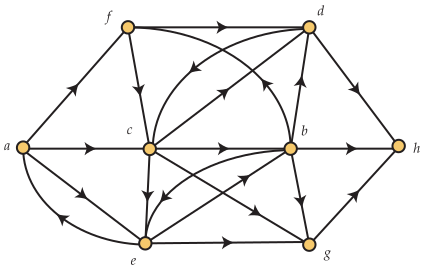
\includegraphics[width=0.85\linewidth]{images/digraph}
\caption{A Digraph\label{fig_graphalgorithms_digraph}}
\end{figure}
\hypertarget{p-195}{}%
When \(\bfG\) is a digraph, a sequence \(P=(r=u_0,u_1,\dots,u_t=x)\) of distinct vertices is called a \terminology{directed path}\index{path!directed} from \(r\) to \(x\) when \((u_iu_{i+1})\) is a directed edge in \(\bfG\) for every \(i=0,1,\dots,t-1\). A directed path \(C=(r=u_0,u_1,\dots,u_t=x)\) is called a \terminology{directed cycle}\index{cycle!directed} when \((u_t,u_0)\) is a directed edge of \(\bfG\).%
\typeout{************************************************}
\typeout{Section 3.3 Dijkstra's Algorithm for Shortest Paths}
\typeout{************************************************}
\section[{Dijkstra's Algorithm for Shortest Paths}]{Dijkstra's Algorithm for Shortest Paths}\label{s_graphalgorithms_shortest-paths}
\hypertarget{p-196}{}%
Just as with graphs, it is useful to assign weights to the directed edges of a digraph. Specifically, in this section we consider a pair \((\bfG,w)\) where \(\GVE\) is a digraph and \(w\colon E\rightarrow\nonnegints\) is a function assigning to each directed edge \((x,y)\) a non-negative weight \(w(x,y)\). However, in this section, we interpret weight as \terminology{distance}\index{distance} so that \(w(x,y)\) is now called the \terminology{length}\index{length} of the edge \((x,y)\). If \(P=(r=u_0,u_1,\dots,u_t=x)\) is a directed path from \(r\) to \(x\), then the \terminology{length} of the path \(P\) is just the sum of the lengths of the edges in the path, \(\sum_{i=0}^{t-1} w(u_iu_{i+1})\). The \terminology{distance} from \(r\) to \(x\) is then defined to be the minimum length of a directed path from \(r\) to \(x\). Our goal in this section is to solve the following natural problem, which has many applications:%
\begin{problem}[]\label{problem-2}
\hypertarget{p-197}{}%
For each vertex \(x\), find the distance from \(r\) to \(x\). Also, find a shortest path from \(r\) to \(x\).%
\end{problem}
\typeout{************************************************}
\typeout{Subsection 3.3.1 Description of the Algorithm}
\typeout{************************************************}
\subsection[{Description of the Algorithm}]{Description of the Algorithm}\label{subsection-23}
\hypertarget{p-198}{}%
To describe \terminology{Dijkstra's algorithm} in a compact manner, it is useful to extend the definition of the function \(w\). We do this by setting \(w(x,y)=\infty\) when \(x\neq y\) and \((x,y)\) is not a directed edge of \(\bfG\). In this way, we will treat \(\infty\) as if it were a number (although it is not!).\footnote{This is not an issue for computer implementation of the algorithm, as instead of using \(\infty\), a value given by the product of the number of vertices and the maximum edge weight may be used to simulate infinity.\label{fn-1}}%
\par
\hypertarget{p-199}{}%
We are now prepared to describe Dijkstra's Algorithm.%
\begin{algorithm}[{Dijkstra's Algorithm}]\label{alg_dijkstra}
\index{Dijkstra's algorithm}\index{graph!shortest path in}\hypertarget{p-200}{}%
Let \(n=|V|\). At Step~\(i\), where \(1\le i\le n\), we will have determined: \leavevmode%
\begin{enumerate}
\item\hypertarget{li-47}{}\hypertarget{p-201}{}%
A sequence \(\sigma=(v_1,v_2,v_3,\dots,v_i)\) of distinct vertices from \(\bfG\) with \(r=v_1\).  These vertices are called \terminology{permanent vertices}, while the remaining vertices will be called \terminology{temporary vertices}.%
\item\hypertarget{li-48}{}\hypertarget{p-202}{}%
For each vertex \(x\in V\), we will have determined a number \(\delta(x)\) and a path \(P(x)\) from \(r\) to \(x\) of length \(\delta(x)\).%
\end{enumerate}
 \leavevmode%
\begin{description}
\item[{Initialization (Step~1)}]\hypertarget{li-49}{}\hypertarget{p-203}{}%
Set \(i=1\). Set \(\delta(r)=0\) and let \(P(r)=(r)\) be the trivial one-point path. Also, set \(\sigma= (r)\). For each \(x\neq r\), set \(\delta(x)= w(r,x)\) and \(P(x)=(r,x)\). Let \(x\) be a temporary vertex for which \(\delta(x)\) is minimum. Set \(v_2 = x\), and update \(\sigma\) by appending \(v_2\) to the end of it. Increment \(i\).%
\item[{Inductive Step (Step~\(i\), \(i>1\))}]\hypertarget{li-50}{}\hypertarget{p-204}{}%
If \(i\lt n\), then for each temporary \(x\), let%
\begin{equation*}
\delta(x) = \min\{\delta(x), \delta(v_i)+w(v_i,x)\}.
\end{equation*}
If this assignment results in a reduction in the value of \(\delta(x)\), let \(P(x)\) be the path obtained by adding \(x\) to the end of \(P(v_i)\).%
\par
\hypertarget{p-205}{}%
Let \(x\) be a temporary vertex for which \(\delta(x)\) is minimum. Set \(v_{i+1}=x\), and update \(\sigma\) by appending \(v_{i+1}\) to it. Increment \(i\).%
\end{description}
%
\end{algorithm}
\typeout{************************************************}
\typeout{Subsection 3.3.2 Example of Dijkstra's Algorithm}
\typeout{************************************************}
\subsection[{Example of Dijkstra's Algorithm}]{Example of Dijkstra's Algorithm}\label{subsection-24}
\hypertarget{p-206}{}%
Before establishing why Dijkstra's algorithm works, it may be helpful to see an example of how it works. To do this, consider the digraph \(\bfG\) shown in \hyperref[fig_graphalgorithms_dijkstragraph]{Figure~\ref{fig_graphalgorithms_dijkstragraph}}. For visual clarity, we have chosen a digraph which is an \terminology{oriented graph}, i.e.\@, for each distinct pair \(x,y\) of vertices, the graph contains at most one of the two possible directed edges \((x,y)\) and \((y,x)\).%
\begin{figure}
\centering
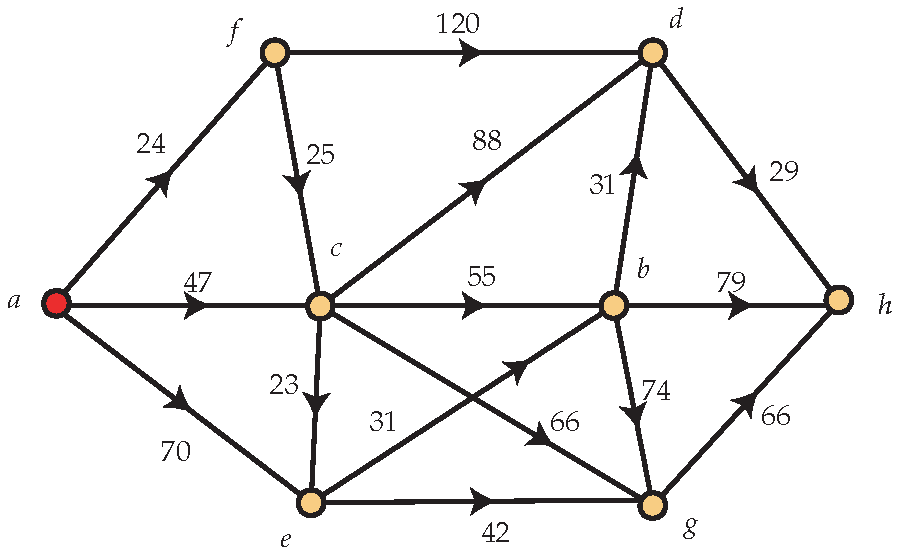
\includegraphics[width=0.85\linewidth]{images/dijkstragraph}
\caption{A digraph with edge lengths\label{fig_graphalgorithms_dijkstragraph}}
\end{figure}
\hypertarget{p-207}{}%
Suppose that the root vertex \(r\) is the vertex labeled~\(a\). The initialization step of Dijkstra's algorithm then results in the following values for \(\delta\) and \(P\):%
\typeout{************************************************}
\typeout{Paragraphs  Step 1. Initialization}
\typeout{************************************************}
\paragraph[{Step 1. Initialization}]{Step 1. Initialization}\hypertarget{paragraphs-1}{}
\hypertarget{p-208}{}%
%
\begin{align*}
\sigma\amp=(a)\amp\amp\\
\delta(a)\amp=0; \amp P(a)\amp=(a)\\
\delta(b) \amp=\infty; \amp P(b)\amp=(a,b)\\
\delta(c) \amp=47; \amp P(c)\amp=(a,c)\\
\delta(d) \amp=\infty; \amp P(d)\amp=(a,d)\\
\delta(e) \amp=70; \amp P(e)\amp=(a,e)\\
\delta(f) \amp=24; \amp P(f)\amp=(a,f)\\
\delta(g) \amp=\infty; \amp P(g)\amp=(a,g)\\
\delta(h) \amp=\infty; \amp P(h)\amp=(a,h)
\end{align*}
%
\par
\hypertarget{p-209}{}%
Before finishing Step 1, the algorithm identifies vertex~\(f\) as closest to \(a\) and appends it to \(\sigma\), making \(a\) permanent. When entering Step 2, Dijkstra's algorithm attempts to find shorter paths from \(a\) to each of the temporary vertices by going through \(f\). We call this process ``scanning from vertex~\(f\).'' In this scan, the path to vertex~\(d\) is updated, since \(\delta(f) + w(f,d)=24+120=144\lt \infty=w(a,d)\).%
\typeout{************************************************}
\typeout{Paragraphs  Step 2.  Scan from vertex~\(f\)}
\typeout{************************************************}
\paragraph[{Step 2.  Scan from vertex~\(f\)}]{Step 2.  Scan from vertex~\(f\)}\hypertarget{paragraphs-2}{}
\hypertarget{p-210}{}%
%
\begin{align*}
\sigma\amp=(a,f)\amp\amp\\
\delta(a)\amp=0; \amp P(a)\amp=(a)\\
\delta(b)\amp=\infty; \amp P(b)\amp=(a,b)\\
\delta(c)\amp=47; \amp P(c)\amp=(a,c)\\
\delta(d)\amp=144 = 24 + 120 = \delta(f)+w(f,d); \amp P(d)\amp=(a,f,d)\quad\text{updated} \\
\delta(e)\amp=70; \amp P(e)\amp=(a,e)\\
\delta(f)\amp=24; \amp P(f)\amp=(a,f)\\
\delta(g)\amp=\infty; \amp P(g)\amp=(a,f)\\
\delta(h)\amp=\infty; \amp P(h)\amp=(a,h)
\end{align*}
%
\par
\hypertarget{p-211}{}%
Before proceeding to the next step, vertex~\(c\) is made permanent by making it \(v_3\). In Step 3, therefore, the scan is from vertex \(c\). Vertices \(b\), \(d\), and \(g\) have their paths updated. However, although \(\delta(c) + w(c,e) = 47+23=70=\delta(e)\), we do not change \(P(e)\) since \(\delta(e)\) is not \emph{decreased} by routing \(P(e)\) through \(c\).%
\typeout{************************************************}
\typeout{Paragraphs  Step 3.  Scan from vertex~\(c\)}
\typeout{************************************************}
\paragraph[{Step 3.  Scan from vertex~\(c\)}]{Step 3.  Scan from vertex~\(c\)}\hypertarget{paragraphs-3}{}
\hypertarget{p-212}{}%
%
\begin{align*}
\sigma\amp=(a,f,c)\\
\delta(a)\amp=0; \amp P(a)\amp=(a)\\
\delta(b)\amp=102=47+55= \delta(c)+w(c,b); \amp P(b)\amp=(a,c,b)\quad\text{updated}\\
\delta(c)\amp=47; \amp P(c)\amp=(a,c)\\
\delta(d)\amp=135=47+88 = \delta(c)+w(c,d); \amp P(d)\amp=(a,c,d)\quad\text{updated} \\
\delta(e)\amp=70; \amp P(e)\amp=(a,e)\\
\delta(f)\amp=24; \amp P(f)\amp=(a,f)\\
\delta(g)\amp=113=47+66= \delta(c)+w(c,g); \amp P(g)\amp=(a,c,g)\quad\text{updated} \\
\delta(h)\amp=\infty; \amp P(h)\amp=(a,h)
\end{align*}
%
\par
\hypertarget{p-213}{}%
Now vertex \(e\) is made permanent.%
\typeout{************************************************}
\typeout{Paragraphs  Step 4.  Scan from vertex~\(e\)}
\typeout{************************************************}
\paragraph[{Step 4.  Scan from vertex~\(e\)}]{Step 4.  Scan from vertex~\(e\)}\hypertarget{paragraphs-4}{}
\hypertarget{p-214}{}%
%
\begin{align*}
\sigma\amp=(a,f,c,e)\\
\delta(a)\amp=0; \amp P(a)\amp=(a)\\
\delta(b)\amp=101=70+31= \delta(e)+w(e,b); \amp P(b)\amp=(a,e,b)\quad\text{updated}\\
\delta(c)\amp=47; \amp P(c)\amp=(a,c)\\
\delta(d)\amp=135; \amp P(d)\amp=(a,c,d)\\
\delta(e)\amp=70; \amp P(e)\amp=(a,e)\\
\delta(f)\amp=24; \amp P(f)\amp=(a,f)\\
\delta(g)\amp=112=70+42= \delta(e)+w(e,g); \amp P(g)\amp=(a,e,g)\quad\text{updated}\\
\delta(h)\amp=\infty; \amp P(h)\amp=(a,h)
\end{align*}
%
\par
\hypertarget{p-215}{}%
Now vertex \(b\) is made permanent.%
\typeout{************************************************}
\typeout{Paragraphs  Step 5.  Scan from vertex~\(b\)}
\typeout{************************************************}
\paragraph[{Step 5.  Scan from vertex~\(b\)}]{Step 5.  Scan from vertex~\(b\)}\hypertarget{paragraphs-5}{}
\hypertarget{p-216}{}%
%
\begin{align*}
\sigma\amp=(a,f,c,e,b)\\
\delta(a)\amp=0; \amp P(a)\amp=(a)\\
\delta(b)\amp=101; \amp P(b)\amp=(a,e,b)\\
\delta(c)\amp=47; \amp P(c)\amp=(a,c)\\
\delta(d)\amp= 132 = 101+ 31= \delta(b)+w(b,d); \amp P(d)\amp=(a,e,b,d)\quad\text{updated} \\
\delta(e)\amp= 70; \amp P(e)\amp=(a,e)\\
\delta(f)\amp= 24; \amp P(f)\amp=(a,f)\\
\delta(g)\amp=112; \amp P(g)\amp=(a,e,g)\\
\delta(h)\amp=180 = 101+79=\delta(b)+w(b,h); \amp P(h)\amp=(a,e,b,h)\quad\text{updated} 
\end{align*}
%
\par
\hypertarget{p-217}{}%
Now vertex \(g\) is made permanent.%
\typeout{************************************************}
\typeout{Paragraphs  Step 6.  Scan from vertex~\(g\)}
\typeout{************************************************}
\paragraph[{Step 6.  Scan from vertex~\(g\)}]{Step 6.  Scan from vertex~\(g\)}\hypertarget{paragraphs-6}{}
\hypertarget{p-218}{}%
%
\begin{align*}
\sigma\amp=(a,f,c,e,b,g)\\
\delta(a)\amp=0; \amp P(a)\amp=(a)\\
\delta(b)\amp=101; \amp P(b)\amp=(a,e,b)\\
\delta(c)\amp=47; \amp P(c)\amp=(a,c)\\
\delta(d)\amp= 132; \amp P(d)\amp=(a,e,b,d)\\
\delta(e)\amp=70; \amp P(e)\amp=(a,e)\\
\delta(f)\amp=24; \amp P(f)\amp=(a,f)\\
\delta(g)\amp=112; \amp P(g)\amp=(a,e,g)\\
\delta(h)\amp=178 = 112+66=\delta(g)+w(g,h); \amp P(h)\amp=(a,e,g,h)\quad\text{updated}
\end{align*}
%
\par
\hypertarget{p-219}{}%
Now vertex \(d\) is made permanent.%
\typeout{************************************************}
\typeout{Paragraphs  Step 7.  Scan from vertex~\(d\)}
\typeout{************************************************}
\paragraph[{Step 7.  Scan from vertex~\(d\)}]{Step 7.  Scan from vertex~\(d\)}\hypertarget{paragraphs-7}{}
\hypertarget{p-220}{}%
%
\begin{align*}
\sigma\amp=(a,f,c,e,b,g,d)\\
\delta(a)\amp=0; \amp P(a)\amp=(a)\\
\delta(b)\amp=101; \amp P(b)\amp=(a,e,b)\\
\delta(c)\amp=47; \amp P(c)\amp=(a,c)\\
\delta(d)\amp= 132; \amp P(d)\amp=(a,e,b,d)\\
\delta(e)\amp=70; \amp P(e)\amp=(a,e)\\
\delta(f)\amp=24; \amp P(f)\amp=(a,f)\\
\delta(g)\amp=112; \amp P(g)\amp=(a,e,g)\\
\delta(h)\amp=161 = 132+29=\delta(d)+w(d,h); \amp P(h)\amp=(a,e,b,d,h)\quad\text{updated}
\end{align*}
%
\par
\hypertarget{p-221}{}%
Now vertex \(h\) is made permanent. Since this is the last vertex, the algorithm halts and returns the following:%
\typeout{************************************************}
\typeout{Paragraphs  Final Results of Dijkstra's Algorithm}
\typeout{************************************************}
\paragraph[{Final Results of Dijkstra's Algorithm}]{Final Results of Dijkstra's Algorithm}\hypertarget{paragraphs-8}{}
\hypertarget{p-222}{}%
%
\begin{align*}
\sigma\amp=(a,f,c,e,b,g,d,h)\\
\delta(a)\amp=0; \amp P(a)\amp=(a)\\
\delta(b)\amp=101; \amp P(b)\amp=(a,e,b)\\
\delta(c)\amp=47; \amp P(c)\amp=(a,c)\\
\delta(d)\amp= 132; \amp P(d)\amp=(a,e,b,d)\\
\delta(e)\amp=70; \amp P(e)\amp=(a,e)\\
\delta(f)\amp=24; \amp P(f)\amp=(a,f)\\
\delta(g)\amp=112; \amp P(g)\amp=(a,e,g)\\
\delta(h)\amp=161; \amp P(h)\amp=(a,e,b,d,h)
\end{align*}
%
\typeout{************************************************}
\typeout{Subsection 3.3.3 The Correctness of Dijkstra's Algorithm}
\typeout{************************************************}
\subsection[{The Correctness of Dijkstra's Algorithm}]{The Correctness of Dijkstra's Algorithm}\label{subsection-25}
\hypertarget{p-223}{}%
Now that we've illustrated Dijkstra's algorithm, it's time to prove that it actually does what we claimed it does: find the distance from the root vertex to each of the other vertices and a path of that length. To do this, we first state two elementary propositions. The first is about shortest paths in general, while the second is specific to the sequence of permanent vertices produced by Dijkstra's algorithm.%
\begin{proposition}[{}]\label{proposition-3}
\hypertarget{p-224}{}%
Let \(x\) be a vertex and let \(P=(r=u_0,u_1,\dots,u_t=x)\) be a shortest path from \(r\) to \(x\). Then for every integer \(j\) with \(0\lt j\lt t\), \((u_0,u_1,\dots,u_j)\) is a shortest path from \(r\) to \(u_j\) and \((u_j,u_{j+1},\dots,u_t)\) is a shortest path from \(u_j\) to \(u_t\)%
\end{proposition}
\begin{proposition}[{}]\label{proposition-4}
\hypertarget{p-225}{}%
When the algorithm halts, let \(\sigma=(v_1,v_2,v_3,\dots,v_n)\).  Then%
\begin{equation*}
\delta(v_1)\le \delta(v_2)\le\dots \le \delta(v_n).
\end{equation*}
%
\end{proposition}
\hypertarget{p-226}{}%
We are now ready to prove the correctness of the algorithm. The proof we give will be inductive, but the induction will have nothing to do with the total number of vertices in the digraph or the step number the algorithm is in.%
\begin{theorem}[{}]\label{theorem-4}
\hypertarget{p-227}{}%
Dijkstra's algorithm yields shortest paths for every vertex \(x\) in \(\bfG\). That is, when Dijkstra's algorithm terminates, for each \(x\in V\), the value \(\delta(x)\) is the distance from \(r\) to \(x\) and \(P(x)\) is a shortest path from \(r\) to \(x\).%
\end{theorem}
\begin{proof}\hypertarget{proof-8}{}
\hypertarget{p-228}{}%
The theorem holds trivially when \(x=r\). So we consider the case where \(x\neq r\). We argue that \(\delta(x)\) is the distance from \(r\) to \(x\) and that \(P(x)\) is a shortest path from \(r\) to \(x\) by induction on the minimum number \(k\) of edges in a shortest path from \(r\) to \(x\). When \(k=1\), the edge \((r,x)\) is a shortest path from \(r\) to \(x\). Since \(v_1=r\), we will set \(\delta(x)=w(r,x)\) and \(P(x)=(r,x)\) at Step~1.%
\par
\hypertarget{p-229}{}%
Now fix a positive integer \(k\). Assume that if the minimum number of edges in a shortest path from \(r\) to \(x\) is at most \(k\), then \(\delta(x)\) is the distance from \(r\) to \(x\) and \(P(x)\) is a shortest path from \(r\) to \(x\). Let \(x\) be a vertex for which the minimum number of edges in a shortest path from \(r\) to \(x\) is \(k+1\). Fix a shortest path \(P=(u_0,u_1,u_2,\dots,u_{k+1})\) from \(r=u_0\) to \(x=u_{k+1}\). Then \(Q=(u_0,u_1,\dots,u_k)\) is a shortest path from \(r\) to \(u_k\). (See \hyperref[fig_graphalgorithms_dijkstra-proof]{Figure~\ref{fig_graphalgorithms_dijkstra-proof}}.)%
\begin{figure}
\centering
{
\begin{overpic}[width=0.6\textwidth]{images/dijkstra-proof}
                        \put(3,13){\(r\)}
                        \put(33,25){\(Q\)}
                        \put(58,3){\(P(u_k)\)}
                        \put(73,28){\(u_k\)}
                        \put(83,25){\(P\)}
                        \put(93,21){\(x\)}
                        \end{overpic}
}
\caption{Shortest paths\label{fig_graphalgorithms_dijkstra-proof}}
\end{figure}
\hypertarget{p-230}{}%
By the inductive hypothesis, \(\delta(u_k)\) is the distance from \(r\) to \(u_k\), and \(P(u_k)\) is a shortest path from \(r\) to \(u_k\). Note that \(P(u_k)\) need not be the same as path \(Q\), as we suggest in \hyperref[fig_graphalgorithms_dijkstra-proof]{Figure~\ref{fig_graphalgorithms_dijkstra-proof}}. However, if distinct, the two paths will have the same length, namely \(\delta(u_k)\).  Also, the distance from \(r\) to \(x\) is \(\delta(u_k)+w(u_k,x)\ge \delta(u_k)\) since \(P\) is a shortest path from \(r\) to \(x\) and \(w(u_k,x)\geq 0\).%
\par
\hypertarget{p-231}{}%
Let \(i\) and \(j\) be the unique integers for which \(u_k=v_i\) and \(x=v_j\). If \(j \lt i\), then%
\begin{equation*}
\delta(x)= \delta(v_j)\le \delta(v_i)= \delta(u_k)\le
\delta(u_k)+w(u_k).
\end{equation*}
Therefore the algorithm has found a path \(P(x)\) from \(r\) to \(x\) having length \(\delta(x)\) which is at most the distance from \(r\) to \(x\). Clearly, this implies that \(\delta(x)\) is the distance from \(r\) to \(x\) and that \(P(x)\) is a shortest path.%
\par
\hypertarget{p-232}{}%
On the other hand, if \(j>i\), then the inductive step at Step~\(i\) results in%
\begin{equation*}
\delta(x)\le \delta(v_i)+w(v_i,y)=\delta(u_k)+w(u_k,x).
\end{equation*}
As before, this implies that \(\delta(x)\) is the distance from \(r\) to \(x\) and that \(P(x)\) is a shortest path.%
\end{proof}
\typeout{************************************************}
\typeout{Section 3.4 Prüfer Codes}
\typeout{************************************************}
\section[{Prüfer Codes}]{Prüfer Codes}\label{s_graphalgorithms_prufer}
\hypertarget{p-233}{}%
This section covers the Prüfer Code, a bijection between labelled trees and certain sequences of integers. This bijection allows us to prove Cayley's theorem, giving a count of such labelled trees.%
\par
\hypertarget{p-234}{}%
Given a combinatorial structure, such as a graph or a tree, it is natural to ask how many of such structures there are.  Often, there is no nice formula, for instance, for the number of different trees on \(n\) vertices there.  But if the vertices are labelled, then it turns out there's a nice answer.%
\begin{definition}[{Labelled tree}]\label{definition-18}
\hypertarget{p-235}{}%
A \emph{labelled tree} on \(n\) vertices is a tree with \(n\) vertices, which are labelled \(1,2,\dots,n.\)%
\end{definition}
\begin{theorem}[{Cayley's Theorem}]\label{theorem-5}
\hypertarget{p-236}{}%
There are \(n^{n-2}\) labelled trees on \(n\) vertices.%
\end{theorem}
\hypertarget{p-237}{}%
One more convenient way of writing down a labelled tree is to write down all the edges.  If there tree has \(n\) vertices, then there are \(n-1\) edges, and writing down all the edges takes \(2n-2\) numbers between \(1...n\).  However, we see that we're writing down the same tree lots of different times, by changing the order of the edges, and which vertex from each edge we write first.  Furthermore, not every sequence of \(2n-2\) numbers between \(1...n\) will result in a tree.%
\par
\hypertarget{p-238}{}%
To fix this problem, we will write down the edges in a particular order.  Every tree has at least two leaves, and deleting a leaf gives a small tree.  We will use these facts to give a systematic ordering to the edges in a labelled tree, as follows: the first edge will be the edge connecting the leaf with the smallest label to the rest of the tree.  We will record that edge, with the leaf on the bottom row, and the "parent" vertex, i.e., the vertex the leaf is connected to, in the top row.  Deleting the leaf and the vertex gives a tree with one fewer vertex, and we iterate the process.%
\begin{algorithm}[{Pruning Algorithm}]\label{algorithm-4}
\hypertarget{p-239}{}%
Input:  A labelled tree \(T\) on \(n\) vertices.%
\par
\hypertarget{p-240}{}%
Output: A \(2\times n-1\) table with entries in \(\{1,\dots,n\}\) that records the edges of \(T\) in a specified order.%
\hypertarget{p-241}{}%
Find the leaf \(v\) with the lowest label; it will have one edge \(e\), connecting it to some vertex (its "parent") \(w\).   Form a new tree \(T^\prime\) by deleting \(v\) and \(e\), and record \(e\) in the output table, putting the deleted vertex \(v\) in the bottom row and its parent \(w\) above it in the top row.%
\end{algorithm}
\hypertarget{p-242}{}%
This method fixes the problem of the ordering of the edges not being unique, but as of now we are still recording more information than needed.  But note the following: since we delete a vertex when we put it in the bottom row, no number will appear twice on the bottom row.  The last column is the last two vertices existing, and if we look at the bottom row and the last entry on the top row, we see that every number from 1 to \(n\) will appear exactly once in these spots.%
\begin{definition}[{Prüfer code}]\label{definition-19}
\hypertarget{p-243}{}%
If record the edges of a tree \(T\) as in the Pruning Algorithm, the first \(n-2\) number appear in the top row is the \emph{Prüfer code of \(T\)}%
\end{definition}
\hypertarget{p-244}{}%
To finish the proof of Cayley's Theorem, we need to show that the Prüfer code is a bijection.  The easiest way to do this is to show that it has an inverse; that is, given any sequence of \(n-2\) numbers between 1 and \(n\), we can construct a tree \(T\) have that sequence as its Prüfer code.%
\par
\hypertarget{p-245}{}%
This is most easily done by filling in the \(n\) numbers we deleted from the table of edges to get the Prüfer code.  We will in the numbers on the bottom row from left to right.  The first number on the bottom row will be the lowest number that does not appear in the Prüfer code.  Delete the first column, and then iterate -- the next number will be the lowest number we haven't used, and that doesn't appear in the remainder of the Prüfer code.%
\par
\hypertarget{p-246}{}%
Another way to phrase the last line, is that the next number filled in is always the lowest number the doesn't appear as the bottom entry on one of the \(n-1\) columns.%
\begin{example}[]\label{example-12}
\hypertarget{p-247}{}%
Suppose \(T\) has Prüfer code 4,4,1,4,5,5. This code has length 6, so we looking to complete it by filling in numbers from 1 to 8. We illustrate the process step by step.%
% group protects changes to lengths, releases boxes (?)
{% begin: group for a single side-by-side
% set panel max height to practical minimum, created in preamble
\setlength{\panelmax}{0pt}
\ifdefined\panelboxAp\else\newsavebox{\panelboxAp}\fi%
\savebox{\panelboxAp}{%
\raisebox{\depth}{\parbox{0.6\linewidth}{The lowest number that doesn't appear is 2, so we fill that in on the bottom of the first column. We no longer have to consider the 4 directly above this 2, as it is not the bottom element of its column.}}}
\ifdefined\phAp\else\newlength{\phAp}\fi%
\setlength{\phAp}{\ht\panelboxAp+\dp\panelboxAp}
\settototalheight{\phAp}{\usebox{\panelboxAp}}
\setlength{\panelmax}{\maxof{\panelmax}{\phAp}}
\ifdefined\panelboxAtabular\else\newsavebox{\panelboxAtabular}\fi%
\savebox{\panelboxAtabular}{%
\raisebox{\depth}{\parbox{0.3\linewidth}{\centering\begin{tabular}{ccccccc}
\multicolumn{1}{cB}{4}&\multicolumn{1}{cB}{4}&\multicolumn{1}{cB}{1}&\multicolumn{1}{cB}{4}&\multicolumn{1}{cB}{5}&\multicolumn{1}{cB}{5}&\tabularnewline\hrulemedium
\multicolumn{1}{cB}{2}&\multicolumn{1}{cB}{}&\multicolumn{1}{cB}{}&\multicolumn{1}{cB}{}&\multicolumn{1}{cB}{}&\multicolumn{1}{cB}{}&
\end{tabular}
}}}
\ifdefined\phAtabular\else\newlength{\phAtabular}\fi%
\setlength{\phAtabular}{\ht\panelboxAtabular+\dp\panelboxAtabular}
\settototalheight{\phAtabular}{\usebox{\panelboxAtabular}}
\setlength{\panelmax}{\maxof{\panelmax}{\phAtabular}}
\leavevmode%
% begin: side-by-side as tabular
% \tabcolsep change local to group
\setlength{\tabcolsep}{0.025\linewidth}
% @{} suppress \tabcolsep at extremes, so margins behave as intended
\par\medskip\noindent
\hspace*{0.025\linewidth}%
\begin{tabular}{@{}*{2}{c}@{}}
\begin{minipage}[c][\panelmax][c]{0.6\linewidth}\usebox{\panelboxAp}\end{minipage}&
\begin{minipage}[c][\panelmax][c]{0.3\linewidth}\usebox{\panelboxAtabular}\end{minipage}\end{tabular}\\
% end: side-by-side as tabular
}% end: group for a single side-by-side
% group protects changes to lengths, releases boxes (?)
{% begin: group for a single side-by-side
% set panel max height to practical minimum, created in preamble
\setlength{\panelmax}{0pt}
\ifdefined\panelboxAp\else\newsavebox{\panelboxAp}\fi%
\savebox{\panelboxAp}{%
\raisebox{\depth}{\parbox{0.6\linewidth}{To fill in the next cell, we put the lowest number not occuring as the lowest element of a column, namely 3.}}}
\ifdefined\phAp\else\newlength{\phAp}\fi%
\setlength{\phAp}{\ht\panelboxAp+\dp\panelboxAp}
\settototalheight{\phAp}{\usebox{\panelboxAp}}
\setlength{\panelmax}{\maxof{\panelmax}{\phAp}}
\ifdefined\panelboxAtabular\else\newsavebox{\panelboxAtabular}\fi%
\savebox{\panelboxAtabular}{%
\raisebox{\depth}{\parbox{0.3\linewidth}{\centering\begin{tabular}{ccccccc}
\multicolumn{1}{cB}{4}&\multicolumn{1}{cB}{4}&\multicolumn{1}{cB}{1}&\multicolumn{1}{cB}{4}&\multicolumn{1}{cB}{5}&\multicolumn{1}{cB}{5}&\tabularnewline\hrulemedium
\multicolumn{1}{cB}{2}&\multicolumn{1}{cB}{3}&\multicolumn{1}{cB}{}&\multicolumn{1}{cB}{}&\multicolumn{1}{cB}{}&\multicolumn{1}{cB}{}&
\end{tabular}
}}}
\ifdefined\phAtabular\else\newlength{\phAtabular}\fi%
\setlength{\phAtabular}{\ht\panelboxAtabular+\dp\panelboxAtabular}
\settototalheight{\phAtabular}{\usebox{\panelboxAtabular}}
\setlength{\panelmax}{\maxof{\panelmax}{\phAtabular}}
\leavevmode%
% begin: side-by-side as tabular
% \tabcolsep change local to group
\setlength{\tabcolsep}{0.025\linewidth}
% @{} suppress \tabcolsep at extremes, so margins behave as intended
\par\medskip\noindent
\hspace*{0.025\linewidth}%
\begin{tabular}{@{}*{2}{c}@{}}
\begin{minipage}[c][\panelmax][c]{0.6\linewidth}\usebox{\panelboxAp}\end{minipage}&
\begin{minipage}[c][\panelmax][c]{0.3\linewidth}\usebox{\panelboxAtabular}\end{minipage}\end{tabular}\\
% end: side-by-side as tabular
}% end: group for a single side-by-side
% group protects changes to lengths, releases boxes (?)
{% begin: group for a single side-by-side
% set panel max height to practical minimum, created in preamble
\setlength{\panelmax}{0pt}
\ifdefined\panelboxAp\else\newsavebox{\panelboxAp}\fi%
\savebox{\panelboxAp}{%
\raisebox{\depth}{\parbox{0.6\linewidth}{And now the lowest term not on the bottom of its column is 6, so we add that:}}}
\ifdefined\phAp\else\newlength{\phAp}\fi%
\setlength{\phAp}{\ht\panelboxAp+\dp\panelboxAp}
\settototalheight{\phAp}{\usebox{\panelboxAp}}
\setlength{\panelmax}{\maxof{\panelmax}{\phAp}}
\ifdefined\panelboxAtabular\else\newsavebox{\panelboxAtabular}\fi%
\savebox{\panelboxAtabular}{%
\raisebox{\depth}{\parbox{0.3\linewidth}{\centering\begin{tabular}{ccccccc}
\multicolumn{1}{cB}{4}&\multicolumn{1}{cB}{4}&\multicolumn{1}{cB}{1}&\multicolumn{1}{cB}{4}&\multicolumn{1}{cB}{5}&\multicolumn{1}{cB}{5}&\tabularnewline\hrulemedium
\multicolumn{1}{cB}{2}&\multicolumn{1}{cB}{3}&\multicolumn{1}{cB}{6}&\multicolumn{1}{cB}{}&\multicolumn{1}{cB}{}&\multicolumn{1}{cB}{}&
\end{tabular}
}}}
\ifdefined\phAtabular\else\newlength{\phAtabular}\fi%
\setlength{\phAtabular}{\ht\panelboxAtabular+\dp\panelboxAtabular}
\settototalheight{\phAtabular}{\usebox{\panelboxAtabular}}
\setlength{\panelmax}{\maxof{\panelmax}{\phAtabular}}
\leavevmode%
% begin: side-by-side as tabular
% \tabcolsep change local to group
\setlength{\tabcolsep}{0.025\linewidth}
% @{} suppress \tabcolsep at extremes, so margins behave as intended
\par\medskip\noindent
\hspace*{0.025\linewidth}%
\begin{tabular}{@{}*{2}{c}@{}}
\begin{minipage}[c][\panelmax][c]{0.6\linewidth}\usebox{\panelboxAp}\end{minipage}&
\begin{minipage}[c][\panelmax][c]{0.3\linewidth}\usebox{\panelboxAtabular}\end{minipage}\end{tabular}\\
% end: side-by-side as tabular
}% end: group for a single side-by-side
% group protects changes to lengths, releases boxes (?)
{% begin: group for a single side-by-side
% set panel max height to practical minimum, created in preamble
\setlength{\panelmax}{0pt}
\ifdefined\panelboxAp\else\newsavebox{\panelboxAp}\fi%
\savebox{\panelboxAp}{%
\raisebox{\depth}{\parbox{0.6\linewidth}{Now the only 1 appearing has an element beneath it, and so 1 gets added in the next column:}}}
\ifdefined\phAp\else\newlength{\phAp}\fi%
\setlength{\phAp}{\ht\panelboxAp+\dp\panelboxAp}
\settototalheight{\phAp}{\usebox{\panelboxAp}}
\setlength{\panelmax}{\maxof{\panelmax}{\phAp}}
\ifdefined\panelboxAtabular\else\newsavebox{\panelboxAtabular}\fi%
\savebox{\panelboxAtabular}{%
\raisebox{\depth}{\parbox{0.3\linewidth}{\centering\begin{tabular}{ccccccc}
\multicolumn{1}{cB}{4}&\multicolumn{1}{cB}{4}&\multicolumn{1}{cB}{1}&\multicolumn{1}{cB}{4}&\multicolumn{1}{cB}{5}&\multicolumn{1}{cB}{5}&\tabularnewline\hrulemedium
\multicolumn{1}{cB}{2}&\multicolumn{1}{cB}{3}&\multicolumn{1}{cB}{6}&\multicolumn{1}{cB}{1}&\multicolumn{1}{cB}{}&\multicolumn{1}{cB}{}&
\end{tabular}
}}}
\ifdefined\phAtabular\else\newlength{\phAtabular}\fi%
\setlength{\phAtabular}{\ht\panelboxAtabular+\dp\panelboxAtabular}
\settototalheight{\phAtabular}{\usebox{\panelboxAtabular}}
\setlength{\panelmax}{\maxof{\panelmax}{\phAtabular}}
\leavevmode%
% begin: side-by-side as tabular
% \tabcolsep change local to group
\setlength{\tabcolsep}{0.025\linewidth}
% @{} suppress \tabcolsep at extremes, so margins behave as intended
\par\medskip\noindent
\hspace*{0.025\linewidth}%
\begin{tabular}{@{}*{2}{c}@{}}
\begin{minipage}[c][\panelmax][c]{0.6\linewidth}\usebox{\panelboxAp}\end{minipage}&
\begin{minipage}[c][\panelmax][c]{0.3\linewidth}\usebox{\panelboxAtabular}\end{minipage}\end{tabular}\\
% end: side-by-side as tabular
}% end: group for a single side-by-side
% group protects changes to lengths, releases boxes (?)
{% begin: group for a single side-by-side
% set panel max height to practical minimum, created in preamble
\setlength{\panelmax}{0pt}
\ifdefined\panelboxAp\else\newsavebox{\panelboxAp}\fi%
\savebox{\panelboxAp}{%
\raisebox{\depth}{\parbox{0.6\linewidth}{And now all the 4s have been passed, so the next number is 4.  We jump ahead and fill in the two numbers under 5 as well:}}}
\ifdefined\phAp\else\newlength{\phAp}\fi%
\setlength{\phAp}{\ht\panelboxAp+\dp\panelboxAp}
\settototalheight{\phAp}{\usebox{\panelboxAp}}
\setlength{\panelmax}{\maxof{\panelmax}{\phAp}}
\ifdefined\panelboxAtabular\else\newsavebox{\panelboxAtabular}\fi%
\savebox{\panelboxAtabular}{%
\raisebox{\depth}{\parbox{0.3\linewidth}{\centering\begin{tabular}{ccccccc}
\multicolumn{1}{cB}{4}&\multicolumn{1}{cB}{4}&\multicolumn{1}{cB}{1}&\multicolumn{1}{cB}{4}&\multicolumn{1}{cB}{5}&\multicolumn{1}{cB}{5}&\tabularnewline\hrulemedium
\multicolumn{1}{cB}{2}&\multicolumn{1}{cB}{3}&\multicolumn{1}{cB}{6}&\multicolumn{1}{cB}{1}&\multicolumn{1}{cB}{4}&\multicolumn{1}{cB}{7}&
\end{tabular}
}}}
\ifdefined\phAtabular\else\newlength{\phAtabular}\fi%
\setlength{\phAtabular}{\ht\panelboxAtabular+\dp\panelboxAtabular}
\settototalheight{\phAtabular}{\usebox{\panelboxAtabular}}
\setlength{\panelmax}{\maxof{\panelmax}{\phAtabular}}
\leavevmode%
% begin: side-by-side as tabular
% \tabcolsep change local to group
\setlength{\tabcolsep}{0.025\linewidth}
% @{} suppress \tabcolsep at extremes, so margins behave as intended
\par\medskip\noindent
\hspace*{0.025\linewidth}%
\begin{tabular}{@{}*{2}{c}@{}}
\begin{minipage}[c][\panelmax][c]{0.6\linewidth}\usebox{\panelboxAp}\end{minipage}&
\begin{minipage}[c][\panelmax][c]{0.3\linewidth}\usebox{\panelboxAtabular}\end{minipage}\end{tabular}\\
% end: side-by-side as tabular
}% end: group for a single side-by-side
% group protects changes to lengths, releases boxes (?)
{% begin: group for a single side-by-side
% set panel max height to practical minimum, created in preamble
\setlength{\panelmax}{0pt}
\ifdefined\panelboxAp\else\newsavebox{\panelboxAp}\fi%
\savebox{\panelboxAp}{%
\raisebox{\depth}{\parbox{0.6\linewidth}{The two numbers we haven't used yet are 5 and 8, so they are the entries in the last column, giving us the completed table of edges}}}
\ifdefined\phAp\else\newlength{\phAp}\fi%
\setlength{\phAp}{\ht\panelboxAp+\dp\panelboxAp}
\settototalheight{\phAp}{\usebox{\panelboxAp}}
\setlength{\panelmax}{\maxof{\panelmax}{\phAp}}
\ifdefined\panelboxAtabular\else\newsavebox{\panelboxAtabular}\fi%
\savebox{\panelboxAtabular}{%
\raisebox{\depth}{\parbox{0.3\linewidth}{\centering\begin{tabular}{ccccccc}
\multicolumn{1}{cB}{4}&\multicolumn{1}{cB}{4}&\multicolumn{1}{cB}{1}&\multicolumn{1}{cB}{4}&\multicolumn{1}{cB}{5}&\multicolumn{1}{cB}{5}&8\tabularnewline\hrulemedium
\multicolumn{1}{cB}{2}&\multicolumn{1}{cB}{3}&\multicolumn{1}{cB}{6}&\multicolumn{1}{cB}{1}&\multicolumn{1}{cB}{4}&\multicolumn{1}{cB}{7}&5
\end{tabular}
}}}
\ifdefined\phAtabular\else\newlength{\phAtabular}\fi%
\setlength{\phAtabular}{\ht\panelboxAtabular+\dp\panelboxAtabular}
\settototalheight{\phAtabular}{\usebox{\panelboxAtabular}}
\setlength{\panelmax}{\maxof{\panelmax}{\phAtabular}}
\leavevmode%
% begin: side-by-side as tabular
% \tabcolsep change local to group
\setlength{\tabcolsep}{0.025\linewidth}
% @{} suppress \tabcolsep at extremes, so margins behave as intended
\par\medskip\noindent
\hspace*{0.025\linewidth}%
\begin{tabular}{@{}*{2}{c}@{}}
\begin{minipage}[c][\panelmax][c]{0.6\linewidth}\usebox{\panelboxAp}\end{minipage}&
\begin{minipage}[c][\panelmax][c]{0.3\linewidth}\usebox{\panelboxAtabular}\end{minipage}\end{tabular}\\
% end: side-by-side as tabular
}% end: group for a single side-by-side
\hypertarget{p-254}{}%
Having constructed the table encoding all the edges, we can now draw the labelled tree with those edges%
\begin{figure}
\centering
{
\begin{tikzpicture} 
\begin{scope}[scale=2, every node/.style={circle, thick, draw}]
    \node (1) at (0,0) {1};
    \node (6) at (0,1) {6};
    \node (4) at (1,0) {4};
    \node (2) at (1,1) {2};
    \node (5) at (2,0) {5};
    \node (3) at (2,1) {3};
    \node (7) at (3,0) {7};
    \node (8) at (3,1) {8};

\draw (6)--(1)--(4)--(5)--(7);
\draw (2)--(4)--(3);
\draw (5)--(8);
\end{scope}
\end{tikzpicture}
}
\caption{The tree with Prüfer code 441455\label{fig_pruferbackexample}}
\end{figure}
\end{example}
\typeout{************************************************}
\typeout{Exercises 3.5 Exercises}
\typeout{************************************************}
\section[{Exercises}]{Exercises}\label{s_graphalgorithms_exercises}
\begin{exerciselist}
\item[1.]\hypertarget{exercise-13}{}\hypertarget{p-255}{}%
For the graph in \hyperref[fig_span_tree_ex1]{Figure~\ref{fig_span_tree_ex1}}, use Kruskal's algorithm (``avoid cycles'') to find a minimum weight spanning tree. Your answer should include a complete list of the edges, indicating which edges you take for your tree and which (if any) you reject in the course of running the algorithm.%
\begin{figure}
\centering
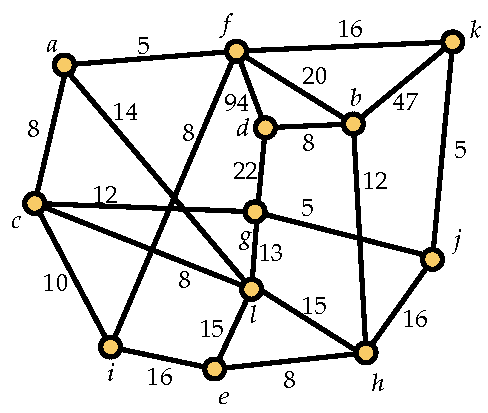
\includegraphics[width=0.65\linewidth]{images/span_tree_ex1}
\caption{Find a minimum weight spanning tree\label{fig_span_tree_ex1}}
\end{figure}
\par\smallskip
\item[2.]\hypertarget{exercise-14}{}\hypertarget{p-256}{}%
For the graph in \hyperref[fig_span_tree_ex1]{Figure~\ref{fig_span_tree_ex1}}, use Prim's algorithm (``build tree'') to find a minimum weight spanning tree. Your answer should list the edges selected by the algorithm in the order they were selected.%
\par\smallskip
\item[3.]\hypertarget{exercise-15}{}\hypertarget{p-257}{}%
For the graph in \hyperref[fig_span_tree_ex2]{Figure~\ref{fig_span_tree_ex2}}, use Kruskal's algorithm (``avoid cycles'') to find a minimum weight spanning tree. Your answer should include a complete list of the edges, indicating which edges you take for your tree and which (if any) you reject in the course of running the algorithm.%
\begin{figure}
\centering
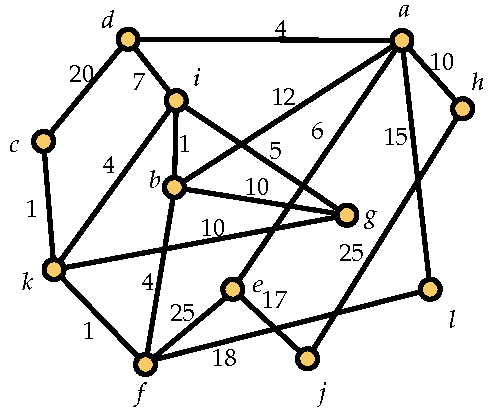
\includegraphics[width=0.65\linewidth]{images/span_tree_ex2}
\caption{Find a minimum weight spanning tree\label{fig_span_tree_ex2}}
\end{figure}
\par\smallskip
\item[4.]\hypertarget{exercise-16}{}\hypertarget{p-258}{}%
For the graph in \hyperref[fig_span_tree_ex2]{Figure~\ref{fig_span_tree_ex2}}, use Prim's algorithm (``build tree'') to find a minimum weight spanning tree. Your answer should list the edges selected by the algorithm in the order they were selected.%
\par\smallskip
\item[5.]\hypertarget{exercise-17}{}\hypertarget{p-259}{}%
For the graph in \hyperref[fig_span_tree_ex3]{Figure~\ref{fig_span_tree_ex3}}, use Kruskal's algorithm (``avoid cycles'') to find a minimum weight spanning tree. Your answer should include a complete list of the edges, indicating which edges you take for your tree and which (if any) you reject in the course of running the algorithm.%
\begin{figure}
\centering
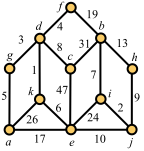
\includegraphics[width=0.45\linewidth]{images/span_tree_ex3}
\caption{Find a minimum weight spanning tree\label{fig_span_tree_ex3}}
\end{figure}
\par\smallskip
\item[6.]\hypertarget{exercise-18}{}\hypertarget{p-260}{}%
For the graph in \hyperref[fig_span_tree_ex3]{Figure~\ref{fig_span_tree_ex3}}, use Prim's algorithm (``build tree'') to find a minimum weight spanning tree. Your answer should list the edges selected by the algorithm in the order they were selected.%
\par\smallskip
\item[7.]\hypertarget{exercise-19}{}\hypertarget{p-261}{}%
A new local bank is being created and will establish a headquarters \(h\), two branches \(b_1\) and \(b_2\), and four ATMs \(a_1\), \(a_2\), \(a_3\), and \(a_4\). They need to build a computer network such that the headquarters, branches, and ATMs can all intercommunicate. Furthermore, they will need to be networked with the Federal Reserve Bank of Atlanta, \(f\). The costs of the feasible network connections (in units of \textdollar{}10,000) are listed below:%
\begin{align*}
h f \amp  \quad 80 \amp 
h b_1 \amp  \quad 10\amp  h b_2 \amp  \quad 20\amp 
b_1 b_2 \amp  \quad 8\\
f b_1 \amp  \quad 12\amp 
f a_1 \amp  \quad 20\amp  b_1 a_1 \amp  \quad 3\amp 
a_1 a_2 \amp  \quad 13\\
h a_2 \amp  \quad 6\amp 
b_2 a_2 \amp  \quad 9\amp  b_2 a_3 \amp  \quad 40\amp 
a_1 a_4 \amp  \quad 3\\
a_3 a_4 \amp \quad 6
\end{align*}
The bank wishes to minimize the cost of building its network (which must allow for connection, possibly routed through other nodes, from each node to each other node), however due to the need for high-speed communication, they \alert{must} pay to build the connection from \(h\) to \(f\) as well as the connection from \(b_2\) to \(a_3\). Give a list of the connections the bank should establish in order to minimize their total cost, subject to this constraint. Be sure to explain how you selected the connections and how you know the total cost is minimized.%
\par\smallskip
\item[8.]\hypertarget{exercise-20}{}\hypertarget{p-262}{}%
A disconnected weighted graph obviously has no spanning trees. However, it is possible to find a spanning forest of minimum weight in such a graph. Explain how to modify both Kruskal's algorithm and Prim's algorithm to do this.%
\par\smallskip
\item[9.]\hypertarget{exercise-21}{}\hypertarget{p-263}{}%
Prove \hyperref[prop_graphalgorithms_spanforest]{Proposition~\ref{prop_graphalgorithms_spanforest}}.%
\par\smallskip
\item[10.]\hypertarget{exercise-22}{}\hypertarget{p-264}{}%
In the paper where Kruskal's algorithm first appeared, he considered the algorithm a route to a nicer proof that in a connected weighted graph with no two edges having the same weight, there is a \emph{unique} minimum weight spanning tree. Prove this fact using Kruskal's algorithm.%
\par\smallskip
\item[11.]\hypertarget{exercise-23}{}\hypertarget{p-265}{}%
Use Dijkstra's algorithm to find the distance from \(a\) to each other vertex in the digraph shown in \hyperref[fig_graphalgorithms_dijkstra_ex1]{Figure~\ref{fig_graphalgorithms_dijkstra_ex1}} and a directed path of that length.%
\begin{figure}
\centering
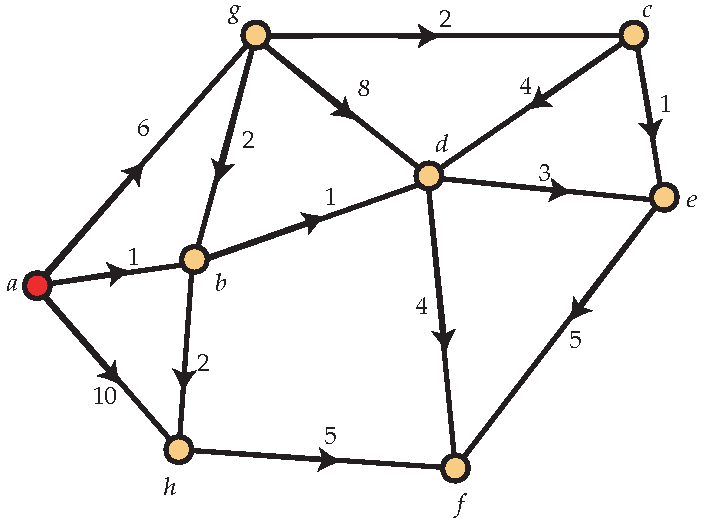
\includegraphics[width=0.65\linewidth]{images/dijkstra_ex1}
\caption{A directed graph\label{fig_graphalgorithms_dijkstra_ex1}}
\end{figure}
\par\smallskip
\item[12.]\hypertarget{exercise-24}{}\hypertarget{p-266}{}%
\hyperref[tab_digraph1]{Table~\ref{tab_digraph1}} contains the length of the directed edge \((x,y)\) in the intersection of \emph{row} \(x\) and \emph{column} \(y\) in a digraph with vertex set \(\{a,b,c,d,e,f\}\). For example, \(w(b,d)=21\). (On the other hand, \(w(d,b)=10\).) Use this data and Dijkstra's algorithm to find the distance from \(a\) to each of the other vertices and a directed path of that length from \(a\).%
\begin{table}
\centering
\begin{tabular}{lAllllll}
\(w\)&\(a\)&\(b\)&\(c\)&\(d\)&\(e\)&\(f\)\tabularnewline\hrulethin
\(a\)&0&12&8&43&79&35\tabularnewline[0pt]
\(b\)&93&0&18&21&60&33\tabularnewline[0pt]
\(c\)&17&3&0&37&50&30\tabularnewline[0pt]
\(d\)&85&10&91&0&17&7\tabularnewline[0pt]
\(e\)&28&47&39&14&0&108\tabularnewline[0pt]
\(f\)&31&7&29&73&20&0
\end{tabular}
\caption{A digraph represented as a table of data\label{tab_digraph1}}
\end{table}
\par\smallskip
\item[13.]\hypertarget{exercise-25}{}\hypertarget{p-267}{}%
Use Dijkstra's algorithm to find the distance from \(a\) to each other vertex in the digraph shown in \hyperref[fig_graphalgorithms_dijkstra_ex2]{Figure~\ref{fig_graphalgorithms_dijkstra_ex2}} and a directed path of that length.%
\begin{figure}
\centering
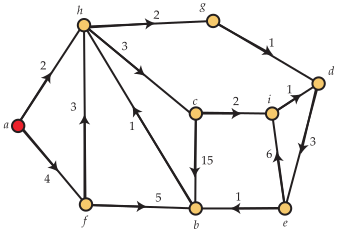
\includegraphics[width=0.65\linewidth]{images/dijkstra_ex2}
\caption{A directed graph\label{fig_graphalgorithms_dijkstra_ex2}}
\end{figure}
\par\smallskip
\item[14.]\hypertarget{exercise-26}{}\hypertarget{p-268}{}%
\hyperref[tab_digraph2]{Table~\ref{tab_digraph2}} contains the length of the directed edge \((x,y)\) in the intersection of \emph{row} \(x\) and \emph{column} \(y\) in a digraph with vertex set \(\{a,b,c,d,e,f\}\). For example, \(w(b,d)=47\). (On the other hand, \(w(d,b)=6\).) Use this data and Dijkstra's algorithm to find the distance from \(a\) to each of the other vertices and a directed path of that length from \(a\).%
\begin{table}
\centering
\begin{tabular}{lAllllll}
\(w\)&\(a\)&\(b\)&\(c\)&\(d\)&\(e\)&\(f\)\tabularnewline\hrulethin
\(a\)&0&7&17&55&83&42\tabularnewline[0pt]
\(b\)&14&0&13&47&27&17\tabularnewline[0pt]
\(c\)&37&42&0&16&93&28\tabularnewline[0pt]
\(d\)&10&6&8&0&4&32\tabularnewline[0pt]
\(e\)&84&19&42&8&0&45\tabularnewline[0pt]
\(f\)&36&3&76&5&17&0
\end{tabular}
\caption{A digraph represented as a table of data\label{tab_digraph2}}
\end{table}
\par\smallskip
\item[15.]\hypertarget{exercise-27}{}\hypertarget{p-269}{}%
Give an example of a digraph having an \emph{undirected} path between each pair of vertices, but having a root vertex \(r\) so that Dijkstra's algorithm cannot find a path of finite length from \(r\) to some vertex \(x\).%
\par\smallskip
\item[16.]\hypertarget{exercise-28}{}\hypertarget{p-270}{}%
Notice that in our discussion of Dijkstra's algorithm, we required that the edge weights be nonnegative. If the edge weights are lengths and meant to model distance, this makes perfect sense. However, in some cases, it might be reasonable to allow negative edge weights. For example, suppose that a positive weight means there is a cost to travel along the directed edge while a negative edge weight means that you make money for traveling along the directed edge. In this case, a directed path with positive total weight results in paying out to travel it, while one with negative total weight results in a profit. \leavevmode%
\begin{enumerate}[label=(\alph*)]
\item\hypertarget{li-51}{}\hypertarget{p-271}{}%
Give an example to show that Dijkstra's algorithm does not always find the path of minimum total weight when negative edge weights are allowed.%
\item\hypertarget{li-52}{}\hypertarget{p-272}{}%
Bob and Xing are considering this situation, and Bob suggests that a little modification to the algorithm should solve the problem. He says that if there are negative weights, they just have to find the smallest (i.e.\@, most negative weight) and add the absolute value of that weight to every directed edge. For example, if \(w(x,y)\geq -10\) for every directed edge \((x,y)\), Bob is suggesting that they add \(10\) to every edge weight. Xing is skeptical, and for good reason. Give an example to show why Bob's modification won't work.%
\end{enumerate}
%
\par\smallskip
\end{exerciselist}
\typeout{************************************************}
\typeout{Chapter 4 Graphs on Surfaces}
\typeout{************************************************}
\chapter[{Graphs on Surfaces}]{Graphs on Surfaces}\label{ch_graphs_on_surfaces}
\hypertarget{p-273}{}%
This chapter covers drawing graphs on surfaces.  We start with discussing whether or not graphs are planar, proving that \(K_{3,3}\) and \(K_5\) are not planar using a method we call the Planarity Algorithm for Hamiltonian graphs.  We discuss the more general Kuratowski's theorem for proving any graph is planar or not.  We introduce other surfaces, and how to draw graphs on them -- the sphere, Mobius band, and torus in particular.  After a brief discussion of dual graphs, we prove Euler's theorem about planar graphs and explore several applications.%
\typeout{************************************************}
\typeout{Section 4.1 Introduction to Graphs on Surfaces: Planarity Algorithm}
\typeout{************************************************}
\section[{Introduction to Graphs on Surfaces: Planarity Algorithm}]{Introduction to Graphs on Surfaces: Planarity Algorithm}\label{s_graphs_on_surfaces_introduction_planarity}
\hypertarget{p-274}{}%
We begin our study of graphs on surfaces with an old chestnut of a problem, the solution of which we will develop into a more general algorithm.%
\typeout{************************************************}
\typeout{Subsection 4.1.1 The Utilities Problem}
\typeout{************************************************}
\subsection[{The Utilities Problem}]{The Utilities Problem}\label{subsection-26}
\hypertarget{p-275}{}%
Suppose there are three houses, owned by Alice, Bob, and Carol, and they'd each like to be connected to one of three Utilities, say, gas, electricity, and water.  There is no real difficulty in the real world, but if we add the restriction that we don't want any of the lines to cross over or under each other, the problem becomes quite interesting.  A failed attempt at drawing a solution is shown here.%
\begin{figure}
\centering
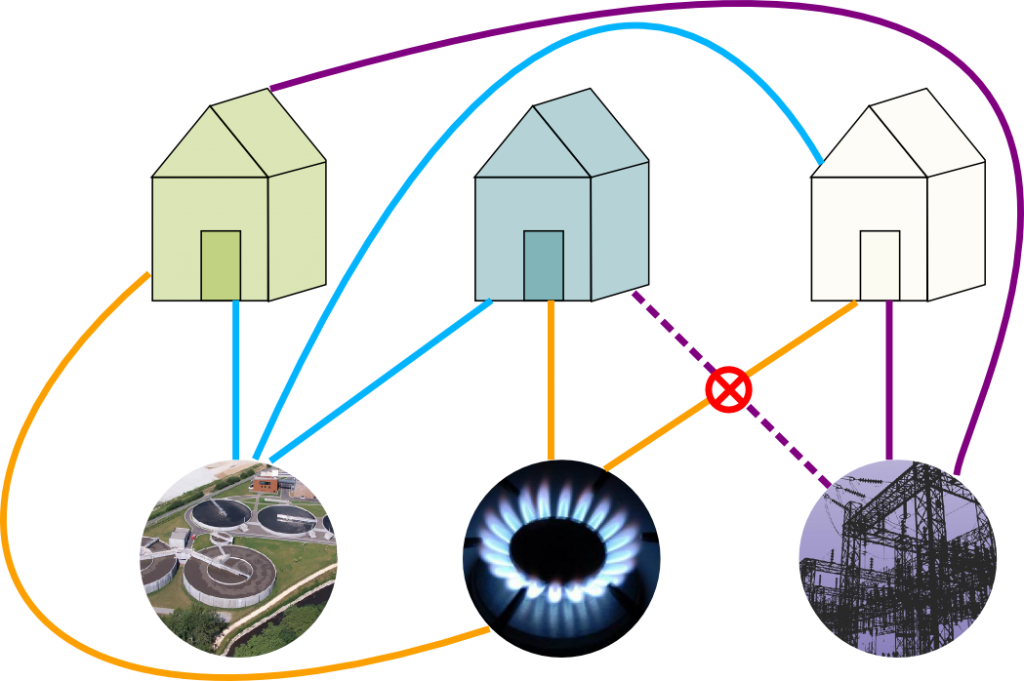
\includegraphics[width=0.7\linewidth]{images/The-Utilities-Problem-Bad-Solution.png}
\caption{An attempt at solving the three utilities problem\label{failed_utilities}}
\end{figure}
\hypertarget{p-276}{}%
Although this attempt failed, it seems very difficult to rule out that some other attempt wouldn't succeed; trying to make a case by case argument seems quite difficult to organize, and it's not clear that there are even finitely many possibilities.  We need a careful way to approach the problem, which we will do in a moment, but first we will use this problem as motivation to make a few definitions.%
\typeout{************************************************}
\typeout{Subsection 4.1.2 }
\typeout{************************************************}
\subsection[{}]{}\label{subsection-27}
\begin{definition}[{}]\label{definition-20}
\hypertarget{p-277}{}%
A graph is \emph{planar} if it can be drawn on a piece of paper so that no edges cross.%
\end{definition}
\hypertarget{p-278}{}%
That definition is a bit loose -- for instance, it's left implicit, we're drawing the edges as lines, with the endpoints being the two vertices it connects.  But this will be strong enough for our purposes.%
\par
\hypertarget{p-279}{}%
With this definition in hand, the Utilities Question is asking whether the graph \(K_{3,3}\) is planar -- treat the three utilities as red vertices, say, and the three houses as the blue vertices.  This doesn't really help us organize our proof, however. To do that, we will use the basic fact that any circle drawn on the plane has an inside and an outside.%
\par
\hypertarget{p-280}{}%
This last fact sounds absolutely trivial, but first, it is not true on other surfaces, for instance, on the torus -- in our video game world, the top of the screen makes a circle, but a point just above this circle is really at the bottom of the video game world, and so the circle doesn't cut the torus into two pieces; I also illustrated this with the Mobius band: the central line down the middle doesn't separate it into two pieces.  This fact is usually stated as follows:%
\begin{theorem}[{Jordan Curve Theorem}]\label{theorem-6}
\hypertarget{p-281}{}%
Any simple closed plane curve has an interior and an exterior%
\end{theorem}
\hypertarget{p-282}{}%
Though easy to state, and intuitively obvious, the Jordan Curve Theorem is surprisingly subtle and difficult to prove; we won't use any more topology than this.%
\par
\hypertarget{p-283}{}%
Before seeing it in practice, let's discuss informally how the Jordan Curve Theorem can be used to help prove whether a graph \(G\) is planar or not.  Suppose that we have found a large cycle \(C_k\) as a subgraph of \(G\).  Then, if we had a planar drawing of \(G\), this cycle would have to appear as a circle.  By the Jordan Curve Theorem, this circle would have an inside and an outside, and every vertex and edge not in our cycle \(C_k\) would have to be either entirely within the circle, or entirely outside the circle.  This gives us a way to organize the case by case argument.%
\par
\hypertarget{p-284}{}%
The bigger a cycle we can find, the fewer other vertices and edges we need to consider, and so we have a much cleaner case by case argument.  In the best cases, the graph is Hamiltonian and the cycle \(C_k\) includes all the vertices of \(G\), and we only have to do a case by case analysis for some the remaining edges.%
\par
\hypertarget{p-285}{}%
Let's see how this general principle gets illustrated in practice%
\begin{theorem}[{}]\label{theorem-7}
\(K_{3,3}\)\end{theorem}
\begin{proof}\hypertarget{proof-9}{}
\hypertarget{p-286}{}%
First let's name the vertices of \(K_{3,3}\): let the vertices \(a,b,c\) be the red and vertices and \(x,y,z\) be the blue vertices.  Then the path \(a-x-b-y-c-z-a\) is a Hamiltonian cycle, and so if \(K_{3,3}\) were planar it would be drawn as a circle in the plane, as shown below:%
\begin{figure}
\centering
{
\begin{tikzpicture}[scale=.7]
\tikzstyle{vertex}=[circle, draw, minimum size=17pt, inner sep=0pt]
\node[vertex, blue] (a) at (0,1) {$a$};
\node[vertex, red] (x) at (1,2) {$x$};
\node[vertex, blue] (b) at (3,2) {$b$};
\node[vertex, red] (y) at (4,1) {$y$};
\node[vertex, blue] (c) at (3,0) {$c$};
\node[vertex,red] (z) at (1,0) {$z$};

\path 
(a) edge (x)
    edge (z)
(b) edge (x)
    edge (y)
(c) edge (z)
    edge (y);
\end{tikzpicture}
}
\caption{The Hamiltonian cycle in \(K_{3,3}\)\label{fig_proof_k33_planar1}}
\end{figure}
\hypertarget{p-287}{}%
This contains 6 of the 9 edges of \(K_{3,3}\); we need to add the edges \(a-y, b-z\) and \(c-x\).  The edge \(a-y\) could be drawn inside the circle or outside, suppose we draw it inside, as shown below, with the added edge dashed.%
\begin{figure}
\centering
{
\begin{tikzpicture}[scale=.7]
\tikzstyle{vertex}=[circle, draw, minimum size=17pt, inner sep=0pt]
\node[vertex, blue] (a) at (0,1) {$a$};
\node[vertex, red] (x) at (1,2) {$x$};
\node[vertex, blue] (b) at (3,2) {$b$};
\node[vertex, red] (y) at (4,1) {$y$};
\node[vertex, blue] (c) at (3,0) {$c$};
\node[vertex,red] (z) at (1,0) {$z$};

\path 
(a) edge (x)
    edge (z)
    edge[dashed] (y)
(b) edge (x)
    edge (y)
(c) edge (z)
    edge (y);
\end{tikzpicture}
}
\caption{Adding \(a-y\) inside\label{fig_proof_k33_planar2}}
\end{figure}
\hypertarget{p-288}{}%
Then on the inside of the circle, \(x\) and \(c\) are on different sides of the line \(a-y\), and so the edge connecting them must go outside the circle.  The added edge could go around the right of the circle, as shown below here:%
\begin{figure}
\centering
{
\begin{tikzpicture}[scale=.7]
\tikzstyle{vertex}=[circle, draw, minimum size=17pt, inner sep=0pt]
\clip (-1,-1)--(-1,4)--(5,4)--(5,-1)--cycle;

\node[vertex, blue] (a) at (0,1) {$a$};
\node[vertex, red] (x) at (1,2) {$x$};
\node[vertex, blue] (b) at (3,2) {$b$};
\node[vertex, red] (y) at (4,1) {$y$};
\node[vertex, blue] (c) at (3,0) {$c$};
\node[vertex,red] (z) at (1,0) {$z$};

\path 
(a) edge (x)
    edge (z)
    edge[dashed] (y)
(b) edge (x)
    edge (y)
(c) edge (z)
    edge (y)
    edge[bend right=130, looseness=3, dashed] (x);

\end{tikzpicture}
}
\caption{Adding \(a-y\) inside\label{fig_proof_k33_planar3}}
\end{figure}
\hypertarget{p-289}{}%
or around the left, as shown here:%
\begin{figure}
\centering
{
\begin{tikzpicture}[scale=.7]
\tikzstyle{vertex}=[circle, draw, minimum size=17pt, inner sep=0pt]
\clip (-1,-2)--(-1,3)--(5,3)--(5,-2)--cycle;

\node[vertex, blue] (a) at (0,1) {$a$};
\node[vertex, red] (x) at (1,2) {$x$};
\node[vertex, blue] (b) at (3,2) {$b$};
\node[vertex, red] (y) at (4,1) {$y$};
\node[vertex, blue] (c) at (3,0) {$c$};
\node[vertex,red] (z) at (1,0) {$z$};

\path 
(a) edge (x)
    edge (z)
    edge[dashed] (y)
(b) edge (x)
    edge (y)
(c) edge (z)
    edge (y)
    edge[bend left=130, looseness=3, dashed] (x);

\end{tikzpicture}
}
\caption{Adding \(a-y\) inside\label{fig_proof_k33_planar4}}
\end{figure}
\hypertarget{p-290}{}%
But now \(b\) and \(z\) are different sides of \(a-y\) inside the circle, and on different sides of \(c-x\) outside the circle, and so cannot be connected without making two edges cross.%
\par
\hypertarget{p-291}{}%
If we had began by drawing \(a-y\) outside the circle, then we would have had to draw \(c-x\) inside the circle, and had the same problem with being able to draw the last line; as shown here:%
\begin{figure}
\centering
{
\begin{tikzpicture}[scale=.7]
\tikzstyle{vertex}=[circle, draw, minimum size=17pt, inner sep=0pt]
\clip (-1,-1)--(-1,4)--(5,4)--(5,-1)--cycle;

\node[vertex, blue] (a) at (0,1) {$a$};
\node[vertex, red] (x) at (1,2) {$x$};
\node[vertex, blue] (b) at (3,2) {$b$};
\node[vertex, red] (y) at (4,1) {$y$};
\node[vertex, blue] (c) at (3,0) {$c$};
\node[vertex,red] (z) at (1,0) {$z$};

\path 
(a) edge (x)
    edge (z)
    edge[dashed, bend left=90, looseness=1.5] (y)
(b) edge (x)
    edge (y)
(c) edge (z)
    edge (y)
    edge[dashed] (x);

\end{tikzpicture}
}
\caption{Adding \(a-y\) inside\label{fig_proof_k33_planar5}}
\end{figure}
\end{proof}
\typeout{************************************************}
\typeout{Section 4.2 Drawing Graphs on Other surfaces}
\typeout{************************************************}
\section[{Drawing Graphs on Other surfaces}]{Drawing Graphs on Other surfaces}\label{s_graphs_on_surfaces_other_surfaces}
\hypertarget{p-292}{}%
We saw, using stereographic projection, that being able to draw a graph on the sphere is the same as being able to draw the graph on the plane.  In this section we will discuss drawing graphs on other surfaces -- the torus and the Mobius band we will discuss in detail, though similar ideas work for any surface.  We need a way to represent such graphs on a piece of paper, for use in a book (or on the exam, say).  Much of the material from the rest of this chapter (Kuratowski's theorem, Euler's theorem) have analogues for other surfaces, but are beyond the scope of this module.%
\begin{figure}
\centering
{
\begin{tikzpicture}

\draw[dashed,  
        decoration={markings, mark=at position 0.55 with {\arrow[scale=4]{latex}}},     postaction={decorate}
        ] (0,0)--(6,0);
\draw[dashed,        decoration={markings, mark=at position 0.55 with {\arrow[scale=4]{latex}}},     postaction={decorate}] (0,7)--(6,7);
\draw[dotted,        decoration={markings, mark=at position 0.5 with {\arrow[scale=4]{latex}}, mark=at position 0.6 with {\arrow[scale=4]{latex}}},    postaction={decorate}] (0,0)--(0,7);
\draw[dotted,        decoration={markings, mark=at position 0.5 with {\arrow[scale=4]{latex}}, mark=at position 0.6 with {\arrow[scale=4]{latex}}},     postaction={decorate}] (6,0)--(6,7);

\filldraw (2,2) circle(3pt);
\filldraw (2,4) circle(3pt);
\filldraw (4,2) circle(3pt);
\filldraw (4,4) circle(3pt);
\filldraw (3,5) circle(3pt);

\draw (2,2)--(2,4)--(4,4)--(4,2)--(2,2)--(4,4);
\draw (2,2)--(2.5,0);
\draw (3.5,0)--(4,2);
\draw (2.5,7)--(3,5)--(3.5,7);
\draw (2,4)--(3,5)--(4,4);
\draw (4,2)--(6,3);
\draw (0,3)--(2,4);


\begin{scope}[xshift=8cm]
\draw[dashed,  
        decoration={markings, mark=at position 0.55 with {\arrow[scale=4]{latex}}},     postaction={decorate}
        ] (0,0)--(6,0);
\draw[dashed,        decoration={markings, mark=at position 0.55 with {\arrow[scale=4]{latex}}},     postaction={decorate}] (0,7)--(6,7);
\draw[dotted,        decoration={markings, mark=at position 0.5 with {\arrow[scale=4]{latex}}, mark=at position 0.6 with {\arrow[scale=4]{latex}}},    postaction={decorate}] (0,0)--(0,7);
\draw[dotted,        decoration={markings, mark=at position 0.5 with {\arrow[scale=4]{latex}}, mark=at position 0.6 with {\arrow[scale=4]{latex}}},     postaction={decorate}] (6,0)--(6,7);

\begin{scope}[red]
\filldraw (0,0) circle (3pt);
\filldraw (6,0) circle (3pt);
\filldraw (6,7) circle (3pt);
\filldraw (0,7) circle (3pt);
\draw (0,0)--(2,2);
\draw (6,0)--(4,2);
\draw (6,7)--(4,4);
\draw (2,4)--(0,7)--(3,5);
\end{scope}


\filldraw (2,2) circle(3pt);
\filldraw (2,4) circle(3pt);
\filldraw (4,2) circle(3pt);
\filldraw (4,4) circle(3pt);
\filldraw (3,5) circle(3pt);

\draw (2,2)--(2,4)--(4,4)--(4,2)--(2,2)--(4,4);
\draw (2,2)--(2.5,0);
\draw (3.5,0)--(4,2);
\draw (2.5,7)--(3,5)--(3.5,7);
\draw (2,4)--(3,5)--(4,4);
\draw (4,2)--(6,3);
\draw (0,3)--(2,4);




\end{scope}
\end{tikzpicture}
}
\caption{\(K_5\) and \(K_{3,3}\)  drawn on a torus\label{fig_k5_and_k6_on_torus}}
\end{figure}
\end{document}